% Options for packages loaded elsewhere
\PassOptionsToPackage{unicode}{hyperref}
\PassOptionsToPackage{hyphens}{url}
\PassOptionsToPackage{dvipsnames,svgnames,x11names}{xcolor}
%
\documentclass[
  letterpaper,
  DIV=11,
  numbers=noendperiod]{scrreprt}

\usepackage{amsmath,amssymb}
\usepackage{lmodern}
\usepackage{iftex}
\ifPDFTeX
  \usepackage[T1]{fontenc}
  \usepackage[utf8]{inputenc}
  \usepackage{textcomp} % provide euro and other symbols
\else % if luatex or xetex
  \usepackage{unicode-math}
  \defaultfontfeatures{Scale=MatchLowercase}
  \defaultfontfeatures[\rmfamily]{Ligatures=TeX,Scale=1}
\fi
% Use upquote if available, for straight quotes in verbatim environments
\IfFileExists{upquote.sty}{\usepackage{upquote}}{}
\IfFileExists{microtype.sty}{% use microtype if available
  \usepackage[]{microtype}
  \UseMicrotypeSet[protrusion]{basicmath} % disable protrusion for tt fonts
}{}
\makeatletter
\@ifundefined{KOMAClassName}{% if non-KOMA class
  \IfFileExists{parskip.sty}{%
    \usepackage{parskip}
  }{% else
    \setlength{\parindent}{0pt}
    \setlength{\parskip}{6pt plus 2pt minus 1pt}}
}{% if KOMA class
  \KOMAoptions{parskip=half}}
\makeatother
\usepackage{xcolor}
\setlength{\emergencystretch}{3em} % prevent overfull lines
\setcounter{secnumdepth}{5}
% Make \paragraph and \subparagraph free-standing
\ifx\paragraph\undefined\else
  \let\oldparagraph\paragraph
  \renewcommand{\paragraph}[1]{\oldparagraph{#1}\mbox{}}
\fi
\ifx\subparagraph\undefined\else
  \let\oldsubparagraph\subparagraph
  \renewcommand{\subparagraph}[1]{\oldsubparagraph{#1}\mbox{}}
\fi

\usepackage{color}
\usepackage{fancyvrb}
\newcommand{\VerbBar}{|}
\newcommand{\VERB}{\Verb[commandchars=\\\{\}]}
\DefineVerbatimEnvironment{Highlighting}{Verbatim}{commandchars=\\\{\}}
% Add ',fontsize=\small' for more characters per line
\usepackage{framed}
\definecolor{shadecolor}{RGB}{241,243,245}
\newenvironment{Shaded}{\begin{snugshade}}{\end{snugshade}}
\newcommand{\AlertTok}[1]{\textcolor[rgb]{0.68,0.00,0.00}{#1}}
\newcommand{\AnnotationTok}[1]{\textcolor[rgb]{0.37,0.37,0.37}{#1}}
\newcommand{\AttributeTok}[1]{\textcolor[rgb]{0.40,0.45,0.13}{#1}}
\newcommand{\BaseNTok}[1]{\textcolor[rgb]{0.68,0.00,0.00}{#1}}
\newcommand{\BuiltInTok}[1]{\textcolor[rgb]{0.00,0.23,0.31}{#1}}
\newcommand{\CharTok}[1]{\textcolor[rgb]{0.13,0.47,0.30}{#1}}
\newcommand{\CommentTok}[1]{\textcolor[rgb]{0.37,0.37,0.37}{#1}}
\newcommand{\CommentVarTok}[1]{\textcolor[rgb]{0.37,0.37,0.37}{\textit{#1}}}
\newcommand{\ConstantTok}[1]{\textcolor[rgb]{0.56,0.35,0.01}{#1}}
\newcommand{\ControlFlowTok}[1]{\textcolor[rgb]{0.00,0.23,0.31}{#1}}
\newcommand{\DataTypeTok}[1]{\textcolor[rgb]{0.68,0.00,0.00}{#1}}
\newcommand{\DecValTok}[1]{\textcolor[rgb]{0.68,0.00,0.00}{#1}}
\newcommand{\DocumentationTok}[1]{\textcolor[rgb]{0.37,0.37,0.37}{\textit{#1}}}
\newcommand{\ErrorTok}[1]{\textcolor[rgb]{0.68,0.00,0.00}{#1}}
\newcommand{\ExtensionTok}[1]{\textcolor[rgb]{0.00,0.23,0.31}{#1}}
\newcommand{\FloatTok}[1]{\textcolor[rgb]{0.68,0.00,0.00}{#1}}
\newcommand{\FunctionTok}[1]{\textcolor[rgb]{0.28,0.35,0.67}{#1}}
\newcommand{\ImportTok}[1]{\textcolor[rgb]{0.00,0.46,0.62}{#1}}
\newcommand{\InformationTok}[1]{\textcolor[rgb]{0.37,0.37,0.37}{#1}}
\newcommand{\KeywordTok}[1]{\textcolor[rgb]{0.00,0.23,0.31}{#1}}
\newcommand{\NormalTok}[1]{\textcolor[rgb]{0.00,0.23,0.31}{#1}}
\newcommand{\OperatorTok}[1]{\textcolor[rgb]{0.37,0.37,0.37}{#1}}
\newcommand{\OtherTok}[1]{\textcolor[rgb]{0.00,0.23,0.31}{#1}}
\newcommand{\PreprocessorTok}[1]{\textcolor[rgb]{0.68,0.00,0.00}{#1}}
\newcommand{\RegionMarkerTok}[1]{\textcolor[rgb]{0.00,0.23,0.31}{#1}}
\newcommand{\SpecialCharTok}[1]{\textcolor[rgb]{0.37,0.37,0.37}{#1}}
\newcommand{\SpecialStringTok}[1]{\textcolor[rgb]{0.13,0.47,0.30}{#1}}
\newcommand{\StringTok}[1]{\textcolor[rgb]{0.13,0.47,0.30}{#1}}
\newcommand{\VariableTok}[1]{\textcolor[rgb]{0.07,0.07,0.07}{#1}}
\newcommand{\VerbatimStringTok}[1]{\textcolor[rgb]{0.13,0.47,0.30}{#1}}
\newcommand{\WarningTok}[1]{\textcolor[rgb]{0.37,0.37,0.37}{\textit{#1}}}

\providecommand{\tightlist}{%
  \setlength{\itemsep}{0pt}\setlength{\parskip}{0pt}}\usepackage{longtable,booktabs,array}
\usepackage{calc} % for calculating minipage widths
% Correct order of tables after \paragraph or \subparagraph
\usepackage{etoolbox}
\makeatletter
\patchcmd\longtable{\par}{\if@noskipsec\mbox{}\fi\par}{}{}
\makeatother
% Allow footnotes in longtable head/foot
\IfFileExists{footnotehyper.sty}{\usepackage{footnotehyper}}{\usepackage{footnote}}
\makesavenoteenv{longtable}
\usepackage{graphicx}
\makeatletter
\def\maxwidth{\ifdim\Gin@nat@width>\linewidth\linewidth\else\Gin@nat@width\fi}
\def\maxheight{\ifdim\Gin@nat@height>\textheight\textheight\else\Gin@nat@height\fi}
\makeatother
% Scale images if necessary, so that they will not overflow the page
% margins by default, and it is still possible to overwrite the defaults
% using explicit options in \includegraphics[width, height, ...]{}
\setkeys{Gin}{width=\maxwidth,height=\maxheight,keepaspectratio}
% Set default figure placement to htbp
\makeatletter
\def\fps@figure{htbp}
\makeatother

\KOMAoption{captions}{tableheading}
\makeatletter
\makeatother
\makeatletter
\@ifpackageloaded{bookmark}{}{\usepackage{bookmark}}
\makeatother
\makeatletter
\@ifpackageloaded{caption}{}{\usepackage{caption}}
\AtBeginDocument{%
\ifdefined\contentsname
  \renewcommand*\contentsname{Table of contents}
\else
  \newcommand\contentsname{Table of contents}
\fi
\ifdefined\listfigurename
  \renewcommand*\listfigurename{List of Figures}
\else
  \newcommand\listfigurename{List of Figures}
\fi
\ifdefined\listtablename
  \renewcommand*\listtablename{List of Tables}
\else
  \newcommand\listtablename{List of Tables}
\fi
\ifdefined\figurename
  \renewcommand*\figurename{Figure}
\else
  \newcommand\figurename{Figure}
\fi
\ifdefined\tablename
  \renewcommand*\tablename{Table}
\else
  \newcommand\tablename{Table}
\fi
}
\@ifpackageloaded{float}{}{\usepackage{float}}
\floatstyle{ruled}
\@ifundefined{c@chapter}{\newfloat{codelisting}{h}{lop}}{\newfloat{codelisting}{h}{lop}[chapter]}
\floatname{codelisting}{Listing}
\newcommand*\listoflistings{\listof{codelisting}{List of Listings}}
\makeatother
\makeatletter
\@ifpackageloaded{caption}{}{\usepackage{caption}}
\@ifpackageloaded{subcaption}{}{\usepackage{subcaption}}
\makeatother
\makeatletter
\@ifpackageloaded{tcolorbox}{}{\usepackage[many]{tcolorbox}}
\makeatother
\makeatletter
\@ifundefined{shadecolor}{\definecolor{shadecolor}{rgb}{.97, .97, .97}}
\makeatother
\makeatletter
\makeatother
\ifLuaTeX
  \usepackage{selnolig}  % disable illegal ligatures
\fi
\IfFileExists{bookmark.sty}{\usepackage{bookmark}}{\usepackage{hyperref}}
\IfFileExists{xurl.sty}{\usepackage{xurl}}{} % add URL line breaks if available
\urlstyle{same} % disable monospaced font for URLs
\hypersetup{
  pdftitle={Quantitative Methods 2},
  pdfauthor={Ollie Ballinger},
  colorlinks=true,
  linkcolor={blue},
  filecolor={Maroon},
  citecolor={Blue},
  urlcolor={Blue},
  pdfcreator={LaTeX via pandoc}}

\title{Quantitative Methods 2}
\author{Ollie Ballinger}
\date{10/10/2022}

\begin{document}
\maketitle
\ifdefined\Shaded\renewenvironment{Shaded}{\begin{tcolorbox}[boxrule=0pt, interior hidden, borderline west={3pt}{0pt}{shadecolor}, sharp corners, frame hidden, enhanced, breakable]}{\end{tcolorbox}}\fi

\renewcommand*\contentsname{Table of contents}
{
\hypersetup{linkcolor=}
\setcounter{tocdepth}{2}
\tableofcontents
}
\bookmarksetup{startatroot}

\hypertarget{welcome}{%
\chapter*{Welcome}\label{welcome}}
\addcontentsline{toc}{chapter}{Welcome}

\hypertarget{welcome-to-basc0005---quantitative-methods-data-science-and-visualisation}{%
\section*{Welcome to BASC0005 - Quantitative Methods: Data Science and
Visualisation}\label{welcome-to-basc0005---quantitative-methods-data-science-and-visualisation}}
\addcontentsline{toc}{section}{Welcome to BASC0005 - Quantitative
Methods: Data Science and Visualisation}

This course teaches quantitative skills, with an emphasis on the context
and use of data. Students learn to focus on datasets which will allow
them to explore questions in society -- in arts, humanities, sports,
criminal justice, economics, inequality, or policy. Students are
expected to work with Python to carry out data manipulation (cleaning
and segmentation), analysis (for example, deriving descriptive
statistics) and visualisation (graphing, mapping and other forms of
visualisation). They will engage with literatures around a topic and
connect their datasets and analyses to explore and decide wider
arguments, and link their results to these contextual considerations.
Below is an outline of the course:

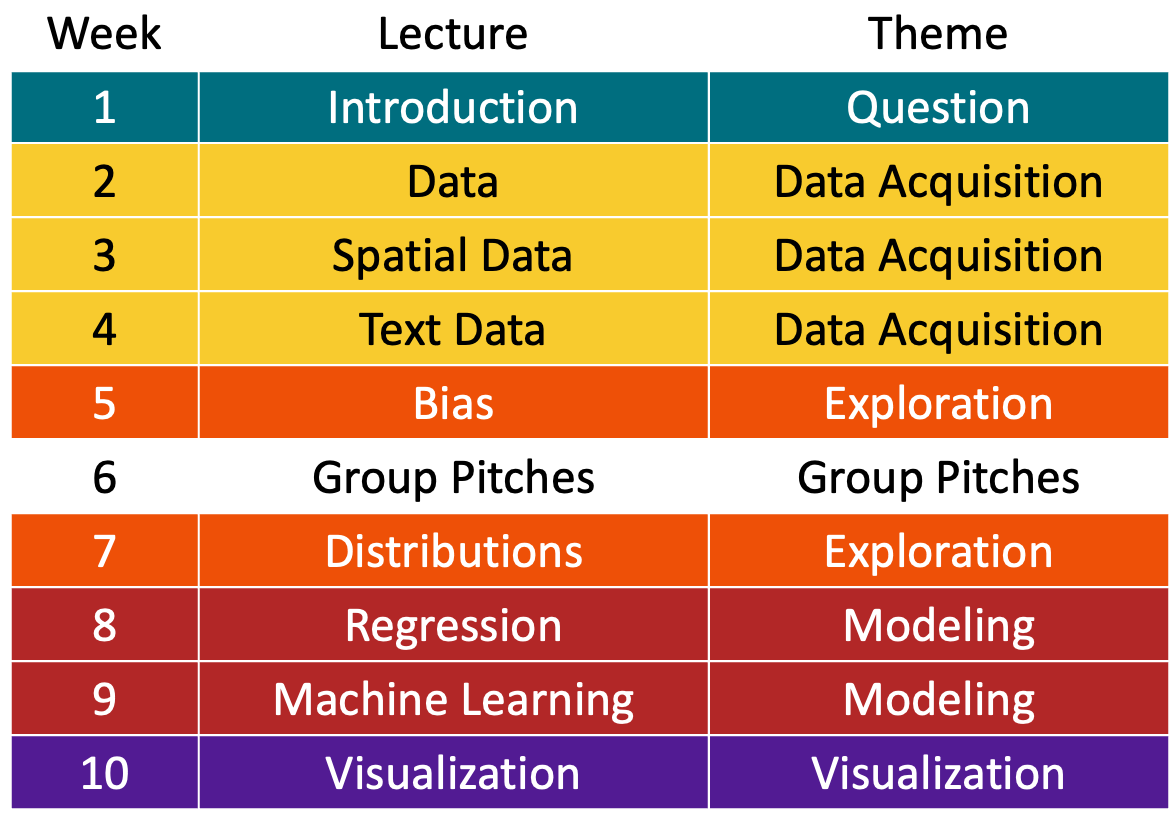
\includegraphics{./outline.png}

\bookmarksetup{startatroot}

\hypertarget{python-recap}{%
\chapter{Python Recap}\label{python-recap}}

\hypertarget{workshop-1-open-in-colab}{%
\section[\emph{Workshop 1} ]{\texorpdfstring{\emph{Workshop 1}
\href{https://colab.research.google.com/github/oballinger/QM2/blob/main/notebooks/W01.\%20Python\%20Recap.ipynb}{\protect
\includegraphics{notebooks/../colab-badge.png}}}{Workshop 1 Open In Colab}}\label{workshop-1-open-in-colab}}

\hypertarget{using-python}{%
\section{Using Python}\label{using-python}}

In this course, we'll make extensive use of \emph{Python}, a programming
language used widely in scientific computing and on the web. We will be
using Python as a way to manipulate, plot and analyse data. This isn't a
course about learning Python, it's about working with data - but we'll
learning a little bit of programming along the way.

By now, you should have done the prerequisites for the module, and
understand a bit about how Python is structured, what different commands
do, and so on - this is a bit of a refresher to remind you of what we
need at the beginning of term.

The particular flavour of Python we're using is \emph{iPython}, which,
as we've seen, allows us to combine text, code, images, equations and
figures in a \emph{Notebook}. This is a \emph{cell}, written in
\emph{markdown} - a way of writing nice text. Contrast this with
\emph{code} cell, which executes a bit of Python:

\begin{Shaded}
\begin{Highlighting}[]
\BuiltInTok{print}\NormalTok{(}\DecValTok{1}\OperatorTok{+}\DecValTok{1}\NormalTok{)}
\end{Highlighting}
\end{Shaded}

\begin{verbatim}
2
\end{verbatim}

The Notebook format allows you to engage in what Don Knuth describes as
\href{http://en.wikipedia.org/wiki/Literate_programming}{Literate
Programming}:

\begin{quote}
{[}\ldots{]} Instead of writing code containing documentation, the
literate programmer writes documentation containing code. No longer does
the English commentary injected into a program have to be hidden in
comment delimiters at the top of the file, or under procedure headings,
or at the end of lines. Instead, it is wrenched into the daylight and
made the main focus. The ``program'' then becomes primarily a document
directed at humans, with the code being herded between ``code
delimiters'' from where it can be extracted and shuffled out sideways to
the language system by literate programming tools.
\href{http://www.literateprogramming.com/lpquotes.html}{Ross Williams}
\end{quote}

\hypertarget{libraries}{%
\section{Libraries}\label{libraries}}

We will work with a number of \emph{libraries}, which provide additional
functions and techniques to help us to carry out our tasks.

These include:

\emph{Pandas:} we'll use this a lot to slice and dice data

\emph{matplotlib}: this is our basic graphing software, and we'll also
use it for mapping

\emph{nltk}: The Natural Language Tool Kit will help us work with text

We aren't doing all this to learn to program. We could spend a whole
term learning how to use Python and never look at any data, maps,
graphs, or visualisations. But we do need to understand a few basics to
use Python for working with data. So let's revisit a few concepts that
you should have covered in your prerequisites.

\hypertarget{variables}{%
\section{Variables}\label{variables}}

Python can broadly be divided in verbs and nouns: things which \emph{do}
things, and things which \emph{are} things. In Python, the verbs can be
\emph{commands}, \emph{functions}, or \emph{methods}. We won't worry too
much about the distinction here - suffice it to say, they are the parts
of code which manipulate data, calculate values, or show things on the
screen.

The simplest proper noun object in Python is the \emph{variable}.
Variables are given names and store information. This can be, for
example, numeric, text, or boolean (true/false). These are all
statements setting up variables:

n = 1

t = ``hi''

b = True

Now let's try this in code:

\begin{Shaded}
\begin{Highlighting}[]
\NormalTok{n }\OperatorTok{=} \DecValTok{1}

\NormalTok{t }\OperatorTok{=} \StringTok{"hi"}

\NormalTok{b }\OperatorTok{=} \VariableTok{True}
\end{Highlighting}
\end{Shaded}

Note that each command is on a new line; other than that, the
\emph{syntax} of Python should be fairly clear. We're setting these
variables equal to the letters and numbers and phrases and booleans.
\textbf{What's a boolean?}

The value of this is we now have values tied to these variables - so
every time we want to use it, we can refer to the variable:

\begin{Shaded}
\begin{Highlighting}[]
\NormalTok{n}
\end{Highlighting}
\end{Shaded}

\begin{verbatim}
1
\end{verbatim}

\begin{Shaded}
\begin{Highlighting}[]
\NormalTok{t}
\end{Highlighting}
\end{Shaded}

\begin{verbatim}
'hi'
\end{verbatim}

\begin{Shaded}
\begin{Highlighting}[]
\NormalTok{b}
\end{Highlighting}
\end{Shaded}

\begin{verbatim}
True
\end{verbatim}

Because we've defined these variables in the early part of the notebook,
we can use them later on.

\emph{\textbf{Advanced}: where do \textbf{classes} fit into this
noun/verb picture of variables and commands?}

\hypertarget{where-is-my-data}{%
\section{Where is my data?}\label{where-is-my-data}}

When we work in excel and text editors, we're used to seeing the data
onscreen - and if we manipulate the data in some way (averaging or
summing up), we see both the inputs and outputs on screen. The big
difference in working with Python is that we don't see our variables all
of the time, or the effect we're having on them. They're there in the
background, but it's usually worth checking in on them from time to
time, to see whether our processes are doing what we think they're
doing.

This is pretty easy to do - we can just type the variable name, or
``print(\emph{variable name})'':

\begin{Shaded}
\begin{Highlighting}[]
\NormalTok{n }\OperatorTok{=}\NormalTok{ n}\OperatorTok{+}\DecValTok{1}
\BuiltInTok{print}\NormalTok{(n)}
\BuiltInTok{print}\NormalTok{(t)}
\BuiltInTok{print}\NormalTok{(b)}
\end{Highlighting}
\end{Shaded}

\begin{verbatim}
2
hi
True
\end{verbatim}

\hypertarget{flow}{%
\section{Flow}\label{flow}}

Python, in common with all programming languages, executes commands in a
sequence - we might refer to this as the ``ineluctable march of the
machines'', but it's more common referred to as the \emph{flow} of the
code (we'll use the word ``code'' a lot - it just means commands written
in the programming language). In most cases, code just executes in the
order it's written. This is true within each \emph{cell} (each block of
text in the notebook), and it's true when we execute the cells in order;
that's why we can refer back to the variables we defined earlier:

\begin{Shaded}
\begin{Highlighting}[]
\BuiltInTok{print}\NormalTok{(n)}
\end{Highlighting}
\end{Shaded}

\begin{verbatim}
2
\end{verbatim}

If we make a change to one of these variables, say n:

\begin{Shaded}
\begin{Highlighting}[]
\NormalTok{n }\OperatorTok{=} \DecValTok{3}
\end{Highlighting}
\end{Shaded}

and execute the above ``print n'' command, you'll see that it has
changed n to 3. So if we go out of order, the obvious flow of the code
is confused. For this reason, try to write your code so it executes in
order, one cell at a time. At least for the moment, this will make it
easier to follow the logic of what you're doing to data.

\emph{Advanced}: what happens to this flow when you write
\emph{functions} to automate common tasks?

\textbf{\emph{Exercise - Setting up variables}}:

\begin{enumerate}
\def\labelenumi{\arabic{enumi}.}
\item
  Create a new cell.
\item
  Create the variables ``name'', and assign your name to it.
\item
  Create a variable ``Python'' and assign a score out of 10 to how much
  you like Python.
\item
  Create a variable ``prior'' and if you've used Python before, assign
  True; otherwise assign False to the variable
\item
  Print these out to the screen
\end{enumerate}

\hypertarget{downloading-data}{%
\section{Downloading Data}\label{downloading-data}}

Lets fetch the data we will be using for this session. There are two
ways in which you can upload data to the Colab notebook. You can use the
following code to upload a CSV or similar data file.

\begin{Shaded}
\begin{Highlighting}[]
\ImportTok{from}\NormalTok{ google.colab }\ImportTok{import}\NormalTok{ files}
\NormalTok{uploaded }\OperatorTok{=}\NormalTok{ files.upload()}
\end{Highlighting}
\end{Shaded}

\begin{verbatim}
ModuleNotFoundError: No module named 'google.colab'
\end{verbatim}

Or you can use the following cell to fetch the data directly from the
QM2 server.

Let's create a folder that we can store all our data for this session

\begin{Shaded}
\begin{Highlighting}[]
\OperatorTok{!}\NormalTok{mkdir data}
\end{Highlighting}
\end{Shaded}

\begin{Shaded}
\begin{Highlighting}[]
\OperatorTok{!}\NormalTok{mkdir .}\OperatorTok{/}\NormalTok{data}\OperatorTok{/}\NormalTok{wk1}
\OperatorTok{!}\NormalTok{curl https:}\OperatorTok{//}\NormalTok{s3.eu}\OperatorTok{{-}}\NormalTok{west}\OperatorTok{{-}}\FloatTok{2.}\ErrorTok{amazonaws}\NormalTok{.com}\OperatorTok{/}\NormalTok{qm2}\OperatorTok{/}\NormalTok{wk1}\OperatorTok{/}\NormalTok{data.csv }\OperatorTok{{-}}\NormalTok{o .}\OperatorTok{/}\NormalTok{data}\OperatorTok{/}\NormalTok{wk1}\OperatorTok{/}\NormalTok{data.csv}
\OperatorTok{!}\NormalTok{curl https:}\OperatorTok{//}\NormalTok{s3.eu}\OperatorTok{{-}}\NormalTok{west}\OperatorTok{{-}}\FloatTok{2.}\ErrorTok{amazonaws}\NormalTok{.com}\OperatorTok{/}\NormalTok{qm2}\OperatorTok{/}\NormalTok{wk1}\OperatorTok{/}\NormalTok{sample\_group.csv }\OperatorTok{{-}}\NormalTok{o .}\OperatorTok{/}\NormalTok{data}\OperatorTok{/}\NormalTok{wk1}\OperatorTok{/}\NormalTok{sample\_group.csv}
\end{Highlighting}
\end{Shaded}

\begin{verbatim}
  % Total    % Received % Xferd  Average Speed   Time    Time     Time  Current
                                 Dload  Upload   Total   Spent    Left  Speed
100   203  100   203    0     0    527      0 --:--:-- --:--:-- --:--:--   527
  % Total    % Received % Xferd  Average Speed   Time    Time     Time  Current
                                 Dload  Upload   Total   Spent    Left  Speed
100   297  100   297    0     0    838      0 --:--:-- --:--:-- --:--:--   836
\end{verbatim}

\hypertarget{storing-and-importing-data}{%
\section{Storing and importing data}\label{storing-and-importing-data}}

Typically, data we look at won't be just one number, or one bit of text.
Python has a lot of different ways of dealing with a bunch of numbers:
for example, a list of values is called a \textbf{list}:

\begin{Shaded}
\begin{Highlighting}[]
\NormalTok{listy }\OperatorTok{=}\NormalTok{ [}\DecValTok{1}\NormalTok{,}\DecValTok{2}\NormalTok{,}\DecValTok{3}\NormalTok{,}\DecValTok{6}\NormalTok{,}\DecValTok{9}\NormalTok{]}
\BuiltInTok{print}\NormalTok{(listy)}
\end{Highlighting}
\end{Shaded}

\begin{verbatim}
[1, 2, 3, 6, 9]
\end{verbatim}

A set of values \emph{linked} to an index (or key) is called a
\textbf{dictionary}; for example:

\begin{Shaded}
\begin{Highlighting}[]
\NormalTok{dicty }\OperatorTok{=}\NormalTok{ \{}\StringTok{\textquotesingle{}Bob\textquotesingle{}}\NormalTok{: }\FloatTok{1.2}\NormalTok{, }\StringTok{\textquotesingle{}Mike\textquotesingle{}}\NormalTok{: }\FloatTok{1.2}\NormalTok{, }\StringTok{\textquotesingle{}Coop\textquotesingle{}}\NormalTok{: }\FloatTok{1.1}\NormalTok{, }\StringTok{\textquotesingle{}Maddy\textquotesingle{}}\NormalTok{: }\FloatTok{1.3}\NormalTok{, }\StringTok{\textquotesingle{}Giant\textquotesingle{}}\NormalTok{: }\FloatTok{2.1}\NormalTok{\}}
\BuiltInTok{print}\NormalTok{(dicty)}
\end{Highlighting}
\end{Shaded}

\begin{verbatim}
{'Bob': 1.2, 'Mike': 1.2, 'Coop': 1.1, 'Maddy': 1.3, 'Giant': 2.1}
\end{verbatim}

Notice that the list uses square brackets with values separated by
commas, and the dict uses curly brackets with pairs separated by commas,
and colons (:) to link a \emph{key} (index or address) with a value.

(You might notice that they haven't printed out in the order you entered
them)

*\textbf{Advanced}: Print out 1) The third element of \textbf{listy},
and 2) The element of \textbf{dicty} relating to Giant

We'll discuss different ways of organising data again soon, but for now
we'll look at \emph{dataframes} - the way our data-friendly
\emph{library} \textbf{Pandas} works with data. We'll be using Pandas a
lot this term, so it's good to get started with it early.

Let's start by importing pandas. We'll also import another library, but
we're not going to worry about that too much at the moment.

If you see a warning about `Building Font Cache' don't worry - this is
normal.

\begin{Shaded}
\begin{Highlighting}[]
\ImportTok{import}\NormalTok{ pandas}

\ImportTok{import}\NormalTok{ matplotlib}
\OperatorTok{\%}\NormalTok{matplotlib inline}
\end{Highlighting}
\end{Shaded}

Let's import a simple dataset and show it in pandas. We'll use a
pre-prepared ``.csv'' file, which needs to be in the same folder as our
code.

\begin{Shaded}
\begin{Highlighting}[]
\NormalTok{data }\OperatorTok{=}\NormalTok{ pandas.read\_csv(}\StringTok{\textquotesingle{}./data/wk1/data.csv\textquotesingle{}}\NormalTok{)}
\NormalTok{data.head()}
\end{Highlighting}
\end{Shaded}

\begin{longtable}[]{@{}llllll@{}}
\toprule()
& Name & First Appearance & Approx height & Gender & Law Enforcement \\
\midrule()
\endhead
0 & Bob & 1.2 & 6.0 & Male & False \\
1 & Mike & 1.2 & 5.5 & Male & False \\
2 & Coop & 1.1 & 6.0 & Male & True \\
3 & Maddy & 1.3 & 5.5 & Female & False \\
4 & Giant & 2.1 & 7.5 & Male & False \\
\bottomrule()
\end{longtable}

What we've done here is read in a .csv file into a dataframe, the object
pandas uses to work with data, and one that has lots of methods for
slicing and dicing data, as we will see over the coming weeks. The
head() command tells iPython to show the first few columns/rows of the
data, so we can start to get a sense of what the data looks like and
what sort of type of objects is represents.

\bookmarksetup{startatroot}

\hypertarget{supplementary-kaggle-exercises}{%
\chapter{Supplementary: Kaggle
exercises}\label{supplementary-kaggle-exercises}}

If you've gotten this far, congratulations! To further hone your skills,
try working your way through the five
\href{https://www.kaggle.com/learn/intro-to-programming}{intro to
programming notebooks on Kaggle}. These cover a range of skills that
we'll be using throughout the term. Kaggle is a very useful resource for
learning data science, so making an account may not be a bad idea!

\bookmarksetup{startatroot}

\hypertarget{intro-to-pandas}{%
\chapter{Intro to Pandas}\label{intro-to-pandas}}

\hypertarget{workshop-2-open-in-colab}{%
\section[\emph{Workshop 2} ]{\texorpdfstring{\emph{Workshop 2}
\href{https://colab.research.google.com/github/oballinger/QM2/blob/main/notebooks/W02.\%20Pandas.ipynb}{\protect
\includegraphics{notebooks/../colab-badge.png}}}{Workshop 2 Open In Colab}}\label{workshop-2-open-in-colab}}

In this workshop, our aim is to get used to working with more complex
data that we've imported from external files. We'll start to graph it,
and to slice and dice it, to select the bits we're interested in.

We will work with \emph{pandas} to manipulate the data, and to derive
measures and graphs that tell us a bit more than what the source data
files tell us.

\hypertarget{aims}{%
\subsection{Aims}\label{aims}}

\begin{itemize}
\tightlist
\item
  Learn to import data to python using pandas
\item
  Learn how access specific rows, columns and cells
\item
  Plot the data
\item
  Tidy up graphs to include axes
\end{itemize}

\hypertarget{introduction}{%
\section{Introduction}\label{introduction}}

We are going to work with some UK income data. The income data is
packaged as a .csv file. The Pandas package knows how to handle this and
put the data in a DataFrame, as we've seen. Let's examine the data and
start to see what we can say about it. First of all, we have to find
data - I'm interested in looking in data with a wide spread, so I looked
for data on income in the UK.

This data is collected by the Office for National Statistics(ONS) :
http://www.ons.gov.uk/ons/datasets-and-tables/index.html?pageSize=50\&sortBy=none\&sortDirection=none\&newquery=income+percentile
- but the exact data I want to see, income by percentile, is tricky to
find.

I ended up using data from 2011, generated from a study called the
Family Resources Survey and collated and tweaked by an independent
research unit called the Institute of Fiscal Studies (IFS). The
``tweaking'' they do tends to be around the size of the family unit, and
other factors which create economies of scale - hence they
``equivalise'' it. The IFS is quoted in UK Government documents, so we
can have some trust in their impartiality, or at least accuracy - of
course, if we were publishing research about this, that's not really
good enough and we'd want to reproduce, or at least understand and
critique, their methodology rather than just trusting it!

e.g.:

http://www.ifs.org.uk/wheredoyoufitin/about.php

https://en.wikipedia.org/wiki/Equivalisation

\hypertarget{downloading-the-data}{%
\section{Downloading the Data}\label{downloading-the-data}}

Let's grab our income data from our course website and save it into our
data folder. If you've not already created a data folder then do so
using the following command. Don't worry if it generates an error, that
means you've already got a data folder.

\begin{Shaded}
\begin{Highlighting}[]
\OperatorTok{!}\NormalTok{mkdir data}
\end{Highlighting}
\end{Shaded}

\begin{verbatim}
mkdir: data: File exists
\end{verbatim}

\begin{Shaded}
\begin{Highlighting}[]
\OperatorTok{!}\NormalTok{mkdir data}\OperatorTok{/}\NormalTok{wk2}
\OperatorTok{!}\NormalTok{curl https:}\OperatorTok{//}\NormalTok{github.com}\OperatorTok{/}\NormalTok{oballinger}\OperatorTok{/}\NormalTok{QM2}\OperatorTok{/}\NormalTok{blob}\OperatorTok{/}\NormalTok{main}\OperatorTok{/}\NormalTok{notebooks}\OperatorTok{/}\NormalTok{data}\OperatorTok{/}\NormalTok{wk2}\OperatorTok{/}\NormalTok{incomes.csv }\OperatorTok{{-}}\NormalTok{o .}\OperatorTok{/}\NormalTok{data}\OperatorTok{/}\NormalTok{wk2}\OperatorTok{/}\NormalTok{incomes.csv}
\end{Highlighting}
\end{Shaded}

\begin{verbatim}
mkdir: data/wk2: File exists
  % Total    % Received % Xferd  Average Speed   Time    Time     Time  Current
                                 Dload  Upload   Total   Spent    Left  Speed
100 15154  100 15154    0     0   135k      0 --:--:-- --:--:-- --:--:--  143k
\end{verbatim}

\begin{Shaded}
\begin{Highlighting}[]
\ImportTok{import}\NormalTok{ pandas}
\ImportTok{import}\NormalTok{ pylab}
\ImportTok{import}\NormalTok{ matplotlib.pyplot }\ImportTok{as}\NormalTok{ plt}
\CommentTok{\# make the plots a little wider by default}
\OperatorTok{\%}\NormalTok{matplotlib inline}
\NormalTok{plt.style.use(}\StringTok{\textquotesingle{}ggplot\textquotesingle{}}\NormalTok{)}

\NormalTok{pylab.rcParams[}\StringTok{\textquotesingle{}figure.figsize\textquotesingle{}}\NormalTok{] }\OperatorTok{=}\NormalTok{ (}\FloatTok{10.}\NormalTok{, }\FloatTok{8.}\NormalTok{)}
\end{Highlighting}
\end{Shaded}

\begin{Shaded}
\begin{Highlighting}[]
\NormalTok{data\_path }\OperatorTok{=} \StringTok{"./data/wk2/incomes.csv"}

\NormalTok{income }\OperatorTok{=}\NormalTok{  pandas.read\_csv(data\_path, index\_col}\OperatorTok{=}\DecValTok{0}\NormalTok{)}
\NormalTok{income.head()}
\end{Highlighting}
\end{Shaded}

\begin{longtable}[]{@{}llllllllllllllll@{}}
\toprule()
& Net equivalised household income in 2010-11, week & Childless couple,
annual income & Couple, two children under 14 & Couple, three children
under 14 & Couple with one child under 14 & Couple with two children
aged 15 to 18 & Couple, two children under 14 plus dependent adult &
Single adult & Lone parent, one child under 14 & Lone parent, two
children under 14 & Lone parent, two children aged 15-18 & ANNOTATIONS &
1979 to 1996-97 & 1996-97 to 2009-10 & 1996-97 to 2010-11 \\
Percentile Point & & & & & & & & & & & & & & & \\
\midrule()
\endhead
1 & 33.50 & 1,746.92 & 2,445.69 & 2,795.08 & 2,096.31 & 2,899.89 &
3,022.18 & 1,170.44 & 1,519.82 & 1,869.21 & 2,323.41 & NaN & NaN & NaN &
NaN \\
2 & 98.60 & 5,141.01 & 7,197.41 & 8,225.61 & 6,169.21 & 8,534.07 &
8,893.95 & 3,444.48 & 4,472.68 & 5,500.88 & 6,837.54 & NaN & -0.20\% &
-1.30\% & -0.50\% \\
3 & 128.56 & 6,703.11 & 9,384.36 & 10,724.98 & 8,043.74 & 11,127.17 &
11,596.39 & 4,491.09 & 5,831.71 & 7,172.33 & 8,915.14 & NaN & 0.40\% &
0.10\% & 0.10\% \\
4 & 151.05 & 7,875.75 & 11,026.05 & 12,601.20 & 9,450.90 & 13,073.75 &
13,625.05 & 5,276.75 & 6,851.90 & 8,427.05 & 10,474.75 & NaN & 0.50\% &
0.80\% & 0.60\% \\
5 & 166.32 & 8,671.91 & 12,140.68 & 13,875.06 & 10,406.30 & 14,395.38 &
15,002.41 & 5,810.18 & 7,544.57 & 9,278.95 & 11,533.65 & NaN & 0.70\% &
1.00\% & 0.90\% \\
\bottomrule()
\end{longtable}

This is a simple dataframe - we see the percentile and an income. Note
that I've told pandas to use the first column (the Percentile) as the
index to make life easier.

The percentile tells us how people on that income rank - so the final
category, 99\% (which is really binned, so 99\%\textless n\(\leq\)
100\%), is telling us how much ``the 1\%'' earn. Let's find out:

\begin{Shaded}
\begin{Highlighting}[]
\NormalTok{income.tail()}
\end{Highlighting}
\end{Shaded}

\begin{longtable}[]{@{}llllllllllllllll@{}}
\toprule()
& Net equivalised household income in 2010-11, week & Childless couple,
annual income & Couple, two children under 14 & Couple, three children
under 14 & Couple with one child under 14 & Couple with two children
aged 15 to 18 & Couple, two children under 14 plus dependent adult &
Single adult & Lone parent, one child under 14 & Lone parent, two
children under 14 & Lone parent, two children aged 15-18 & ANNOTATIONS &
1979 to 1996-97 & 1996-97 to 2009-10 & 1996-97 to 2010-11 \\
Percentile Point & & & & & & & & & & & & & & & \\
\midrule()
\endhead
95 & 1075.73 & 56,088.56 & 78,523.99 & 89,741.70 & 67,306.27 & 93,107.01
& 97,033.21 & 37,579.34 & 48,797.05 & 60,014.76 & 74,597.79 & NaN &
2.90\% & 2.00\% & 1.30\% \\
96 & 1174.48 & 61,237.18 & 85,732.05 & 97,979.49 & 73,484.61 &
101,653.72 & 105,940.32 & 41,028.91 & 53,276.35 & 65,523.78 & 81,445.45
& NaN & 3.00\% & 2.00\% & 1.40\% \\
97 & 1302.74 & 67,925.07 & 95,095.10 & 108,680.12 & 81,510.09 &
112,755.62 & 117,510.37 & 45,509.80 & 59,094.81 & 72,679.83 & 90,340.35
& NaN & 3.20\% & 2.20\% & 1.60\% \\
98 & 1523.31 & 79,425.23 & 111,195.32 & 127,080.36 & 95,310.27 &
131,845.88 & 137,405.64 & 53,214.90 & 69,099.95 & 84,984.99 & 105,635.55
& NaN & 3.20\% & 2.70\% & 1.70\% \\
99 & 2090.35 & 108,990.74 & 152,587.04 & 174,385.19 & 130,788.89 &
180,924.64 & 188,553.99 & 73,023.80 & 94,821.95 & 116,620.10 &
144,957.69 & NaN & NaN & NaN & NaN \\
\bottomrule()
\end{longtable}

Well, they we have it - the 1\% earn, on average, about £2000 a week.
How does that compare to people in the 90\% decile? We can access
particular \emph{rows} in a dataframe using \textbf{.loc{[}row
index{]}}; because our index is the percentile point, we can just read
it off:

\begin{Shaded}
\begin{Highlighting}[]
\NormalTok{income.loc[}\DecValTok{90}\NormalTok{]}
\end{Highlighting}
\end{Shaded}

\begin{verbatim}
Net equivalised household income in 2010-11, week        845.54
Childless couple, annual income                       44,086.54
Couple, two children under 14                         61,721.15
Couple, three children under 14                       70,538.46
Couple with one child under 14                        52,903.85
Couple with two children aged 15 to 18                73,183.65
Couple, two children under 14 plus dependent adult    76,269.71
Single adult                                          29,537.98
Lone parent, one child under 14                       38,355.29
Lone parent, two children under 14                    47,172.60
Lone parent, two children aged 15-18                  58,635.10
ANNOTATIONS                                                 NaN
1979 to 1996-97                                           2.50%
1996-97 to 2009-10                                        1.70%
1996-97 to 2010-11                                        1.20%
Name: 90, dtype: object
\end{verbatim}

We can also select a range of values with the ``colon'' notation. This
will select the 90-95th percentiles, for example:

\begin{Shaded}
\begin{Highlighting}[]
\NormalTok{income.loc[}\DecValTok{90}\NormalTok{:}\DecValTok{95}\NormalTok{]}
\end{Highlighting}
\end{Shaded}

\begin{longtable}[]{@{}llllllllllllllll@{}}
\toprule()
& Net equivalised household income in 2010-11, week & Childless couple,
annual income & Couple, two children under 14 & Couple, three children
under 14 & Couple with one child under 14 & Couple with two children
aged 15 to 18 & Couple, two children under 14 plus dependent adult &
Single adult & Lone parent, one child under 14 & Lone parent, two
children under 14 & Lone parent, two children aged 15-18 & ANNOTATIONS &
1979 to 1996-97 & 1996-97 to 2009-10 & 1996-97 to 2010-11 \\
Percentile Point & & & & & & & & & & & & & & & \\
\midrule()
\endhead
90 & 845.54 & 44,086.54 & 61,721.15 & 70,538.46 & 52,903.85 & 73,183.65
& 76,269.71 & 29,537.98 & 38,355.29 & 47,172.60 & 58,635.10 & NaN &
2.50\% & 1.70\% & 1.20\% \\
91 & 876.63 & 45,707.74 & 63,990.84 & 73,132.39 & 54,849.29 & 75,874.85
& 79,074.40 & 30,624.19 & 39,765.74 & 48,907.29 & 60,791.30 & NaN &
2.60\% & 1.70\% & 1.20\% \\
92 & 911.29 & 47,514.54 & 66,520.35 & 76,023.26 & 57,017.44 & 78,874.13
& 82,200.15 & 31,834.74 & 41,337.65 & 50,840.55 & 63,194.33 & NaN &
2.60\% & 1.80\% & 1.20\% \\
93 & 957.14 & 49,905.23 & 69,867.32 & 79,848.36 & 59,886.27 & 82,842.68
& 86,336.04 & 33,436.50 & 43,417.55 & 53,398.59 & 66,373.95 & NaN &
2.70\% & 1.80\% & 1.30\% \\
94 & 1016.37 & 52,993.38 & 74,190.73 & 84,789.40 & 63,592.05 & 87,969.00
& 91,678.54 & 35,505.56 & 46,104.24 & 56,702.91 & 70,481.19 & NaN &
2.90\% & 1.90\% & 1.30\% \\
95 & 1075.73 & 56,088.56 & 78,523.99 & 89,741.70 & 67,306.27 & 93,107.01
& 97,033.21 & 37,579.34 & 48,797.05 & 60,014.76 & 74,597.79 & NaN &
2.90\% & 2.00\% & 1.30\% \\
\bottomrule()
\end{longtable}

\hypertarget{accessing-parts-of-a-dataframe}{%
\section{Accessing parts of a
dataframe}\label{accessing-parts-of-a-dataframe}}

If we want to extract the actual value instead of just the whole row, we
need to reference the \emph{column} as well as the row. In pandas,
columns are referenced by \textbf{column name}:

\begin{Shaded}
\begin{Highlighting}[]
\NormalTok{income[}\StringTok{\textquotesingle{}Net equivalised household income in 2010{-}11, week\textquotesingle{}}\NormalTok{]}
\end{Highlighting}
\end{Shaded}

\begin{verbatim}
Percentile Point
1       33.50
2       98.60
3      128.56
4      151.05
5      166.32
       ...   
95    1075.73
96    1174.48
97    1302.74
98    1523.31
99    2090.35
Name: Net equivalised household income in 2010-11, week, Length: 99, dtype: float64
\end{verbatim}

So, to access a particular cell, we tell Python the row and the column
(this is pretty simple - the same way we tell excel to access cell
``A34'' meaning Column A, Row 34). One way we do that in pandas is to
select the column, and then use .loc{[}{]} on the index.

\begin{Shaded}
\begin{Highlighting}[]
\NormalTok{income[}\StringTok{\textquotesingle{}Net equivalised household income in 2010{-}11, week\textquotesingle{}}\NormalTok{].loc[}\DecValTok{90}\NormalTok{]}
\end{Highlighting}
\end{Shaded}

\begin{verbatim}
845.54
\end{verbatim}

We've accessed row 90 of the column called `Net equivalised household
income in 2010-11, week'; can we access the data the other way around -
can we first take the row and then specify a column? Let's try:

\begin{Shaded}
\begin{Highlighting}[]
\NormalTok{income.loc[}\DecValTok{90}\NormalTok{][}\StringTok{\textquotesingle{}Net equivalised household income in 2010{-}11, week\textquotesingle{}}\NormalTok{]}
\end{Highlighting}
\end{Shaded}

\begin{verbatim}
845.54
\end{verbatim}

Yes, this seems to be working fine.

\hypertarget{extension}{%
\subsection{Extension}\label{extension}}

The reason for this is that selecting the column spits out a smaller
dataframe, and all dataframes use ``loc'', so we can use that. Another
way to do this would be to use an explicit variable for the dataframe,
along the lines of:

\texttt{smallDataFrame\ =\ income{[}\textquotesingle{}Net\ equivalised\ household\ income\ in\ 2010-11,\ week\textquotesingle{}{]}}\strut \\
\texttt{smallDataFrame.loc{[}90{]}}

by doing income

\texttt{{[}\textquotesingle{}Net\ equivalised\ household\ income\ in\ 2010-11,\ week\textquotesingle{}{]}.loc{[}90{]}}

we're taking the ``smallDataFrame'' object as an implicit (or hidden)
output

If we want to look at a few rows of data, we can use a range:

\begin{Shaded}
\begin{Highlighting}[]
\NormalTok{income[}\StringTok{\textquotesingle{}Net equivalised household income in 2010{-}11, week\textquotesingle{}}\NormalTok{].loc[}\DecValTok{90}\NormalTok{:}\DecValTok{95}\NormalTok{]}
\end{Highlighting}
\end{Shaded}

\begin{verbatim}
Percentile Point
90     845.54
91     876.63
92     911.29
93     957.14
94    1016.37
95    1075.73
Name: Net equivalised household income in 2010-11, week, dtype: float64
\end{verbatim}

So, to recap, we can now access a particular \textbf{row} using
\emph{loc{[}index number{]}}, a particular \textbf{column} with the
square brackets formalism \emph{dataframename{[}`column name'{]}}, or
both \emph{dataframename{[}`column name'{]}.loc{[}index number{]}}.
We've made a start at being able to get to the bits of data we need.

\hypertarget{exercise}{%
\section{Exercise:}\label{exercise}}

How do the equivalised incomes of single adults and childless couples
compare? Look at the 1st, 99th and 50th percentile and summarise what
this tells you about the value or price of coupling.

\hypertarget{examining-the-distribution}{%
\section{Examining the Distribution}\label{examining-the-distribution}}

Returning to the overall statistics, the 90\% percentile earns less than
half the top percentile (``the 1\%''); if you're taking home over £800
as a household, you're in the top 10\% of earners.

How does 1. The income of ``the 1\%'' compare with the mean and median
across the population, as a proportion? 2. How does the 1\% compare with
the 90th percentile (the 10\%)? 3. How does the 10\% compare with the
median and mean?

The 1\% earn about 60 times the poorest groups in society - and we've
made other comparisons. But that's not the whole story. Let's look at
the income graph.

In pandas, we can plot this fairly easily\ldots{}

\begin{Shaded}
\begin{Highlighting}[]
\NormalTok{income[}\StringTok{\textquotesingle{}Net equivalised household income in 2010{-}11, week\textquotesingle{}}\NormalTok{].plot()}
\NormalTok{plt.title(}\StringTok{\textquotesingle{}UK Net Equivalised Income by Percentile per week, 2010{-}11\textquotesingle{}}\NormalTok{)}
\NormalTok{plt.xlabel(}\StringTok{\textquotesingle{}Income Percentile\textquotesingle{}}\NormalTok{)}
\NormalTok{plt.ylabel(}\StringTok{\textquotesingle{}Income (Net, Equivalised) [GBP]\textquotesingle{}}\NormalTok{)}
\end{Highlighting}
\end{Shaded}

\begin{verbatim}
Text(0, 0.5, 'Income (Net, Equivalised) [GBP]')
\end{verbatim}

\begin{figure}[H]

{\centering \includegraphics{notebooks/W02. Pandas_files/figure-pdf/cell-13-output-2.png}

}

\end{figure}

We see a curve that is pretty linear in the middle region, but curves
rapidly upwards in the higher percentile and looks more like a power
law.

\hypertarget{exercise-means}{%
\subsection{Exercise: Means}\label{exercise-means}}

Where does the mean appear here? Draw in a horizontal line to show the
mean using \textbf{axhline}. Show the median on the same graph. What is
the meaning of the median in this context?

Hint: Recall that last time we used \emph{axvline} to highlight the mean
and standard deviation by drawing vertical lines on the axis. Here, we
use \emph{axhline} to draw horizontal lines.

\hypertarget{extension-accessing-cells}{%
\subsection{Extension: Accessing
cells}\label{extension-accessing-cells}}

There are a number of ways to access elements of the dataframe: we've
shown how to access columns by the {[}\emph{`name of column'}{]} method,
and rows via the .loc{[}\emph{index}{]} method; and how we can select a
range. There are also .iloc methods to select by number rather than
name; you should become familiar with these on the documentation page
for pandas.

\hypertarget{comparing-segments}{%
\section{Comparing segments}\label{comparing-segments}}

Earlier, we compared some summary statistics of single people and
couples. Let's look at the wider curve for more than one group, now:

\begin{Shaded}
\begin{Highlighting}[]
\CommentTok{\#This is going to throw a load of errors}
\NormalTok{income[[}\StringTok{\textquotesingle{}Single adult\textquotesingle{}}\NormalTok{,}\StringTok{\textquotesingle{}Lone parent, one child under 14\textquotesingle{}}\NormalTok{]].plot()}
\end{Highlighting}
\end{Shaded}

\begin{verbatim}
TypeError: no numeric data to plot
\end{verbatim}

\hypertarget{warning}{%
\section{Warning}\label{warning}}

This isn't looking good. There's a load of text and no graph. If you've
not seen this before, it's an error - something has gone wrong.
Generally, if we look at the \textbf{final} line, it should tell us
what's wrong, in this case there's ``no numeric data to plot'', which is
weird, because we've seen the data and have even plotted some of it.

\hypertarget{messy-data}{%
\section{Messy Data}\label{messy-data}}

DataFrames, as we are starting to see, give us the chance to plot, chop,
slice and data to help us make sense of it. Here, we will create a
\textbf{new} DataFrame to take only two columns of data, and get rid of
any blank cells and any cells which are not being read as numbers -
normally a sign of a missing value or a non-numerical character. Why
could this be happening? It could be

\begin{itemize}
\item
  due to blank spaces in the text file
\item
  due to letters where there should be numbers
\item
  due to characters (``,'', ``-'', etc) that shouldn't really be there
\end{itemize}

In general, there will be some detective work required to figure out
what's wrong in our text file. Your best bet is sometimes to open up the
data in a text editor, like I've done here:

\begin{Shaded}
\begin{Highlighting}[]
\ImportTok{from}\NormalTok{ IPython.display }\ImportTok{import}\NormalTok{ Image}

\NormalTok{data\_path }\OperatorTok{=} \StringTok{"https://s3.eu{-}west{-}2.amazonaws.com/qm2/wk2/data.png"}
\NormalTok{Image(data\_path)}
\end{Highlighting}
\end{Shaded}

\begin{figure}[H]

{\centering 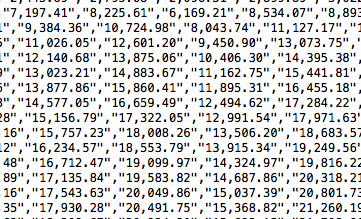
\includegraphics{notebooks/W02. Pandas_files/figure-pdf/cell-15-output-1.png}

}

\end{figure}

That's a screenshot of our datafile, opened up in a text editor. As we
can see, these numbers are separated by commas and surrounded by
quotation marks - this is normal, and what .csv files are supposed to
look like. However, there are a lot of commas within the numbers - which
makes it easier for people to read, but confuses software. Luckily,
Python has a method for dealing with this - the ``replace'' method.

Unfortunately, this dataframe is quite messy, so I'm going to have to
extract just the columns of data I'm interested in to make it work. I'll
do that by creating a new dataframe:

\hypertarget{example-cleaning-data}{%
\section{Example: Cleaning data}\label{example-cleaning-data}}

\begin{Shaded}
\begin{Highlighting}[]
\NormalTok{clean }\OperatorTok{=}\NormalTok{ income[[}\StringTok{\textquotesingle{}Childless couple, annual income\textquotesingle{}}\NormalTok{,}\StringTok{\textquotesingle{}Couple, two children under 14\textquotesingle{}}\NormalTok{]]}
\NormalTok{clean.head()}
\end{Highlighting}
\end{Shaded}

\begin{longtable}[]{@{}lll@{}}
\toprule()
& Childless couple, annual income & Couple, two children under 14 \\
Percentile Point & & \\
\midrule()
\endhead
1 & 1,746.92 & 2,445.69 \\
2 & 5,141.01 & 7,197.41 \\
3 & 6,703.11 & 9,384.36 \\
4 & 7,875.75 & 11,026.05 \\
5 & 8,671.91 & 12,140.68 \\
\bottomrule()
\end{longtable}

We see those pesky commas. Now we can get on with cleaning up the data:

\begin{Shaded}
\begin{Highlighting}[]
\NormalTok{clean}\OperatorTok{=}\NormalTok{clean.replace(}\StringTok{\textquotesingle{},\textquotesingle{}}\NormalTok{, }\StringTok{\textquotesingle{}\textquotesingle{}}\NormalTok{, regex}\OperatorTok{=}\VariableTok{True}\NormalTok{)}

\CommentTok{\# In addition, missing values are sometimes written as \textquotesingle{}{-}\textquotesingle{}, in order for Python to understand that it is just a missing numerical }
\CommentTok{\# value, all \textquotesingle{}{-}\textquotesingle{} need to be replaced with \textquotesingle{}NaN\textquotesingle{}.}
\NormalTok{clean }\OperatorTok{=}\NormalTok{ clean.replace(}\StringTok{\textquotesingle{}{-}\textquotesingle{}}\NormalTok{, }\StringTok{\textquotesingle{}NaN\textquotesingle{}}\NormalTok{, regex}\OperatorTok{=}\VariableTok{True}\NormalTok{).astype(}\StringTok{\textquotesingle{}float\textquotesingle{}}\NormalTok{)}
\NormalTok{clean.head()}
\end{Highlighting}
\end{Shaded}

\begin{longtable}[]{@{}lll@{}}
\toprule()
& Childless couple, annual income & Couple, two children under 14 \\
Percentile Point & & \\
\midrule()
\endhead
1 & 1746.92 & 2445.69 \\
2 & 5141.01 & 7197.41 \\
3 & 6703.11 & 9384.36 \\
4 & 7875.75 & 11026.05 \\
5 & 8671.91 & 12140.68 \\
\bottomrule()
\end{longtable}

\textbf{Extension}: ``\textbf{Regex}'' refers to ``\textbf{Reg}ular
\textbf{Ex}pression'', which is a way of replacing and cleaning text.
It's a bit beyond the scope of this class, but worth looking into if
you're interested in programming more widely.

This seems to have done the job. We've also put a line in the code to
get rid of dashes - a way that data collectors will sometimes represent
missing data. Now let's plot this.

\hypertarget{asking-more-questions-of-the-data}{%
\section{Asking more questions of the
data}\label{asking-more-questions-of-the-data}}

For me, this data starts to beg further questions. How would we answer
these?

\begin{itemize}
\item
  If the top 20\% of income shows such a sharp increase, how do we know
  that there isn't a similar uptick \emph{within} the 1\%? We've already
  seen that the mean of the dataset as a whole is much less than the
  half the maximum category (it's 25\% of the maximum). What if that's
  true within the 1\%, and £2,000/week as a fraction of the 0.1\%, or
  the 0.01\%?
\item
  How does this break down for gender, or educational background, or
  other factors like ethnicity or country of origin?
\item
  Which parts of the income curve show greater gaps between these
  subgroups and what might it say about the underlying causal
  mechanisms?
\end{itemize}

\begin{Shaded}
\begin{Highlighting}[]
\NormalTok{clean.plot()}
\NormalTok{plt.title(}\StringTok{\textquotesingle{}A Modest Proposal: The fiscal benefits of childbirth\textquotesingle{}}\NormalTok{)}
\NormalTok{plt.xlabel(}\StringTok{\textquotesingle{}Percentile\textquotesingle{}}\NormalTok{)}
\NormalTok{plt.ylabel(}\StringTok{\textquotesingle{}Income Per Week [GBP]\textquotesingle{}}\NormalTok{)}
\end{Highlighting}
\end{Shaded}

\begin{verbatim}
Text(0, 0.5, 'Income Per Week [GBP]')
\end{verbatim}

\begin{figure}[H]

{\centering \includegraphics{notebooks/W02. Pandas_files/figure-pdf/cell-18-output-2.png}

}

\end{figure}

\hypertarget{exercise-1}{%
\section{Exercise:}\label{exercise-1}}

Previously, we'd examined income gaps between single people and couples
(how very romantic). Repeat the above exercise (cleaning and plotting
income data) for the columns we used above for single people and
childless couples. Reflect and comment on the differences.

\begin{Shaded}
\begin{Highlighting}[]
\BuiltInTok{print}\NormalTok{(}\StringTok{"Enter your code here"}\NormalTok{)}
\end{Highlighting}
\end{Shaded}

\begin{Shaded}
\begin{Highlighting}[]
\NormalTok{Add your reflection here.}
\end{Highlighting}
\end{Shaded}

So far, we've dealt with selecting data in a particular row of column by
index or label. What if we now want to filter the data by \emph{value}?
For example, let's say I want to see the data for all Childless couples
who earn more than 50,000 (net equivalised) pounds every year. This
looks like:

\begin{Shaded}
\begin{Highlighting}[]
\NormalTok{clean }\OperatorTok{=}\NormalTok{ income[[}\StringTok{\textquotesingle{}Childless couple, annual income\textquotesingle{}}\NormalTok{,}\StringTok{\textquotesingle{}Couple, two children under 14\textquotesingle{}}\NormalTok{]]}
\NormalTok{clean }\OperatorTok{=}\NormalTok{ clean.replace(}\StringTok{\textquotesingle{},\textquotesingle{}}\NormalTok{, }\StringTok{\textquotesingle{}\textquotesingle{}}\NormalTok{, regex}\OperatorTok{=}\VariableTok{True}\NormalTok{)}
\NormalTok{clean }\OperatorTok{=}\NormalTok{ clean.replace(}\StringTok{\textquotesingle{}{-}\textquotesingle{}}\NormalTok{, }\StringTok{\textquotesingle{}NaN\textquotesingle{}}\NormalTok{, regex}\OperatorTok{=}\VariableTok{True}\NormalTok{).astype(}\StringTok{\textquotesingle{}float\textquotesingle{}}\NormalTok{)}
\NormalTok{clean[clean[}\StringTok{\textquotesingle{}Childless couple, annual income\textquotesingle{}}\NormalTok{]}\OperatorTok{\textgreater{}}\DecValTok{50000}\NormalTok{]}
\end{Highlighting}
\end{Shaded}

The key line of code for selection is:

\begin{Shaded}
\begin{Highlighting}[]
\NormalTok{clean[clean[}\StringTok{\textquotesingle{}Childless couple, annual income\textquotesingle{}}\NormalTok{]}\OperatorTok{\textgreater{}}\DecValTok{50000}\NormalTok{]}
\end{Highlighting}
\end{Shaded}

Let's break this down: we're used to using \emph{dataframe}{[}\emph{some
selection}{]} from earlier. Here ``some selection'' is

\begin{Shaded}
\begin{Highlighting}[]
\NormalTok{clean[}\StringTok{\textquotesingle{}Childless couple, annual income\textquotesingle{}}\NormalTok{]}\OperatorTok{\textgreater{}}\DecValTok{50000}
\end{Highlighting}
\end{Shaded}

In other words, this command is returning a set of indices where that
statement is true. We can see this explicitly:

\begin{Shaded}
\begin{Highlighting}[]
\NormalTok{clean[}\StringTok{\textquotesingle{}Childless couple, annual income\textquotesingle{}}\NormalTok{]}\OperatorTok{\textgreater{}}\DecValTok{50000}
\end{Highlighting}
\end{Shaded}

So python is picking the values where this statement is true -
i.e.~where the `Childless couple\ldots{}' column has values greater than
50000. Then this selection is passed to the dataframe, and the dataframe
shows the correct rows.

We won't dwell on comparative operative, here we've used
``\textgreater{}'' to mean ``is greater than''; you can also use:

\begin{itemize}
\tightlist
\item
  == to mean `is equal to' {[}why the double equals?{]}
\item
  \textless\textgreater{} or != to mean `is not equal to'
\item
  \textless{} to mean `is less than'
\item
  the symbol \textgreater= to mean `is greater than or equal to'
\item
  \textless= to mean `is less than or equal to'
\end{itemize}

\hypertarget{exercise-2}{%
\section{Exercise}\label{exercise-2}}

On an approporiately labelled graph, plot the incomes of all single
adults whose net equivalised income is less than or equal to £10,000.
What proportion of the population is this?

\bookmarksetup{startatroot}

\hypertarget{extension-web-scraping}{%
\chapter{Extension: Web Scraping}\label{extension-web-scraping}}

In this example, we've been working with a .csv file that contains all
the data we want. That's not always the case. Let's say we're interested
in getting the data from a table on a website. Websites are built using
HTML code, so what we need to figure out how to look inside the
website's code and pull out the data we want. Luckily, pandas has a
built in function that can automatically recognize HTML tables in
websites and turn them into dataframes.

Let's start with the \href{https://top10.netflix.com/}{Netflix Top 10}
website. Click on the link and have a look around. You'll notice two
tables: the first showing the top 10 films this week, and the second
(farther down) showing the most popular filsms based on their first 28
days on netflix.

We can download both of these tables into python using one pandas
function: read\_html

\begin{Shaded}
\begin{Highlighting}[]
\NormalTok{url}\OperatorTok{=}\StringTok{\textquotesingle{}https://top10.netflix.com/\textquotesingle{}}

\NormalTok{tables}\OperatorTok{=}\NormalTok{pandas.read\_html(url)}

\BuiltInTok{print}\NormalTok{(tables)}
\end{Highlighting}
\end{Shaded}

\begin{verbatim}
[    #  \
0   1   
1   2   
2   3   
3   4   
4   5   
5   6   
6   7   
7   8   
8   9   
9  10   

  .css-ld8rqy-container{position:relative;box-sizing:border-box;min-width:0;}.css-7pg0cj-a11yText{z-index:9999;border:0;clip:rect(1px, 1px, 1px, 1px);height:1px;width:1px;position:absolute;overflow:hidden;padding:0;white-space:nowrap;}.css-3zcu7z-control{-webkit-align-items:center;-webkit-box-align:center;-ms-flex-align:center;align-items:center;background-color:hsl(0, 0%, 100%);border-color:hsl(0, 0%, 80%);border-radius:0;border-style:solid;border-width:1px;box-shadow:none;cursor:pointer;display:-webkit-box;display:-webkit-flex;display:-ms-flexbox;display:flex;-webkit-box-flex-wrap:wrap;-webkit-flex-wrap:wrap;-ms-flex-wrap:wrap;flex-wrap:wrap;-webkit-box-pack:justify;-webkit-justify-content:space-between;justify-content:space-between;min-height:0rem;outline:0!important;position:relative;-webkit-transition:all 100ms;transition:all 100ms;box-sizing:border-box;background:transparent;border:none;padding:0px 3px;margin-left:-5px;}.css-3zcu7z-control:hover{border-color:rgba(255,255,255,0.9);}.css-zl2g27{-webkit-align-items:center;-webkit-box-align:center;-ms-flex-align:center;align-items:center;display:grid;-webkit-flex:1;-ms-flex:1;flex:1;-webkit-box-flex-wrap:wrap;-webkit-flex-wrap:wrap;-ms-flex-wrap:wrap;flex-wrap:wrap;padding:0;-webkit-overflow-scrolling:touch;position:relative;overflow:hidden;box-sizing:border-box;}.css-hlu0h4-singleValue{color:white;grid-area:1/1/2/3;margin-left:2px;margin-right:2px;max-width:100%;overflow:hidden;text-overflow:ellipsis;white-space:nowrap;box-sizing:border-box;}Films (English).css-1a9ai41{margin:0;padding-bottom:2px;padding-top:2px;visibility:visible;color:hsl(0, 0%, 20%);-webkit-flex:1 1 auto;-ms-flex:1 1 auto;flex:1 1 auto;display:inline-grid;grid-area:1/1/2/3;grid-template-columns:0 min-content;box-sizing:border-box;padding:0;}.css-1a9ai41:after{content:attr(data-value) " ";visibility:hidden;white-space:pre;grid-area:1/2;font:inherit;min-width:2px;border:0;margin:0;outline:0;padding:0;}.css-1wy0on6{-webkit-align-items:center;-webkit-box-align:center;-ms-flex-align:center;align-items:center;-webkit-align-self:stretch;-ms-flex-item-align:stretch;align-self:stretch;display:-webkit-box;display:-webkit-flex;display:-ms-flexbox;display:flex;-webkit-flex-shrink:0;-ms-flex-negative:0;flex-shrink:0;box-sizing:border-box;}.css-1hyfx7x{display:none;}.css-xhbtlw-indicatorContainer{color:hsl(0, 0%, 80%);display:-webkit-box;display:-webkit-flex;display:-ms-flexbox;display:flex;padding:8px;-webkit-transition:color 150ms;transition:color 150ms;box-sizing:border-box;-webkit-transform:scale(0.8);-moz-transform:scale(0.8);-ms-transform:scale(0.8);transform:scale(0.8);}.css-xhbtlw-indicatorContainer:hover{color:hsl(0, 0%, 60%);}.css-xhbtlw-indicatorContainer:hover{-webkit-transform:scale(1);-moz-transform:scale(1);-ms-transform:scale(1);transform:scale(1);}  \
0                                Luckiest Girl Alive                                                                                                                                                                                                                                                                                                                                                                                                                                                                                                                                                                                                                                                                                                                                                                                                                                                                                                                                                                                                                                                                                                                                                                                                                                                                                                                                                                                                                                                                                                                                                                                                                                                                                                                                                                                                                                                                                                                                                                                                                                                                                                                                                                                                                                                                                                                                                                                                                                                                                                                                                                                                                                                                                                                                                                                                                                                                                       
1                               Mr. Harrigan's Phone                                                                                                                                                                                                                                                                                                                                                                                                                                                                                                                                                                                                                                                                                                                                                                                                                                                                                                                                                                                                                                                                                                                                                                                                                                                                                                                                                                                                                                                                                                                                                                                                                                                                                                                                                                                                                                                                                                                                                                                                                                                                                                                                                                                                                                                                                                                                                                                                                                                                                                                                                                                                                                                                                                                                                                                                                                                                                       
2                                    Last Seen Alive                                                                                                                                                                                                                                                                                                                                                                                                                                                                                                                                                                                                                                                                                                                                                                                                                                                                                                                                                                                                                                                                                                                                                                                                                                                                                                                                                                                                                                                                                                                                                                                                                                                                                                                                                                                                                                                                                                                                                                                                                                                                                                                                                                                                                                                                                                                                                                                                                                                                                                                                                                                                                                                                                                                                                                                                                                                                                       
3                                             Blonde                                                                                                                                                                                                                                                                                                                                                                                                                                                                                                                                                                                                                                                                                                                                                                                                                                                                                                                                                                                                                                                                                                                                                                                                                                                                                                                                                                                                                                                                                                                                                                                                                                                                                                                                                                                                                                                                                                                                                                                                                                                                                                                                                                                                                                                                                                                                                                                                                                                                                                                                                                                                                                                                                                                                                                                                                                                                                       
4                                                Lou                                                                                                                                                                                                                                                                                                                                                                                                                                                                                                                                                                                                                                                                                                                                                                                                                                                                                                                                                                                                                                                                                                                                                                                                                                                                                                                                                                                                                                                                                                                                                                                                                                                                                                                                                                                                                                                                                                                                                                                                                                                                                                                                                                                                                                                                                                                                                                                                                                                                                                                                                                                                                                                                                                                                                                                                                                                                                       
5                                      The Boss Baby                                                                                                                                                                                                                                                                                                                                                                                                                                                                                                                                                                                                                                                                                                                                                                                                                                                                                                                                                                                                                                                                                                                                                                                                                                                                                                                                                                                                                                                                                                                                                                                                                                                                                                                                                                                                                                                                                                                                                                                                                                                                                                                                                                                                                                                                                                                                                                                                                                                                                                                                                                                                                                                                                                                                                                                                                                                                                       
6                                               Sing                                                                                                                                                                                                                                                                                                                                                                                                                                                                                                                                                                                                                                                                                                                                                                                                                                                                                                                                                                                                                                                                                                                                                                                                                                                                                                                                                                                                                                                                                                                                                                                                                                                                                                                                                                                                                                                                                                                                                                                                                                                                                                                                                                                                                                                                                                                                                                                                                                                                                                                                                                                                                                                                                                                                                                                                                                                                                       
7                                          Marauders                                                                                                                                                                                                                                                                                                                                                                                                                                                                                                                                                                                                                                                                                                                                                                                                                                                                                                                                                                                                                                                                                                                                                                                                                                                                                                                                                                                                                                                                                                                                                                                                                                                                                                                                                                                                                                                                                                                                                                                                                                                                                                                                                                                                                                                                                                                                                                                                                                                                                                                                                                                                                                                                                                                                                                                                                                                                                       
8                                    The Redeem Team                                                                                                                                                                                                                                                                                                                                                                                                                                                                                                                                                                                                                                                                                                                                                                                                                                                                                                                                                                                                                                                                                                                                                                                                                                                                                                                                                                                                                                                                                                                                                                                                                                                                                                                                                                                                                                                                                                                                                                                                                                                                                                                                                                                                                                                                                                                                                                                                                                                                                                                                                                                                                                                                                                                                                                                                                                                                                       
9                            Minions & More Volume 1                                                                                                                                                                                                                                                                                                                                                                                                                                                                                                                                                                                                                                                                                                                                                                                                                                                                                                                                                                                                                                                                                                                                                                                                                                                                                                                                                                                                                                                                                                                                                                                                                                                                                                                                                                                                                                                                                                                                                                                                                                                                                                                                                                                                                                                                                                                                                                                                                                                                                                                                                                                                                                                                                                                                                                                                                                                                                       

   Weeks in Top 10  Hours viewed  
0                1      43080000  
1                1      35420000  
2                2      18810000  
3                2      17410000  
4                3      12600000  
5                1       8510000  
6                1       8420000  
7                2       8350000  
8                1       7850000  
9                3       7090000  ,     #  \
0   1   
1   2   
2   3   
3   4   
4   5   
5   6   
6   7   
7   8   
8   9   
9  10   

  .css-ld8rqy-container{position:relative;box-sizing:border-box;min-width:0;}.css-7pg0cj-a11yText{z-index:9999;border:0;clip:rect(1px, 1px, 1px, 1px);height:1px;width:1px;position:absolute;overflow:hidden;padding:0;white-space:nowrap;}.css-3zcu7z-control{-webkit-align-items:center;-webkit-box-align:center;-ms-flex-align:center;align-items:center;background-color:hsl(0, 0%, 100%);border-color:hsl(0, 0%, 80%);border-radius:0;border-style:solid;border-width:1px;box-shadow:none;cursor:pointer;display:-webkit-box;display:-webkit-flex;display:-ms-flexbox;display:flex;-webkit-box-flex-wrap:wrap;-webkit-flex-wrap:wrap;-ms-flex-wrap:wrap;flex-wrap:wrap;-webkit-box-pack:justify;-webkit-justify-content:space-between;justify-content:space-between;min-height:0rem;outline:0!important;position:relative;-webkit-transition:all 100ms;transition:all 100ms;box-sizing:border-box;background:transparent;border:none;padding:0px 3px;margin-left:-5px;}.css-3zcu7z-control:hover{border-color:rgba(255,255,255,0.9);}.css-zl2g27{-webkit-align-items:center;-webkit-box-align:center;-ms-flex-align:center;align-items:center;display:grid;-webkit-flex:1;-ms-flex:1;flex:1;-webkit-box-flex-wrap:wrap;-webkit-flex-wrap:wrap;-ms-flex-wrap:wrap;flex-wrap:wrap;padding:0;-webkit-overflow-scrolling:touch;position:relative;overflow:hidden;box-sizing:border-box;}.css-hlu0h4-singleValue{color:white;grid-area:1/1/2/3;margin-left:2px;margin-right:2px;max-width:100%;overflow:hidden;text-overflow:ellipsis;white-space:nowrap;box-sizing:border-box;}Films (English).css-1a9ai41{margin:0;padding-bottom:2px;padding-top:2px;visibility:visible;color:hsl(0, 0%, 20%);-webkit-flex:1 1 auto;-ms-flex:1 1 auto;flex:1 1 auto;display:inline-grid;grid-area:1/1/2/3;grid-template-columns:0 min-content;box-sizing:border-box;padding:0;}.css-1a9ai41:after{content:attr(data-value) " ";visibility:hidden;white-space:pre;grid-area:1/2;font:inherit;min-width:2px;border:0;margin:0;outline:0;padding:0;}.css-1wy0on6{-webkit-align-items:center;-webkit-box-align:center;-ms-flex-align:center;align-items:center;-webkit-align-self:stretch;-ms-flex-item-align:stretch;align-self:stretch;display:-webkit-box;display:-webkit-flex;display:-ms-flexbox;display:flex;-webkit-flex-shrink:0;-ms-flex-negative:0;flex-shrink:0;box-sizing:border-box;}.css-1hyfx7x{display:none;}.css-xhbtlw-indicatorContainer{color:hsl(0, 0%, 80%);display:-webkit-box;display:-webkit-flex;display:-ms-flexbox;display:flex;padding:8px;-webkit-transition:color 150ms;transition:color 150ms;box-sizing:border-box;-webkit-transform:scale(0.8);-moz-transform:scale(0.8);-ms-transform:scale(0.8);transform:scale(0.8);}.css-xhbtlw-indicatorContainer:hover{color:hsl(0, 0%, 60%);}.css-xhbtlw-indicatorContainer:hover{-webkit-transform:scale(1);-moz-transform:scale(1);-ms-transform:scale(1);transform:scale(1);}  \
0                                         Red Notice                                                                                                                                                                                                                                                                                                                                                                                                                                                                                                                                                                                                                                                                                                                                                                                                                                                                                                                                                                                                                                                                                                                                                                                                                                                                                                                                                                                                                                                                                                                                                                                                                                                                                                                                                                                                                                                                                                                                                                                                                                                                                                                                                                                                                                                                                                                                                                                                                                                                                                                                                                                                                                                                                                                                                                                                                                                                                       
1                                      Don't Look Up                                                                                                                                                                                                                                                                                                                                                                                                                                                                                                                                                                                                                                                                                                                                                                                                                                                                                                                                                                                                                                                                                                                                                                                                                                                                                                                                                                                                                                                                                                                                                                                                                                                                                                                                                                                                                                                                                                                                                                                                                                                                                                                                                                                                                                                                                                                                                                                                                                                                                                                                                                                                                                                                                                                                                                                                                                                                                       
2                                           Bird Box                                                                                                                                                                                                                                                                                                                                                                                                                                                                                                                                                                                                                                                                                                                                                                                                                                                                                                                                                                                                                                                                                                                                                                                                                                                                                                                                                                                                                                                                                                                                                                                                                                                                                                                                                                                                                                                                                                                                                                                                                                                                                                                                                                                                                                                                                                                                                                                                                                                                                                                                                                                                                                                                                                                                                                                                                                                                                       
3                                       The Gray Man                                                                                                                                                                                                                                                                                                                                                                                                                                                                                                                                                                                                                                                                                                                                                                                                                                                                                                                                                                                                                                                                                                                                                                                                                                                                                                                                                                                                                                                                                                                                                                                                                                                                                                                                                                                                                                                                                                                                                                                                                                                                                                                                                                                                                                                                                                                                                                                                                                                                                                                                                                                                                                                                                                                                                                                                                                                                                       
4                                   The Adam Project                                                                                                                                                                                                                                                                                                                                                                                                                                                                                                                                                                                                                                                                                                                                                                                                                                                                                                                                                                                                                                                                                                                                                                                                                                                                                                                                                                                                                                                                                                                                                                                                                                                                                                                                                                                                                                                                                                                                                                                                                                                                                                                                                                                                                                                                                                                                                                                                                                                                                                                                                                                                                                                                                                                                                                                                                                                                                       
5                                         Extraction                                                                                                                                                                                                                                                                                                                                                                                                                                                                                                                                                                                                                                                                                                                                                                                                                                                                                                                                                                                                                                                                                                                                                                                                                                                                                                                                                                                                                                                                                                                                                                                                                                                                                                                                                                                                                                                                                                                                                                                                                                                                                                                                                                                                                                                                                                                                                                                                                                                                                                                                                                                                                                                                                                                                                                                                                                                                                       
6                                      Purple Hearts                                                                                                                                                                                                                                                                                                                                                                                                                                                                                                                                                                                                                                                                                                                                                                                                                                                                                                                                                                                                                                                                                                                                                                                                                                                                                                                                                                                                                                                                                                                                                                                                                                                                                                                                                                                                                                                                                                                                                                                                                                                                                                                                                                                                                                                                                                                                                                                                                                                                                                                                                                                                                                                                                                                                                                                                                                                                                       
7                                   The Unforgivable                                                                                                                                                                                                                                                                                                                                                                                                                                                                                                                                                                                                                                                                                                                                                                                                                                                                                                                                                                                                                                                                                                                                                                                                                                                                                                                                                                                                                                                                                                                                                                                                                                                                                                                                                                                                                                                                                                                                                                                                                                                                                                                                                                                                                                                                                                                                                                                                                                                                                                                                                                                                                                                                                                                                                                                                                                                                                       
8                                       The Irishman                                                                                                                                                                                                                                                                                                                                                                                                                                                                                                                                                                                                                                                                                                                                                                                                                                                                                                                                                                                                                                                                                                                                                                                                                                                                                                                                                                                                                                                                                                                                                                                                                                                                                                                                                                                                                                                                                                                                                                                                                                                                                                                                                                                                                                                                                                                                                                                                                                                                                                                                                                                                                                                                                                                                                                                                                                                                                       
9                                The Kissing Booth 2                                                                                                                                                                                                                                                                                                                                                                                                                                                                                                                                                                                                                                                                                                                                                                                                                                                                                                                                                                                                                                                                                                                                                                                                                                                                                                                                                                                                                                                                                                                                                                                                                                                                                                                                                                                                                                                                                                                                                                                                                                                                                                                                                                                                                                                                                                                                                                                                                                                                                                                                                                                                                                                                                                                                                                                                                                                                                       

   Hours viewed in first 28 days  
0                      364020000  
1                      359790000  
2                      282020000  
3                      253870000  
4                      233160000  
5                      231340000  
6                      228690000  
7                      214700000  
8                      214570000  
9                      209250000  ]
\end{verbatim}

When we print the results of what was scraped, it's pretty ugly. One of
the reasons is that the \texttt{tables} variable is actually a
\emph{list} of dataframes. Because there were two tables on our website,
\texttt{read\_html} has returned both of those tables and put them in a
list. let's save the first table as a new dataframe called
\texttt{top10} and have a closer look.

\begin{Shaded}
\begin{Highlighting}[]
\NormalTok{top10}\OperatorTok{=}\NormalTok{tables[}\DecValTok{0}\NormalTok{]}
\NormalTok{top10}
\end{Highlighting}
\end{Shaded}

This looks more like the dataframes we were looking at earlier. There's
a big chunk of text (this is HTML code, the language websites are built
with) where the name of the second column should be. \texttt{read\_html}
is usually pretty smart, and can actually read the column names from the
tables on the website. It seems to have gotten confused for this one
column. If we print the columns from the We can rename that column using
the \texttt{rename} function. Since we know it's the second column, we
can select it with \texttt{top10.columns{[}1{]}}

\begin{Shaded}
\begin{Highlighting}[]
\NormalTok{top10.rename(columns}\OperatorTok{=}\NormalTok{\{top10.columns[}\DecValTok{1}\NormalTok{]: }\StringTok{"Title"}\NormalTok{ \}, inplace }\OperatorTok{=} \VariableTok{True}\NormalTok{)}
\NormalTok{top10}
\end{Highlighting}
\end{Shaded}

And there we have it; a nicely formatted dataframe ready for analysis,
straight from a website.

\hypertarget{exercise-3}{%
\section{Exercise}\label{exercise-3}}

Using the following URL
https://en.wikipedia.org/wiki/List\_of\_Nobel\_laureates\_in\_Chemistry
create a plot of the top 10 countries in terms of nobel laureates.
First, follow the steps below:

\begin{Shaded}
\begin{Highlighting}[]
\CommentTok{\# scrape the table of Nobel Laureates in Chemistry using read\_html. remember, this gives us a LIST of dataframes! lets call this list chem\_tables}

\CommentTok{\# select the first dataframe from this list and call it chem}
\end{Highlighting}
\end{Shaded}

I'll help you out with this next bit. We'll be using the
\texttt{groupby} function in pandas to group our dataframe such that
each row is a country (rather than a person, as it currently is). We do
this by using
\texttt{\textless{}dataframe\textgreater{}.groupby(\textquotesingle{}\textless{}column\ name\textgreater{}\textquotesingle{})}.
Since we're aggregating, we need to tell python how we want it to
aggregate our values. In this case, we just want to count the number of
rows for each country; we can do this using \texttt{.size()}. You can
use many different aggregation functions, e.g.~\texttt{.mean()} if you
wanted to calculate the average of a specific column.

\begin{Shaded}
\begin{Highlighting}[]
\CommentTok{\# here, we\textquotesingle{}re creating a new dataframe called \textquotesingle{}country\textquotesingle{} in which each row is a country, and the values represent the number of nobel laureates. }
\NormalTok{countries}\OperatorTok{=}\NormalTok{chem.groupby(}\StringTok{\textquotesingle{}Country[B]\textquotesingle{}}\NormalTok{).size()}

\CommentTok{\#now let\textquotesingle{}s sort it in descending order}
\NormalTok{countries.sort\_values(ascending}\OperatorTok{=}\VariableTok{False}\NormalTok{)}

\CommentTok{\# finally, plot the top 10 countries }
\end{Highlighting}
\end{Shaded}

\bookmarksetup{startatroot}

\hypertarget{spatial-data}{%
\chapter{Spatial Data}\label{spatial-data}}

\hypertarget{workshop-3-open-in-colab}{%
\section[\emph{Workshop 3} {[}{]}]{\texorpdfstring{\emph{Workshop 3}
{[}\protect
\includegraphics{notebooks/../colab-badge.png}{]}}{Workshop 3 {[}Open In Colab{]}}}\label{workshop-3-open-in-colab}}

In this workshop, we will work with data that information about space
and time, and show different ways of presenting this data, with the goal
of producing fully-fledged maps.

\hypertarget{aims-1}{%
\subsection{Aims:}\label{aims-1}}

\begin{itemize}
\tightlist
\item
  Plot and summarise spatial data
\item
  Create simple point maps
\item
  Understand the basics of projection
\end{itemize}

\hypertarget{downloading-the-data-1}{%
\section{Downloading the Data}\label{downloading-the-data-1}}

Let's grab the data we will need this week from our course website and
save it into our data folder. If you've not already created a data
folder then do so using the following command.

Don't worry if it generates an error, that means you've already got a
data folder.

\begin{Shaded}
\begin{Highlighting}[]
\OperatorTok{!}\NormalTok{mkdir data}
\end{Highlighting}
\end{Shaded}

\begin{verbatim}
mkdir: data: File exists
\end{verbatim}

\begin{Shaded}
\begin{Highlighting}[]
\OperatorTok{!}\NormalTok{mkdir data}\OperatorTok{/}\NormalTok{wk3}
\OperatorTok{!}\NormalTok{curl https:}\OperatorTok{//}\NormalTok{s3.eu}\OperatorTok{{-}}\NormalTok{west}\OperatorTok{{-}}\FloatTok{2.}\ErrorTok{amazonaws}\NormalTok{.com}\OperatorTok{/}\NormalTok{qm2}\OperatorTok{/}\NormalTok{wk8}\OperatorTok{/}\NormalTok{tweet\_data.csv }\OperatorTok{{-}}\NormalTok{o .}\OperatorTok{/}\NormalTok{data}\OperatorTok{/}\NormalTok{wk3}\OperatorTok{/}\NormalTok{tweet\_data.csv}
\end{Highlighting}
\end{Shaded}

\begin{verbatim}
mkdir: data/wk3: File exists
  % Total    % Received % Xferd  Average Speed   Time    Time     Time  Current
                                 Dload  Upload   Total   Spent    Left  Speed
100  156k  100  156k    0     0   256k      0 --:--:-- --:--:-- --:--:--  257k
\end{verbatim}

\texttt{-\/-\/-\/-\/-\/-\/-\/-\/-\/-\/-\/-\/-\/-\/-\/-\/-\/-\/-\/-\/-\/-\/-\/-\/-\/-\/-\/-\/-\/-}

\begin{Shaded}
\begin{Highlighting}[]
\ImportTok{import}\NormalTok{ pandas}
\ImportTok{import}\NormalTok{ matplotlib.pyplot }\ImportTok{as}\NormalTok{ plt}
\ImportTok{import}\NormalTok{ numpy }\ImportTok{as}\NormalTok{ np}
\ImportTok{import}\NormalTok{ pylab}

\OperatorTok{\%}\NormalTok{matplotlib inline}
\NormalTok{pylab.rcParams[}\StringTok{\textquotesingle{}figure.figsize\textquotesingle{}}\NormalTok{] }\OperatorTok{=}\NormalTok{ (}\DecValTok{10}\NormalTok{, }\DecValTok{8}\NormalTok{)}
\end{Highlighting}
\end{Shaded}

\hypertarget{point-and-areal-data}{%
\section{Point and Areal Data}\label{point-and-areal-data}}

We're going to look at some \emph{point data}, data which has a spatial
location but not an extent - this can be contrasted with \emph{areal
data}, where data is reported or represented as covering, or relating
to, a specific region geography. An example of this second category
would be the released census geography - which, as we saw earlier in the
term, is reported on a bespoke areal unit called the Output Area.

Today we will look at point data. For the purpose, we'll be looking at
some data from twitter - data which has detailed spatial position as
well as time and date.

\hypertarget{the-birds-sing-a-pretty-song}{%
\section{The birds sing a pretty
song}\label{the-birds-sing-a-pretty-song}}

Let's start by loading in the twitter data and running head() to take a
look at what the dataset contains. The dataset has information about
tweeters but not the content of the tweets:

\begin{Shaded}
\begin{Highlighting}[]
\NormalTok{data\_path }\OperatorTok{=} \StringTok{"./data/wk8/tweet\_data.csv"}

\NormalTok{tweets }\OperatorTok{=}\NormalTok{ pandas.read\_csv(data\_path, parse\_dates}\OperatorTok{=}\NormalTok{[}\DecValTok{1}\NormalTok{], infer\_datetime\_format}\OperatorTok{=}\VariableTok{True}\NormalTok{, encoding }\OperatorTok{=} \StringTok{\textquotesingle{}latin1\textquotesingle{}}\NormalTok{)}
\NormalTok{tweets.head()}
\end{Highlighting}
\end{Shaded}

\begin{longtable}[]{@{}llllllll@{}}
\toprule()
& id & dateT & name & Lat & Lon & OSGB\_Lon & OSGB\_Lat \\
\midrule()
\endhead
0 & 15 & 2010-04-28 15:03:00 & MrFlexDot (Felix Tekyi) & 51.682488 &
-0.045406 & 535225.835914 & 200000.009703 \\
1 & 19 & 2010-04-28 15:03:00 & genyfrmdablck (geny ) & 51.539869 &
-0.135413 & 529408.436064 & 183977.283107 \\
2 & 26 & 2010-04-28 15:03:00 & makapala (Dave Woodford) & 51.459499 &
-0.036607 & 536499.925360 & 175219.249296 \\
3 & 31 & 2010-04-28 15:03:00 & JayVades (JayVades) & 51.518075 &
0.024400 & 540557.757933 & 181848.336146 \\
4 & 38 & 2010-04-28 15:03:00 & CatchAChoo (Jimmy Choo) & 51.510000 &
-0.217000 & 523831.617422 & 180514.655542 \\
\bottomrule()
\end{longtable}

\hypertarget{exercise-4}{%
\section{Exercise}\label{exercise-4}}

What does each data column represent?

\hypertarget{working-with-datetime-data}{%
\section{Working with datetime data}\label{working-with-datetime-data}}

Datetime data is a little trickier to work with - it has structure which
allows the extraction of hours, minutes, seconds, and so on. For
example, we can just take the time part:

\begin{Shaded}
\begin{Highlighting}[]
\NormalTok{tweets[}\StringTok{\textquotesingle{}dateT\textquotesingle{}}\NormalTok{].dt.time.head()}
\end{Highlighting}
\end{Shaded}

\begin{verbatim}
0    15:03:00
1    15:03:00
2    15:03:00
3    15:03:00
4    15:03:00
Name: dateT, dtype: object
\end{verbatim}

\hypertarget{exercise-5}{%
\section{Exercise}\label{exercise-5}}

What temporal extent does the data cover? How do we need to structure
our approach?

\hypertarget{exercise-6}{%
\section{Exercise}\label{exercise-6}}

Create a new column in the dataframe which stores the ``minute''
component of the timestamp, and use it to create a histogram of the data
over the course of an hour in five minute intervals. Make sure that your
graph includes a title and labelled axes.

You can also execuate this code in one line if you don't mind seeing a
lot of dots - I've not included the parameters to give this some polish
- we will leave that as an exercise.

\begin{Shaded}
\begin{Highlighting}[]
\NormalTok{tweets[}\StringTok{\textquotesingle{}dateT\textquotesingle{}}\NormalTok{].dt.minute.hist()}
\end{Highlighting}
\end{Shaded}

\begin{verbatim}
<AxesSubplot:>
\end{verbatim}

\begin{figure}[H]

{\centering 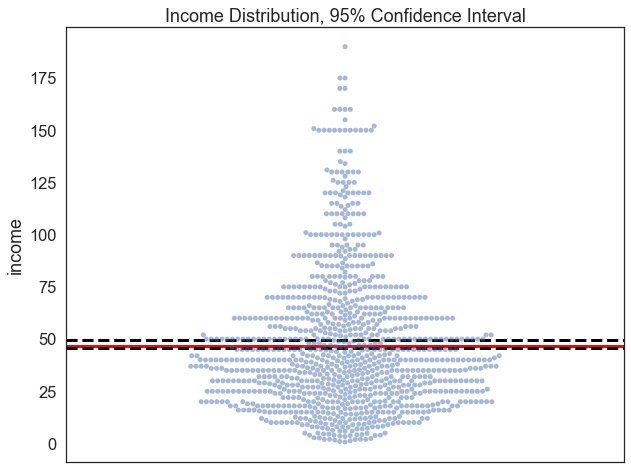
\includegraphics{notebooks/W03. Spatial Data_files/figure-pdf/cell-8-output-2.png}

}

\end{figure}

\hypertarget{my-first-map}{%
\section{My First Map}\label{my-first-map}}

The beauty of this data is that the data points have x and y values, so
plotting them as a scatter graph will give us out first approximation
(with caveats) of a map of the data:

\begin{Shaded}
\begin{Highlighting}[]
\NormalTok{tweets.plot(}
\NormalTok{    kind}\OperatorTok{=}\StringTok{\textquotesingle{}scatter\textquotesingle{}}\NormalTok{,}
\NormalTok{    x}\OperatorTok{=}\StringTok{\textquotesingle{}Lon\textquotesingle{}}\NormalTok{,}
\NormalTok{    y}\OperatorTok{=}\StringTok{\textquotesingle{}Lat\textquotesingle{}}\NormalTok{,}
\NormalTok{    title}\OperatorTok{=}\StringTok{"Location of Tweets"}\NormalTok{)}
\NormalTok{plt.xlabel(}\StringTok{"Longitude [degrees]"}\NormalTok{)}
\NormalTok{plt.ylabel(}\StringTok{"Latitude [degrees]"}\NormalTok{)}
\end{Highlighting}
\end{Shaded}

\begin{verbatim}
Text(0, 0.5, 'Latitude [degrees]')
\end{verbatim}

\begin{figure}[H]

{\centering 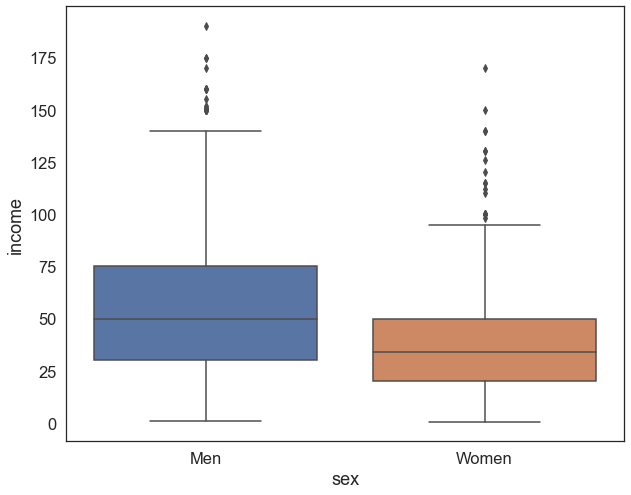
\includegraphics{notebooks/W03. Spatial Data_files/figure-pdf/cell-9-output-2.png}

}

\end{figure}

Notice that we've laid out the code so it's easier to see the multiple
arguments in plot() - this is just the same as:

\begin{Shaded}
\begin{Highlighting}[]
\NormalTok{tweets.plot(kind}\OperatorTok{=}\StringTok{\textquotesingle{}scatter\textquotesingle{}}\NormalTok{,x}\OperatorTok{=}\StringTok{\textquotesingle{}Lon\textquotesingle{}}\NormalTok{,y}\OperatorTok{=}\StringTok{\textquotesingle{}Lat\textquotesingle{}}\NormalTok{, title}\OperatorTok{=}\StringTok{"Location of Tweets"}\NormalTok{)}
\NormalTok{plt.xlabel(}\StringTok{"Longitude [degrees]"}\NormalTok{)}
\NormalTok{plt.ylabel(}\StringTok{"Latitude [degrees]"}\NormalTok{)}
\end{Highlighting}
\end{Shaded}

\begin{verbatim}
Text(0, 0.5, 'Latitude [degrees]')
\end{verbatim}

\begin{figure}[H]

{\centering 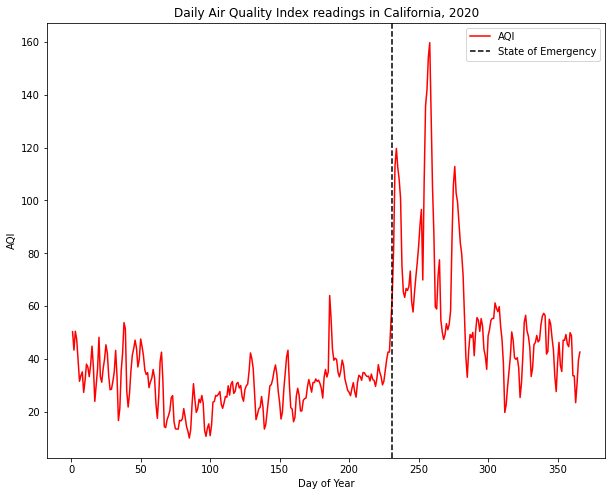
\includegraphics{notebooks/W03. Spatial Data_files/figure-pdf/cell-10-output-2.png}

}

\end{figure}

\begin{Shaded}
\begin{Highlighting}[]
\ImportTok{import}\NormalTok{ folium}
\end{Highlighting}
\end{Shaded}

\hypertarget{exercise-7}{%
\section{Exercise}\label{exercise-7}}

Change the style of the above map using the optional arguments:

\begin{itemize}
\tightlist
\item
  \emph{alpha = }: to set the opacity - 1 being opaque and 0 being
  transparent. Set the transparecny so that you can see busy areas
  \emph{and} individual points
\item
  \emph{color=}: to set the colo\emph{u}r to `red'
\item
  \emph{s=}: so set the point size to 50
\end{itemize}

So we have something that looks a bit like a heat map, and even looks a
bit Gaussian. Let's see what a histogram of this data looks like:

\begin{Shaded}
\begin{Highlighting}[]
\NormalTok{tweets[}\StringTok{\textquotesingle{}Lat\textquotesingle{}}\NormalTok{].hist(bins }\OperatorTok{=} \DecValTok{50}\NormalTok{)}
\NormalTok{plt.xlabel(}\StringTok{"Latitude [degrees]"}\NormalTok{)}
\NormalTok{plt.ylabel(}\StringTok{"Number of Tweets"}\NormalTok{)}
\end{Highlighting}
\end{Shaded}

\begin{verbatim}
Text(0, 0.5, 'Number of Tweets')
\end{verbatim}

\begin{figure}[H]

{\centering 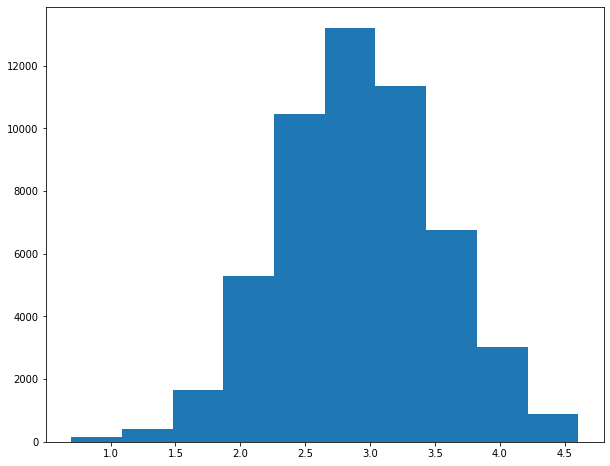
\includegraphics{notebooks/W03. Spatial Data_files/figure-pdf/cell-12-output-2.png}

}

\end{figure}

\begin{Shaded}
\begin{Highlighting}[]
\NormalTok{ax }\OperatorTok{=}\NormalTok{ tweets[}\StringTok{\textquotesingle{}Lon\textquotesingle{}}\NormalTok{].hist(bins}\OperatorTok{=}\DecValTok{50}\NormalTok{)}
\NormalTok{plt.xlabel(}\StringTok{"Longitude [degrees]"}\NormalTok{)}
\NormalTok{ax.set\_ylabel(}\StringTok{"Number of Tweets"}\NormalTok{)}
\end{Highlighting}
\end{Shaded}

\begin{verbatim}
Text(0, 0.5, 'Number of Tweets')
\end{verbatim}

\begin{figure}[H]

{\centering \includegraphics{notebooks/W03. Spatial Data_files/figure-pdf/cell-13-output-2.png}

}

\end{figure}

\hypertarget{the-naivest-projection}{%
\section{The Naivest Projection}\label{the-naivest-projection}}

The above tweet plot implicitly uses the \emph{equirectangular}
projection, which maps longitude onto the x axis, and latitude onto the
y axis. What is the problem with this ?

Projection is hugely complex and mathematically fiddly - luckily, we'll
be working with packages which mostly do the heavy lifting for us. It's
still worth thinking about projection a bit, as the process of taking
points on a sphere and translating that to a flat surface is never a
perfect one.

If we look at the picture below, then clearly the distance between \(p\)
and \(q\) is the length of the curve on the sphere rather than the
straight line between them. The closer \(p\) and \(q\) are the more the
distance is like a straight line, and we can use a \emph{linear mapping}
- i.e.~the x coordinate is a linear function of lon, and the y axis is a
linear function of latitude.

\hypertarget{extension-not-so-great-circles}{%
\section{Extension: Not-so-great
circles}\label{extension-not-so-great-circles}}

Calculating great circle distances is the ``real'' way of figuring out
the distance between two points on a sphere is fairly complex.
Thankfully, there's a small angle approximation.

If the two points (1 and 2) have latitudes \(\phi_1\) and \(\phi_2\) and
longitudes \(\lambda_1\) and \(\lambda_2\), then let
\(\Delta\phi = \phi_1 - \phi_2\) and
\(\Delta\lambda = \lambda_1 - \lambda_2\) , where
\((\phi_1,\lambda_1) ,(\phi_2,\lambda_2)\) are two points given in
(latitude, longitude).

If \(\Delta\phi\) and \(\Delta\lambda\) are small enough, you can
calculate the distance \(D\) with :

\[D = R \sqrt{(\Delta\phi)^2+(cos(\bar{\phi})\Delta\lambda)^2}\]

where \(\bar{\phi}\) is the mean latitude of the two points,
\(\frac{1}{2}(\phi_1+\phi_2)\), and R is the radius of the earth.

How small is small enough if we want to use this approximation? Well, it
depends on how much error you want to incur. But generally if the angles
are much less than one radian, you'll incur small errors. Radians, you
say? Yes, everything in the above equations assumes angles are expressed
in radians. 1 radian is about 57 degrees, but there are more precise
definitions, and python has a utility function for converting between
the two.

For reference, the errors accumulated over the size of London are tens
of metres.

\hypertarget{british-values}{%
\section{British Values}\label{british-values}}

The British National Grid provides projected values in metres, so we can
get by without doing projections ``on the fly'' just yet. If we plot
these values, it will look pretty similar, for the reasons outlined
above - over the few km of London, most projection methods are quite
close to the linear mapping we've done.

\begin{Shaded}
\begin{Highlighting}[]
\NormalTok{ax }\OperatorTok{=}\NormalTok{ tweets.plot(}
\NormalTok{    kind}\OperatorTok{=}\StringTok{\textquotesingle{}scatter\textquotesingle{}}\NormalTok{,}
\NormalTok{    x}\OperatorTok{=}\StringTok{\textquotesingle{}OSGB\_Lon\textquotesingle{}}\NormalTok{,}
\NormalTok{    y}\OperatorTok{=}\StringTok{\textquotesingle{}OSGB\_Lat\textquotesingle{}}\NormalTok{,}
\NormalTok{    title}\OperatorTok{=}\StringTok{"Location of Tweets"}\NormalTok{)}
\NormalTok{ax.set\_xlabel(}\StringTok{"projected Longitude"}\NormalTok{)}
\NormalTok{ax.set\_ylabel(}\StringTok{"projected Latitude"}\NormalTok{)}
\end{Highlighting}
\end{Shaded}

\begin{verbatim}
Text(0, 0.5, 'projected Latitude')
\end{verbatim}

\begin{figure}[H]

{\centering 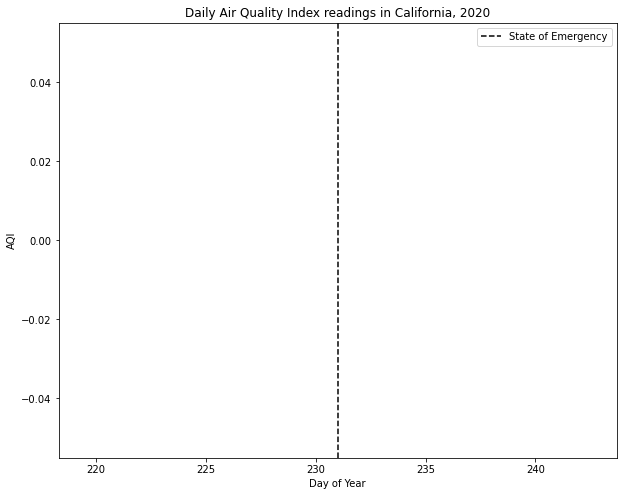
\includegraphics{notebooks/W03. Spatial Data_files/figure-pdf/cell-15-output-2.png}

}

\end{figure}

\hypertarget{exercise-describing-the-data}{%
\section{Exercise: Describing the
Data}\label{exercise-describing-the-data}}

\begin{enumerate}
\def\labelenumi{\arabic{enumi})}
\item
  Find the data centroid (lat, lon)
\item
  Calculate the x, y and total extent of the data, in km (or miles).
  (Use the projected {[}OSGB{]} data for that.)
\end{enumerate}

Hint: use commands which capture the maximum, minimum and mean of the
data - describe() is a useful one here.

\hypertarget{exercise-8}{%
\section{Exercise}\label{exercise-8}}

How might we go about calculating the geographical extent which
contained 95\% of tweets? Assuming the distribution is Gaussian in both
variables, estimate a) the latitude the limits which contain 95\% of
tweets, b) the longitude limits which contain 95\% of tweets. Then c)
and add lines showing these limits to the tweet graph and d) save the
figure as an image using plt.savefig(\emph{filename}).

What proportion of tweets is held within this box?

How do you think the following elements influence the above result?

\begin{itemize}
\item
  The 2D nature of the data
\item
  Asymmetry of the Gaussian (i.e.~if \(\sigma_x \neq \sigma_y\))
\item
  Whether the data is Gaussian!
\item
  What other approaches could you take with this data?
\end{itemize}

\hypertarget{working-in-2d}{%
\section{Working in 2D}\label{working-in-2d}}

It's clear that we can learn from 1D about how we can approach 2D data.
But there are limitations, and treating 2D as two sets of 1D data
doesn't work for everything. We need to find ways to carry out
histograms and other aggregations in 2D - and the first of these is
hexbinning.

\hypertarget{hexbinning}{%
\section{Hexbinning}\label{hexbinning}}

We can also use a
\href{http://pandas-docs.github.io/pandas-docs-travis/visualization.html\#hexagonal-bin-plot}{hexbin
clustering} method, which is similar to binning in a histogram, the more
points we have in hexbin the warmer the color. Here, we count the number
data points in each hexagons, in the same way that we count the number
of data in each bin for 1D data

Luckily, the code is very easy to execute, and requires only small
changes:

\begin{Shaded}
\begin{Highlighting}[]
\NormalTok{ax }\OperatorTok{=}\NormalTok{ tweets.plot(}
\NormalTok{    kind}\OperatorTok{=}\StringTok{\textquotesingle{}hexbin\textquotesingle{}}\NormalTok{,}
\NormalTok{    x}\OperatorTok{=}\StringTok{\textquotesingle{}OSGB\_Lon\textquotesingle{}}\NormalTok{, y}\OperatorTok{=}\StringTok{\textquotesingle{}OSGB\_Lat\textquotesingle{}}\NormalTok{,}
\NormalTok{    gridsize}\OperatorTok{=}\DecValTok{50}\NormalTok{,}
\NormalTok{    title}\OperatorTok{=}\StringTok{"Tweet Density (Hex Bin)"}\NormalTok{,}
\NormalTok{    cmap}\OperatorTok{=}\StringTok{\textquotesingle{}coolwarm\textquotesingle{}}\NormalTok{,}
\NormalTok{    )}
\NormalTok{plt.xlabel(}\StringTok{"projected Longitude"}\NormalTok{)}
\NormalTok{plt.ylabel(}\StringTok{"projected Latitude"}\NormalTok{)}
\end{Highlighting}
\end{Shaded}

\begin{verbatim}
Text(0, 0.5, 'projected Latitude')
\end{verbatim}

\begin{figure}[H]

{\centering \includegraphics{notebooks/W03. Spatial Data_files/figure-pdf/cell-18-output-2.png}

}

\end{figure}

Possible values are: Spectral, summer, coolwarm, Wistia\_r, pink\_r,
Set1, Set2, Set3, brg\_r, Dark2, prism, PuOr\_r, afmhot\_r, terrain\_r,
PuBuGn\_r, RdPu, gist\_ncar\_r, gist\_yarg\_r, Dark2\_r, YlGnBu, RdYlBu,
hot\_r, gist\_rainbow\_r, gist\_stern, PuBu\_r, cool\_r, cool, gray,
copper\_r, Greens\_r, GnBu, gist\_ncar, spring\_r, gist\_rainbow,
gist\_heat\_r, Wistia, OrRd\_r, CMRmap, bone, gist\_stern\_r, RdYlGn,
Pastel2\_r, spring, terrain, YlOrRd\_r, Set2\_r, winter\_r, PuBu,
RdGy\_r, spectral, rainbow, flag\_r, jet\_r, RdPu\_r, gist\_yarg, BuGn,
Paired\_r, hsv\_r, bwr, cubehelix, Greens, PRGn, gist\_heat,
spectral\_r, Paired, hsv, Oranges\_r, prism\_r, Pastel2, Pastel1\_r,
Pastel1, gray\_r, jet, Spectral\_r, gnuplot2\_r, gist\_earth, YlGnBu\_r,
copper, gist\_earth\_r, Set3\_r, OrRd, gnuplot\_r, ocean\_r, brg,
gnuplot2, PuRd\_r, bone\_r, BuPu, Oranges, RdYlGn\_r, PiYG, CMRmap\_r,
YlGn, binary\_r, gist\_gray\_r, Accent, BuPu\_r, gist\_gray, flag,
bwr\_r, RdBu\_r, BrBG, Reds, Set1\_r, summer\_r, GnBu\_r, BrBG\_r,
Reds\_r, RdGy, PuRd, Accent\_r, Blues, autumn\_r, autumn, cubehelix\_r,
nipy\_spectral\_r, ocean, PRGn\_r, Greys\_r, pink, binary, winter,
gnuplot, RdYlBu\_r, hot, YlOrBr, coolwarm\_r, rainbow\_r, Purples\_r,
PiYG\_r, YlGn\_r, Blues\_r, YlOrBr\_r, seismic, Purples, seismic\_r,
RdBu, Greys, BuGn\_r, YlOrRd, PuOr, PuBuGn, nipy\_spectral, afmhot

\hypertarget{extension-splitting-mapping-data-by-time}{%
\section{Extension: Splitting Mapping Data by
Time}\label{extension-splitting-mapping-data-by-time}}

In the next section, we use both space and time to show different
geographical distributions at different times. We'll select on index,
splitting the dataset in two.

\begin{Shaded}
\begin{Highlighting}[]
\NormalTok{early }\OperatorTok{=}\NormalTok{ tweets[:}\DecValTok{750}\NormalTok{]}
\NormalTok{late }\OperatorTok{=}\NormalTok{ tweets[}\DecValTok{750}\NormalTok{:}\BuiltInTok{len}\NormalTok{(tweets)]}
\end{Highlighting}
\end{Shaded}

\begin{Shaded}
\begin{Highlighting}[]
\NormalTok{early.head()}
\end{Highlighting}
\end{Shaded}

\begin{longtable}[]{@{}llllllll@{}}
\toprule()
& id & dateT & name & Lat & Lon & OSGB\_Lon & OSGB\_Lat \\
\midrule()
\endhead
0 & 15 & 2010-04-28 15:03:00 & MrFlexDot (Felix Tekyi) & 51.682488 &
-0.045406 & 535225.835914 & 200000.009703 \\
1 & 19 & 2010-04-28 15:03:00 & genyfrmdablck (geny ) & 51.539869 &
-0.135413 & 529408.436064 & 183977.283107 \\
2 & 26 & 2010-04-28 15:03:00 & makapala (Dave Woodford) & 51.459499 &
-0.036607 & 536499.925360 & 175219.249296 \\
3 & 31 & 2010-04-28 15:03:00 & JayVades (JayVades) & 51.518075 &
0.024400 & 540557.757933 & 181848.336146 \\
4 & 38 & 2010-04-28 15:03:00 & CatchAChoo (Jimmy Choo) & 51.510000 &
-0.217000 & 523831.617422 & 180514.655542 \\
\bottomrule()
\end{longtable}

\begin{Shaded}
\begin{Highlighting}[]
\NormalTok{late.head()}
\end{Highlighting}
\end{Shaded}

\begin{longtable}[]{@{}llllllll@{}}
\toprule()
& id & dateT & name & Lat & Lon & OSGB\_Lon & OSGB\_Lat \\
\midrule()
\endhead
750 & 4535 & 2010-04-28 15:23:00 & nadyavr (Nadya Valenza R) & 51.520975
& -0.049123 & 535448.286382 & 182032.267058 \\
751 & 4539 & 2010-04-28 15:23:00 & janasanchez (Jana Sanchez) &
51.481550 & -0.188767 & 525869.039823 & 177399.005684 \\
752 & 4543 & 2010-04-28 15:23:00 & BUMSHA (Bunmi Olowoporoku?) &
51.663310 & -0.068944 & 533655.100907 & 197824.013895 \\
753 & 4556 & 2010-04-28 15:23:00 & MrBell74 (Colin Bell) & 51.467061 &
0.201290 & 553000.411504 & 176530.046180 \\
754 & 4569 & 2010-04-28 15:23:00 & DineHard (Neil Davey) & 51.470925 &
-0.237811 & 522492.091850 & 176134.358324 \\
\bottomrule()
\end{longtable}

\hypertarget{exercise-9}{%
\section{Exercise}\label{exercise-9}}

Plot both sets of tweets onto the same axes so they can be compared. Try
and make your plot look like the image below.

We can visually inspect the spatial plots of the two time frames using
hexbin plots; in this case there's not much to see\ldots{}

\begin{Shaded}
\begin{Highlighting}[]
\NormalTok{ax }\OperatorTok{=}\NormalTok{ early.plot(}
\NormalTok{    kind}\OperatorTok{=}\StringTok{\textquotesingle{}hexbin\textquotesingle{}}\NormalTok{,}
\NormalTok{    x}\OperatorTok{=}\StringTok{\textquotesingle{}OSGB\_Lon\textquotesingle{}}\NormalTok{, }
\NormalTok{    y}\OperatorTok{=}\StringTok{\textquotesingle{}OSGB\_Lat\textquotesingle{}}\NormalTok{,}
\NormalTok{    gridsize}\OperatorTok{=}\DecValTok{50}\NormalTok{,}
\NormalTok{    title}\OperatorTok{=}\StringTok{"Tweet Density (Hex Bin)"}\NormalTok{,}
\NormalTok{    cmap}\OperatorTok{=}\StringTok{\textquotesingle{}coolwarm\textquotesingle{}}\NormalTok{,}
\NormalTok{    )}
\NormalTok{plt.xlabel(}\StringTok{"projected Longitude"}\NormalTok{)}
\NormalTok{plt.ylabel(}\StringTok{"projected Latitude"}\NormalTok{)}
\end{Highlighting}
\end{Shaded}

\begin{verbatim}
Text(0, 0.5, 'projected Latitude')
\end{verbatim}

\begin{figure}[H]

{\centering \includegraphics{notebooks/W03. Spatial Data_files/figure-pdf/cell-24-output-2.png}

}

\end{figure}

\begin{Shaded}
\begin{Highlighting}[]
\NormalTok{ax }\OperatorTok{=}\NormalTok{ late.plot(}
\NormalTok{    kind}\OperatorTok{=}\StringTok{\textquotesingle{}hexbin\textquotesingle{}}\NormalTok{,}
\NormalTok{    x}\OperatorTok{=}\StringTok{\textquotesingle{}OSGB\_Lon\textquotesingle{}}\NormalTok{, }
\NormalTok{    y}\OperatorTok{=}\StringTok{\textquotesingle{}OSGB\_Lat\textquotesingle{}}\NormalTok{,}
\NormalTok{    gridsize}\OperatorTok{=}\DecValTok{50}\NormalTok{,}
\NormalTok{    title}\OperatorTok{=}\StringTok{"Tweet Density (Hex Bin)"}\NormalTok{,}
\NormalTok{    cmap}\OperatorTok{=}\StringTok{\textquotesingle{}coolwarm\textquotesingle{}}\NormalTok{,}
\NormalTok{    )}
\NormalTok{plt.xlabel(}\StringTok{"projected Longitude"}\NormalTok{)}
\NormalTok{plt.ylabel(}\StringTok{"projected Latitude"}\NormalTok{)}
\end{Highlighting}
\end{Shaded}

\begin{verbatim}
Text(0, 0.5, 'projected Latitude')
\end{verbatim}

\begin{figure}[H]

{\centering \includegraphics{notebooks/W03. Spatial Data_files/figure-pdf/cell-25-output-2.png}

}

\end{figure}

\bookmarksetup{startatroot}

\hypertarget{natural-language-processing}{%
\chapter{Natural Language
Processing}\label{natural-language-processing}}

\hypertarget{workshop-4-open-in-colab}{%
\section[\emph{Workshop 4} ]{\texorpdfstring{\emph{Workshop 4}
\href{https://colab.research.google.com/github/oballinger/QM2/blob/main/notebooks/W04.\%20Natural\%20Language\%20Processing.ipynb}{\protect
\includegraphics{notebooks/../colab-badge.png}}}{Workshop 4 Open In Colab}}\label{workshop-4-open-in-colab}}

Today we'll be using the \emph{Natural Language Tool Kit} package
\textbf{nltk}, which will allow us to split (clean) text into words,
parts of speech, and sentences, and plot word occurrence and frequency.

\textbf{Aims}

\begin{itemize}
\tightlist
\item
  to work with nltk and some standard corpus texts
\item
  to tokenise by word and sentence
\item
  to plot word occurrence and frequency
\item
  to filter by parts of speech
\end{itemize}

\hypertarget{downloading-the-data-2}{%
\section{Downloading the Data}\label{downloading-the-data-2}}

Let's grab the data we will need this week from our course website and
save it into our data folder. If you've not already created a data
folder then do so using the following command.

Don't worry if it generates an error, that means you've already got a
data folder.

\begin{Shaded}
\begin{Highlighting}[]
\CommentTok{\#Make a ./data directory}
\OperatorTok{!}\NormalTok{pip install nltk}
\OperatorTok{!}\NormalTok{mkdir data}
\end{Highlighting}
\end{Shaded}

\begin{verbatim}
Requirement already satisfied: nltk in /Users/ollieballinger/.pyenv/versions/3.9.5/lib/python3.9/site-packages (3.7)
Requirement already satisfied: click in /Users/ollieballinger/.pyenv/versions/3.9.5/lib/python3.9/site-packages (from nltk) (8.0.1)
Requirement already satisfied: joblib in /Users/ollieballinger/.pyenv/versions/3.9.5/lib/python3.9/site-packages (from nltk) (1.0.1)
Requirement already satisfied: regex>=2021.8.3 in /Users/ollieballinger/.pyenv/versions/3.9.5/lib/python3.9/site-packages (from nltk) (2022.9.13)
Requirement already satisfied: tqdm in /Users/ollieballinger/.pyenv/versions/3.9.5/lib/python3.9/site-packages (from nltk) (4.61.0)
WARNING: You are using pip version 21.1.2; however, version 22.2.2 is available.
You should consider upgrading via the '/Users/ollieballinger/.pyenv/versions/3.9.5/bin/python3.9 -m pip install --upgrade pip' command.
mkdir: data: File exists
\end{verbatim}

\begin{Shaded}
\begin{Highlighting}[]
\CommentTok{\#Make a ./data/wk7 directory}
\OperatorTok{!}\NormalTok{mkdir data}\OperatorTok{/}\NormalTok{wk7}

\CommentTok{\#Download the data into this directory}
\OperatorTok{!}\NormalTok{curl https:}\OperatorTok{//}\NormalTok{s3.eu}\OperatorTok{{-}}\NormalTok{west}\OperatorTok{{-}}\FloatTok{2.}\ErrorTok{amazonaws}\NormalTok{.com}\OperatorTok{/}\NormalTok{qm2}\OperatorTok{/}\NormalTok{wk7}\OperatorTok{/}\NormalTok{PanelA.txt }\OperatorTok{{-}}\NormalTok{o .}\OperatorTok{/}\NormalTok{data}\OperatorTok{/}\NormalTok{wk4}\OperatorTok{/}\NormalTok{PanelA.txt}
\OperatorTok{!}\NormalTok{curl https:}\OperatorTok{//}\NormalTok{s3.eu}\OperatorTok{{-}}\NormalTok{west}\OperatorTok{{-}}\FloatTok{2.}\ErrorTok{amazonaws}\NormalTok{.com}\OperatorTok{/}\NormalTok{qm2}\OperatorTok{/}\NormalTok{wk7}\OperatorTok{/}\NormalTok{PanelA2.txt }\OperatorTok{{-}}\NormalTok{o .}\OperatorTok{/}\NormalTok{data}\OperatorTok{/}\NormalTok{wk4}\OperatorTok{/}\NormalTok{PanelA2.txt}
\OperatorTok{!}\NormalTok{curl https:}\OperatorTok{//}\NormalTok{s3.eu}\OperatorTok{{-}}\NormalTok{west}\OperatorTok{{-}}\FloatTok{2.}\ErrorTok{amazonaws}\NormalTok{.com}\OperatorTok{/}\NormalTok{qm2}\OperatorTok{/}\NormalTok{wk7}\OperatorTok{/}\NormalTok{PanelB.txt }\OperatorTok{{-}}\NormalTok{o .}\OperatorTok{/}\NormalTok{data}\OperatorTok{/}\NormalTok{wk4}\OperatorTok{/}\NormalTok{PanelB.txt}
\OperatorTok{!}\NormalTok{curl https:}\OperatorTok{//}\NormalTok{s3.eu}\OperatorTok{{-}}\NormalTok{west}\OperatorTok{{-}}\FloatTok{2.}\ErrorTok{amazonaws}\NormalTok{.com}\OperatorTok{/}\NormalTok{qm2}\OperatorTok{/}\NormalTok{wk7}\OperatorTok{/}\NormalTok{PanelC.txt }\OperatorTok{{-}}\NormalTok{o .}\OperatorTok{/}\NormalTok{data}\OperatorTok{/}\NormalTok{wk4}\OperatorTok{/}\NormalTok{PanelC.txt}
\OperatorTok{!}\NormalTok{curl https:}\OperatorTok{//}\NormalTok{s3.eu}\OperatorTok{{-}}\NormalTok{west}\OperatorTok{{-}}\FloatTok{2.}\ErrorTok{amazonaws}\NormalTok{.com}\OperatorTok{/}\NormalTok{qm2}\OperatorTok{/}\NormalTok{wk7}\OperatorTok{/}\NormalTok{PanelD.txt }\OperatorTok{{-}}\NormalTok{o .}\OperatorTok{/}\NormalTok{data}\OperatorTok{/}\NormalTok{wk4}\OperatorTok{/}\NormalTok{PanelD.txt}
\end{Highlighting}
\end{Shaded}

\begin{verbatim}
mkdir: data/wk7: File exists
  % Total    % Received % Xferd  Average Speed   Time    Time     Time  Current
                                 Dload  Upload   Total   Spent    Left  Speed
100  6374  100  6374    0     0  87376      0 --:--:-- --:--:-- --:--:-- 92376
  % Total    % Received % Xferd  Average Speed   Time    Time     Time  Current
                                 Dload  Upload   Total   Spent    Left  Speed
100  4091  100  4091    0     0  36609      0 --:--:-- --:--:-- --:--:-- 39336
  % Total    % Received % Xferd  Average Speed   Time    Time     Time  Current
                                 Dload  Upload   Total   Spent    Left  Speed
100 10903  100 10903    0     0  63110      0 --:--:-- --:--:-- --:--:-- 64514
  % Total    % Received % Xferd  Average Speed   Time    Time     Time  Current
                                 Dload  Upload   Total   Spent    Left  Speed
100  8140  100  8140    0     0  32892      0 --:--:-- --:--:-- --:--:-- 336306
  % Total    % Received % Xferd  Average Speed   Time    Time     Time  Current
                                 Dload  Upload   Total   Spent    Left  Speed
100  5801  100  5801    0     0  45085      0 --:--:-- --:--:-- --:--:-- 46782
\end{verbatim}

\begin{Shaded}
\begin{Highlighting}[]
\ImportTok{import}\NormalTok{ pylab}
\OperatorTok{\%}\NormalTok{matplotlib inline}
\NormalTok{pylab.rcParams[}\StringTok{\textquotesingle{}figure.figsize\textquotesingle{}}\NormalTok{] }\OperatorTok{=}\NormalTok{ (}\FloatTok{10.}\NormalTok{, }\FloatTok{8.}\NormalTok{)}
\end{Highlighting}
\end{Shaded}

\hypertarget{dirty-words}{%
\section{Dirty Words}\label{dirty-words}}

Text often comes `unclean' either containing tags such as HTML (or XML),
or has other issues, but fortunately we will be using `clean' sources,
at least initially. Be cautious when committing to a text analysis
project - you may spend a great deal of time tidying up your text.

The kind of analysis we will be doing reqires \emph{tokenizing} a text,
and \emph{tagging} individual words. Tokenizing means splitting the text
into individul sentences or individual words, while tagging means
classifying each word according to a POS (Parts Of Speech)
classification.

\hypertarget{the-castle-of-aaargh}{%
\section{The Castle of Aaargh}\label{the-castle-of-aaargh}}

We will first experiment with nltk and its built in corpus texts. We'll
work with some Monty Python, beloved of comedy bores for half a century

\hypertarget{setup}{%
\section{Setup}\label{setup}}

\begin{itemize}
\tightlist
\item
  install nltk through package manager, or the command line
\item
  import nltk
\item
  type nltk.download(`book'). This will automatically download the books
  into our workspace
\end{itemize}

\begin{Shaded}
\begin{Highlighting}[]
\CommentTok{\#nltk: natural language processing toolkit}
\ImportTok{import}\NormalTok{ nltk}
\end{Highlighting}
\end{Shaded}

\begin{Shaded}
\begin{Highlighting}[]
\CommentTok{\#Download the sample books}
\NormalTok{nltk.download(}\StringTok{\textquotesingle{}book\textquotesingle{}}\NormalTok{)}
\end{Highlighting}
\end{Shaded}

\begin{verbatim}
[nltk_data] Downloading collection 'book'
[nltk_data]    | 
[nltk_data]    | Downloading package abc to
[nltk_data]    |     /Users/ollieballinger/nltk_data...
[nltk_data]    |   Package abc is already up-to-date!
[nltk_data]    | Downloading package brown to
[nltk_data]    |     /Users/ollieballinger/nltk_data...
[nltk_data]    |   Package brown is already up-to-date!
[nltk_data]    | Downloading package chat80 to
[nltk_data]    |     /Users/ollieballinger/nltk_data...
[nltk_data]    |   Package chat80 is already up-to-date!
[nltk_data]    | Downloading package cmudict to
[nltk_data]    |     /Users/ollieballinger/nltk_data...
[nltk_data]    |   Package cmudict is already up-to-date!
[nltk_data]    | Downloading package conll2000 to
[nltk_data]    |     /Users/ollieballinger/nltk_data...
[nltk_data]    |   Package conll2000 is already up-to-date!
[nltk_data]    | Downloading package conll2002 to
[nltk_data]    |     /Users/ollieballinger/nltk_data...
[nltk_data]    |   Package conll2002 is already up-to-date!
[nltk_data]    | Downloading package dependency_treebank to
[nltk_data]    |     /Users/ollieballinger/nltk_data...
[nltk_data]    |   Package dependency_treebank is already up-to-date!
[nltk_data]    | Downloading package genesis to
[nltk_data]    |     /Users/ollieballinger/nltk_data...
[nltk_data]    |   Package genesis is already up-to-date!
[nltk_data]    | Downloading package gutenberg to
[nltk_data]    |     /Users/ollieballinger/nltk_data...
[nltk_data]    |   Package gutenberg is already up-to-date!
[nltk_data]    | Downloading package ieer to
[nltk_data]    |     /Users/ollieballinger/nltk_data...
[nltk_data]    |   Package ieer is already up-to-date!
[nltk_data]    | Downloading package inaugural to
[nltk_data]    |     /Users/ollieballinger/nltk_data...
[nltk_data]    |   Package inaugural is already up-to-date!
[nltk_data]    | Downloading package movie_reviews to
[nltk_data]    |     /Users/ollieballinger/nltk_data...
[nltk_data]    |   Package movie_reviews is already up-to-date!
[nltk_data]    | Downloading package nps_chat to
[nltk_data]    |     /Users/ollieballinger/nltk_data...
[nltk_data]    |   Package nps_chat is already up-to-date!
[nltk_data]    | Downloading package names to
[nltk_data]    |     /Users/ollieballinger/nltk_data...
[nltk_data]    |   Package names is already up-to-date!
[nltk_data]    | Downloading package ppattach to
[nltk_data]    |     /Users/ollieballinger/nltk_data...
[nltk_data]    |   Package ppattach is already up-to-date!
[nltk_data]    | Downloading package reuters to
[nltk_data]    |     /Users/ollieballinger/nltk_data...
[nltk_data]    |   Package reuters is already up-to-date!
[nltk_data]    | Downloading package senseval to
[nltk_data]    |     /Users/ollieballinger/nltk_data...
[nltk_data]    |   Package senseval is already up-to-date!
[nltk_data]    | Downloading package state_union to
[nltk_data]    |     /Users/ollieballinger/nltk_data...
[nltk_data]    |   Package state_union is already up-to-date!
[nltk_data]    | Downloading package stopwords to
[nltk_data]    |     /Users/ollieballinger/nltk_data...
[nltk_data]    |   Package stopwords is already up-to-date!
[nltk_data]    | Downloading package swadesh to
[nltk_data]    |     /Users/ollieballinger/nltk_data...
[nltk_data]    |   Package swadesh is already up-to-date!
[nltk_data]    | Downloading package timit to
[nltk_data]    |     /Users/ollieballinger/nltk_data...
[nltk_data]    |   Package timit is already up-to-date!
[nltk_data]    | Downloading package treebank to
[nltk_data]    |     /Users/ollieballinger/nltk_data...
[nltk_data]    |   Package treebank is already up-to-date!
[nltk_data]    | Downloading package toolbox to
[nltk_data]    |     /Users/ollieballinger/nltk_data...
[nltk_data]    |   Package toolbox is already up-to-date!
[nltk_data]    | Downloading package udhr to
[nltk_data]    |     /Users/ollieballinger/nltk_data...
[nltk_data]    |   Package udhr is already up-to-date!
[nltk_data]    | Downloading package udhr2 to
[nltk_data]    |     /Users/ollieballinger/nltk_data...
[nltk_data]    |   Package udhr2 is already up-to-date!
[nltk_data]    | Downloading package unicode_samples to
[nltk_data]    |     /Users/ollieballinger/nltk_data...
[nltk_data]    |   Package unicode_samples is already up-to-date!
[nltk_data]    | Downloading package webtext to
[nltk_data]    |     /Users/ollieballinger/nltk_data...
[nltk_data]    |   Package webtext is already up-to-date!
[nltk_data]    | Downloading package wordnet to
[nltk_data]    |     /Users/ollieballinger/nltk_data...
[nltk_data]    |   Package wordnet is already up-to-date!
[nltk_data]    | Downloading package wordnet_ic to
[nltk_data]    |     /Users/ollieballinger/nltk_data...
[nltk_data]    |   Package wordnet_ic is already up-to-date!
[nltk_data]    | Downloading package words to
[nltk_data]    |     /Users/ollieballinger/nltk_data...
[nltk_data]    |   Package words is already up-to-date!
[nltk_data]    | Downloading package maxent_treebank_pos_tagger to
[nltk_data]    |     /Users/ollieballinger/nltk_data...
[nltk_data]    |   Package maxent_treebank_pos_tagger is already up-
[nltk_data]    |       to-date!
[nltk_data]    | Downloading package maxent_ne_chunker to
[nltk_data]    |     /Users/ollieballinger/nltk_data...
[nltk_data]    |   Package maxent_ne_chunker is already up-to-date!
[nltk_data]    | Downloading package universal_tagset to
[nltk_data]    |     /Users/ollieballinger/nltk_data...
[nltk_data]    |   Package universal_tagset is already up-to-date!
[nltk_data]    | Downloading package punkt to
[nltk_data]    |     /Users/ollieballinger/nltk_data...
[nltk_data]    |   Package punkt is already up-to-date!
[nltk_data]    | Downloading package book_grammars to
[nltk_data]    |     /Users/ollieballinger/nltk_data...
[nltk_data]    |   Package book_grammars is already up-to-date!
[nltk_data]    | Downloading package city_database to
[nltk_data]    |     /Users/ollieballinger/nltk_data...
[nltk_data]    |   Package city_database is already up-to-date!
[nltk_data]    | Downloading package tagsets to
[nltk_data]    |     /Users/ollieballinger/nltk_data...
[nltk_data]    |   Package tagsets is already up-to-date!
[nltk_data]    | Downloading package panlex_swadesh to
[nltk_data]    |     /Users/ollieballinger/nltk_data...
[nltk_data]    |   Package panlex_swadesh is already up-to-date!
[nltk_data]    | Downloading package averaged_perceptron_tagger to
[nltk_data]    |     /Users/ollieballinger/nltk_data...
[nltk_data]    |   Package averaged_perceptron_tagger is already up-
[nltk_data]    |       to-date!
[nltk_data]    | 
[nltk_data]  Done downloading collection book
\end{verbatim}

\begin{verbatim}
True
\end{verbatim}

Now, we import the sample texts. You'll notice that text6 is ``Monty
Python and the Holy Grail'', as promised. Presumably this was compiled
pre-\emph{Spamalot}.

\begin{Shaded}
\begin{Highlighting}[]
\CommentTok{\#Import all features from nltk.book}
\ImportTok{from}\NormalTok{ nltk.book }\ImportTok{import} \OperatorTok{*}
\end{Highlighting}
\end{Shaded}

Let's look at the object text6; we can look at the first few words..

\begin{Shaded}
\begin{Highlighting}[]
\CommentTok{\#View the first ten words of text6}
\NormalTok{text6[}\DecValTok{1}\NormalTok{:}\DecValTok{10}\NormalTok{]}
\end{Highlighting}
\end{Shaded}

\begin{verbatim}
['1', ':', '[', 'wind', ']', '[', 'clop', 'clop', 'clop']
\end{verbatim}

Which are presumably stage directions rather than dialogue. How many
words/symbols are in the text?

\begin{Shaded}
\begin{Highlighting}[]
\CommentTok{\#View the length of the list}
\BuiltInTok{len}\NormalTok{(text6)}
\end{Highlighting}
\end{Shaded}

\begin{verbatim}
16967
\end{verbatim}

Bear in mind that a lot of the functions we will carry out rely on this
being a text object - we'll start to think about how we use free text
and convert it to a \textbf{Text} object later.

We can now start to do some slightly more sophisticated work; for
example, a dispersion plot to see where words appear. Let's give it a
few keywords that those familiar with \emph{\ldots The Holy Grail} might
recognise:

\begin{Shaded}
\begin{Highlighting}[]
\NormalTok{text6.dispersion\_plot([}\StringTok{\textquotesingle{}Grail\textquotesingle{}}\NormalTok{,}\StringTok{\textquotesingle{}rabbit\textquotesingle{}}\NormalTok{,}\StringTok{\textquotesingle{}Knights\textquotesingle{}}\NormalTok{,}\StringTok{\textquotesingle{}Ni\textquotesingle{}}\NormalTok{,}\StringTok{\textquotesingle{}castle\textquotesingle{}}\NormalTok{])}
\end{Highlighting}
\end{Shaded}

\begin{figure}[H]

{\centering \includegraphics{notebooks/W04. Natural Language Processing_files/figure-pdf/cell-10-output-1.png}

}

\end{figure}

And we can easily count \emph{how many} times a word appears.

\begin{Shaded}
\begin{Highlighting}[]
\NormalTok{text6.count(}\StringTok{\textquotesingle{}Ni\textquotesingle{}}\NormalTok{)}
\end{Highlighting}
\end{Shaded}

\begin{verbatim}
47
\end{verbatim}

Or the words which most commonly appear together:

\begin{Shaded}
\begin{Highlighting}[]
\NormalTok{text6.collocations()}
\end{Highlighting}
\end{Shaded}

\begin{verbatim}
BLACK KNIGHT; clop clop; HEAD KNIGHT; mumble mumble; Holy Grail;
squeak squeak; FRENCH GUARD; saw saw; Sir Robin; Run away; CARTOON
CHARACTER; King Arthur; Iesu domine; Pie Iesu; DEAD PERSON; Round
Table; clap clap; OLD MAN; dramatic chord; dona eis
\end{verbatim}

\hypertarget{exercise-from-hells-heart-i-stab-at-thee}{%
\section{Exercise: From Hell's Heart I Stab at
Thee}\label{exercise-from-hells-heart-i-stab-at-thee}}

From Moby Dick, find out - Where the narrator Ishmael, Captain Ahab and
his Nemesis are mentioned. When do each enter the story? Where do they
have most emphasis? - Which parts of the books appear to take place at
sea, and points where their ship is wrecked or sinking (spoilers) - two
significant places in the story (HINT: use collocations)

Let's now look at carrying out the full process of importing and working
with text data.

\hypertarget{making-an-impact}{%
\section{Making an IMPACT}\label{making-an-impact}}

As part of the REF2014 exercise, universities reported on the
\emph{Impact} their research activities had on the world. Their
\emph{Impact Case Studies} were subsequently made available by HEFCE.
What sort of information do they contain? How do universities frame
``impact''? All of this data is available via the REF website.

A little context: I've included examples from the four \emph{panels}
used by HEFCE. Broadly speaking, Panel A is health, bioscience and
medicine, B is physical science and engineering, C is social science,
and D is humanities - the full categories are visible here:
http://www.ref.ac.uk/panels/unitsofassessment/

Let's first look at random sample from Panel A:

\begin{Shaded}
\begin{Highlighting}[]
\CommentTok{\#Data path to file}
\NormalTok{data\_path }\OperatorTok{=} \StringTok{"./data/wk7/PanelA.txt"}

\ControlFlowTok{with} \BuiltInTok{open}\NormalTok{(data\_path) }\ImportTok{as} \BuiltInTok{file}\NormalTok{:}
\NormalTok{    data }\OperatorTok{=} \BuiltInTok{file}\NormalTok{.read()}
\BuiltInTok{print}\NormalTok{(data)}
\end{Highlighting}
\end{Shaded}

\begin{verbatim}
FileNotFoundError: [Errno 2] No such file or directory: './data/wk7/PanelA.txt'
\end{verbatim}

We could tokenize this into sentences:

\begin{Shaded}
\begin{Highlighting}[]
\NormalTok{sentences }\OperatorTok{=}\NormalTok{ nltk.sent\_tokenize(data)}
\NormalTok{sentences[}\DecValTok{1}\NormalTok{:}\DecValTok{5}\NormalTok{]}
\end{Highlighting}
\end{Shaded}

\begin{verbatim}
['Researchers developed a practice development framework for implementing and assessing the delivery of evidence-based practice in 82 UK health and social care units during the impact period.',
 'Benefits to staff include better communication and team structure.',
 'Benefits to patients include higher standards of cleanliness, privacy and dignity, as well as a decrease in length of hospital stays and appointment waiting times.',
 'Delivery has extended to cover entire NHS Trusts serving a resident population of over 3.5 million, social services departments and third sector organisations across the south of England and beyond.']
\end{verbatim}

Or into individual words; generally, it may be useful to retain
sentences, so we can see where two words are in the same sentence, for
example - but we'll be doing something simpler:

\begin{Shaded}
\begin{Highlighting}[]
\NormalTok{tokens }\OperatorTok{=}\NormalTok{ nltk.word\_tokenize(data)}
\end{Highlighting}
\end{Shaded}

\begin{Shaded}
\begin{Highlighting}[]
\NormalTok{tokens[}\DecValTok{1}\NormalTok{:}\DecValTok{20}\NormalTok{]}
\end{Highlighting}
\end{Shaded}

\begin{verbatim}
['*',
 '*',
 '*',
 '*',
 'title_inst_10000824-u_3-case_43396',
 '*',
 'UKPRN_10000824',
 '*',
 'uoa_3',
 '*',
 'ID_43396',
 '*',
 'panel_A',
 'Bournemouth',
 'University',
 '(',
 'BU',
 ')',
 'has']
\end{verbatim}

Tokenising is a process which has many subtleties and corner-cases, and
you may want to proceed in a more fine-grained way for some texts:

http://nltk.org/api/nltk.tokenize.html

Let's now convert this into a Text object, which will allow us to
analyse other aspects of the text. For example, we can look at
\textbf{collocations}, words which commonly appear together. This may
help to provide context.

\begin{Shaded}
\begin{Highlighting}[]
\NormalTok{simple\_text }\OperatorTok{=}\NormalTok{ nltk.Text(tokens)}
\NormalTok{simple\_text.collocations()}
\end{Highlighting}
\end{Shaded}

\begin{verbatim}
practice development; Foundation Trust; NHS Foundation; 3.5 million;
Poole Hospital; Trusts serving; resident population; social care;
Hospital NHS; waiting times; action plan; development process; patient
privacy; user journey; better communication; cultural change; visiting
times; team members; services departments; evidence-based practice
\end{verbatim}

We can create a dispersion plot - although in this case, it tells us a
limited amount\ldots{}

\begin{Shaded}
\begin{Highlighting}[]
\NormalTok{simple\_text.dispersion\_plot([}\StringTok{\textquotesingle{}NHS\textquotesingle{}}\NormalTok{, }\StringTok{\textquotesingle{}evidence\textquotesingle{}}\NormalTok{, }\StringTok{\textquotesingle{}practice\textquotesingle{}}\NormalTok{, }\StringTok{\textquotesingle{}Hospital\textquotesingle{}}\NormalTok{])}
\end{Highlighting}
\end{Shaded}

\begin{figure}[H]

{\centering \includegraphics{notebooks/W04. Natural Language Processing_files/figure-pdf/cell-18-output-1.png}

}

\end{figure}

Even from this, we get a sense of the work this unit does, and its
impacts on the world. But what are the most 20 common words used? To
find this out, we produce a \textbf{Freq}uency \textbf{Dist}ribution
(\emph{FreqDist}) object. This has an implicit loop - the \emph{for}
statement is telling python to look through all the words in `tokens'
and seeing how often they occur. The .lower() command converts them all
to lower case for comparison, so it will flag up upper \emph{and} lower
case occurrences of the word.

\begin{Shaded}
\begin{Highlighting}[]
\NormalTok{fd }\OperatorTok{=}\NormalTok{ nltk.FreqDist(word.lower() }\ControlFlowTok{for}\NormalTok{ word }\KeywordTok{in}\NormalTok{ tokens)}
\NormalTok{fd.plot(}\DecValTok{20}\NormalTok{)}
\end{Highlighting}
\end{Shaded}

\begin{figure}[H]

{\centering 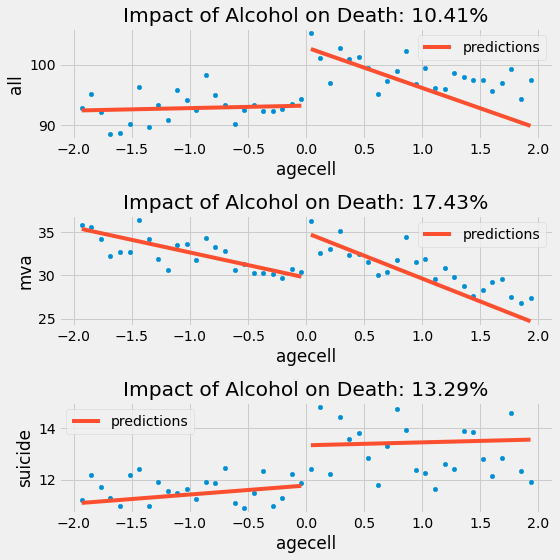
\includegraphics{notebooks/W04. Natural Language Processing_files/figure-pdf/cell-19-output-1.png}

}

\end{figure}

\begin{verbatim}
<AxesSubplot:xlabel='Samples', ylabel='Counts'>
\end{verbatim}

Not very helpful - this includes all kinds of junk, and tells us that
``and'' is very common. Not very interesting. Let's try a bit harder and
identify Parts of Speech.

\hypertarget{pos}{%
\section{POS}\label{pos}}

Parts of speech indicate whether something is a noun, a verb, adjective,
and so on. In nltk, we can use the \emph{pos\_tag} command, which will
identify which word belongs to which part of speech.

\begin{Shaded}
\begin{Highlighting}[]
\NormalTok{tagged }\OperatorTok{=}\NormalTok{ nltk.pos\_tag(tokens)}
\NormalTok{tagged[}\DecValTok{0}\NormalTok{:}\DecValTok{10}\NormalTok{]}
\end{Highlighting}
\end{Shaded}

\begin{verbatim}
[('*', 'JJ'),
 ('*', 'NNP'),
 ('*', 'NNP'),
 ('*', 'NNP'),
 ('*', 'NNP'),
 ('title_inst_10000824-u_3-case_43396', 'JJ'),
 ('*', 'NNP'),
 ('UKPRN_10000824', 'NNP'),
 ('*', 'NNP'),
 ('uoa_3', 'JJ')]
\end{verbatim}

`NNP' refers to Proper Noun, Singular; you can find the full list of
Parts of Speech here:
http://www.ling.upenn.edu/courses/Fall\_2003/ling001/penn\_treebank\_pos.html

\begin{Shaded}
\begin{Highlighting}[]
\NormalTok{permitted\_tags }\OperatorTok{=} \BuiltInTok{set}\NormalTok{([}
    \StringTok{\textquotesingle{}NN\textquotesingle{}}\NormalTok{,}
    \StringTok{\textquotesingle{}NNS\textquotesingle{}}
\NormalTok{])}
\end{Highlighting}
\end{Shaded}

\hypertarget{one-for-all}{%
\section{One FOR All}\label{one-for-all}}

We've so far managed to avoid this staple of programming, the FOR loop -
and we're not going to delve too deeply into it in the last class of
term. Of course, you probably came across FOR loops and IF statements
when you worked through the prerequisites for the module, but that feels
like a long time ago\ldots{}

We do use FOR and IF here, and it's worth understanding a bit about what
it means, even if you don't intend to use it a lot yourself. In the next
piece of code, we set up \emph{fd}, a new object which will record
frequency distribution information. Then we use a FOR loop

`for bit in tagged: \ldots'

This goes through every element of tagged one at a time - and each
element is called `bit' for the purposes of this loop. Then, for each
`bit', we check that it has one of the permitted tags, and make sure
it's at least 3 characters long - shorter words probably aren't all that
relevant in this case:

`if bit\href{http://www.literateprogramming.com/lpquotes.html}{1} in
permitted\_tags and len(bit{[}0{]})\textgreater2:'

note that the \emph{and} means both of these have to be true - if both
\emph{are} true, only then does the following statement execute:

`fd{[}bit{[}0{]}{]} = fd{[}bit{[}0{]}{]} + 1'

which increases the count for that word. So, this code increases the
count for a word iff (if and only if) its at least 3 characters long,
and it's of the correct tag (Noun, Singular or Plural).

\hypertarget{double-indentity}{%
\section{Double Indentity}\label{double-indentity}}

One final remark: we haven't dealt with \textbf{indents} much in python,
but indenting the code like below, after the for statement, and
\emph{again} after the if statement, is the way that python knows it's
dealing with a loop (for) and a conditional (if). It's also the way
python deals with defining new functions, but that's not something you
will need to do. This is just a pointer - if your code doesn't work,
check the colons are there (:) and the indenting is too.

On with the show - as promised, this creates a word frequency graph of
nouns:

\begin{Shaded}
\begin{Highlighting}[]
\NormalTok{fd }\OperatorTok{=}\NormalTok{ nltk.FreqDist()}

\ControlFlowTok{for}\NormalTok{ bit }\KeywordTok{in}\NormalTok{ tagged:}
    \ControlFlowTok{if}\NormalTok{ bit[}\DecValTok{1}\NormalTok{] }\KeywordTok{in}\NormalTok{ permitted\_tags }\KeywordTok{and} \BuiltInTok{len}\NormalTok{(bit[}\DecValTok{0}\NormalTok{])}\OperatorTok{\textgreater{}}\DecValTok{2}\NormalTok{:}
\NormalTok{        fd[bit[}\DecValTok{0}\NormalTok{]] }\OperatorTok{=}\NormalTok{ fd[bit[}\DecValTok{0}\NormalTok{]] }\OperatorTok{+} \DecValTok{1}
        
\NormalTok{fd.plot(}\DecValTok{20}\NormalTok{)}
\end{Highlighting}
\end{Shaded}

\begin{figure}[H]

{\centering 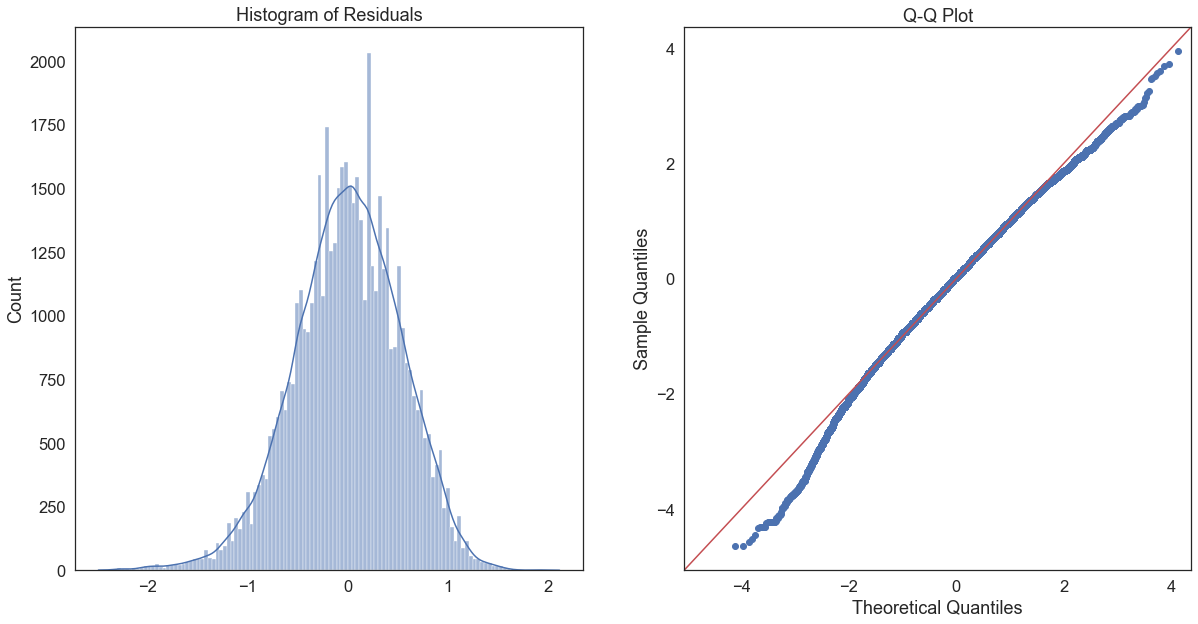
\includegraphics{notebooks/W04. Natural Language Processing_files/figure-pdf/cell-22-output-1.png}

}

\end{figure}

\begin{verbatim}
<AxesSubplot:xlabel='Samples', ylabel='Counts'>
\end{verbatim}

We start to get a sense of the impact - `care', `practice', and
`services' all feature heavily.

Let's now look at another randomly chosen example from Panel A:

\begin{Shaded}
\begin{Highlighting}[]
\NormalTok{data\_path }\OperatorTok{=} \StringTok{"./data/wk7/PanelA2.txt"}

\ControlFlowTok{with} \BuiltInTok{open}\NormalTok{(data\_path) }\ImportTok{as} \BuiltInTok{file}\NormalTok{:}
\NormalTok{    data }\OperatorTok{=} \BuiltInTok{file}\NormalTok{.read()}
\NormalTok{tokens }\OperatorTok{=}\NormalTok{ nltk.word\_tokenize(data)}
\NormalTok{simple\_text.collocations()}
\NormalTok{simple\_text }\OperatorTok{=}\NormalTok{ nltk.Text(tokens)}
\NormalTok{tagged }\OperatorTok{=}\NormalTok{ nltk.pos\_tag(tokens)}
\NormalTok{fd }\OperatorTok{=}\NormalTok{ nltk.FreqDist()}

\ControlFlowTok{for}\NormalTok{ bit }\KeywordTok{in}\NormalTok{ tagged:}
    \ControlFlowTok{if}\NormalTok{ bit[}\DecValTok{1}\NormalTok{] }\KeywordTok{in}\NormalTok{ permitted\_tags }\KeywordTok{and} \BuiltInTok{len}\NormalTok{(bit[}\DecValTok{0}\NormalTok{])}\OperatorTok{\textgreater{}}\DecValTok{2}\NormalTok{:}
\NormalTok{        fd[bit[}\DecValTok{0}\NormalTok{]] }\OperatorTok{=}\NormalTok{ fd[bit[}\DecValTok{0}\NormalTok{]] }\OperatorTok{+} \DecValTok{1}
        
\NormalTok{fd.plot(}\DecValTok{20}\NormalTok{)}
\end{Highlighting}
\end{Shaded}

\begin{verbatim}
practice development; Foundation Trust; NHS Foundation; 3.5 million;
Poole Hospital; Trusts serving; resident population; social care;
Hospital NHS; waiting times; action plan; development process; patient
privacy; user journey; better communication; cultural change; visiting
times; team members; services departments; evidence-based practice
\end{verbatim}

\begin{figure}[H]

{\centering \includegraphics{notebooks/W04. Natural Language Processing_files/figure-pdf/cell-23-output-2.png}

}

\end{figure}

\begin{verbatim}
<AxesSubplot:xlabel='Samples', ylabel='Counts'>
\end{verbatim}

A very different set of words, clearly geared towards language therapy,
and working directly with patients. Perhaps if we looked at the
\emph{slightly} less common words, we'd see links between these
submissions - for example, we see \emph{communication} appearing in
both. Not a huge surprise, if we're talking about public impact, but
students of the public role of the university might start to wonder
about the distinctions between \emph{communication} and
\emph{engagement}.

\hypertarget{exercise-10}{%
\section{Exercise}\label{exercise-10}}

Repeat this for the examples from Panels B, C and D - what trends and
keywords appear? What use do the collocations have? What do different
parts of speech (e.g.~verbs or proper nouns) tell you about the text?

If we wanted to analyse the sector as a whole, we would want to analyse
Impact statements en masse - and we would hope that this would draw out
links across differnt statements from different centres and
universities, and even in different panels.

\hypertarget{working-with-larger-text-datasets}{%
\section{Working with larger text
datasets}\label{working-with-larger-text-datasets}}

Working with larger text corpora starts to get slow. At this point, we
will look at a body of text we have previously tagged up. The file is
``The Nameless City'' by H. P. Lovecraft, a horror author from the early
20th century.

\begin{Shaded}
\begin{Highlighting}[]
\ImportTok{import}\NormalTok{ pickle}
\ImportTok{import}\NormalTok{ requests}
\ImportTok{from}\NormalTok{ urllib.request }\ImportTok{import}\NormalTok{ urlopen}
\end{Highlighting}
\end{Shaded}

This may take a little while - so wait for the task to run:

\begin{Shaded}
\begin{Highlighting}[]
\CommentTok{\# Loading the tokenized and tagged file. }
\NormalTok{tagged }\OperatorTok{=}\NormalTok{ pickle.load(urlopen(}\StringTok{"https://s3.eu{-}west{-}2.amazonaws.com/qm2/wk7/lovecraft\_tagged.pickle"}\NormalTok{), encoding}\OperatorTok{=}\StringTok{\textquotesingle{}latin1\textquotesingle{}}\NormalTok{)}

\CommentTok{\#How many sentences do we have?}
\BuiltInTok{len}\NormalTok{(tagged)}
\end{Highlighting}
\end{Shaded}

\begin{verbatim}
18513
\end{verbatim}

This is tokenised by sentence - and there are 18,513 of them. That would
have taken a long time to tag up. If you're interested, this is how you
take a set of \emph{sentences} and tag them with Part of Speech:

\begin{Shaded}
\begin{Highlighting}[]
\NormalTok{exampleSentences }\OperatorTok{=}\NormalTok{ nltk.sent\_tokenize(data)}
  
\NormalTok{exampleTagged }\OperatorTok{=}\NormalTok{ [nltk.pos\_tag(nltk.word\_tokenize(sent)) }\ControlFlowTok{for}\NormalTok{ sent }\KeywordTok{in}\NormalTok{ sentences]}
\end{Highlighting}
\end{Shaded}

Note that the second line is running an implicit for loop through every
sentence, and tagging each word.

\begin{Shaded}
\begin{Highlighting}[]
\CommentTok{\# first sentence.}
\NormalTok{exampleTagged[}\DecValTok{0}\NormalTok{]}
\end{Highlighting}
\end{Shaded}

\begin{verbatim}
[('*', 'JJ'),
 ('*', 'NNP'),
 ('*', 'NNP'),
 ('*', 'NNP'),
 ('*', 'NNP'),
 ('title_inst_10000824-u_3-case_43396', 'JJ'),
 ('*', 'NNP'),
 ('UKPRN_10000824', 'NNP'),
 ('*', 'NNP'),
 ('uoa_3', 'JJ'),
 ('*', 'NNP'),
 ('ID_43396', 'NNP'),
 ('*', 'NNP'),
 ('panel_A', 'NN'),
 ('Bournemouth', 'NNP'),
 ('University', 'NNP'),
 ('(', '('),
 ('BU', 'NNP'),
 (')', ')'),
 ('has', 'VBZ'),
 ('facilitated', 'VBN'),
 ('improvements', 'NNS'),
 ('to', 'TO'),
 ('health', 'NN'),
 ('and', 'CC'),
 ('social', 'JJ'),
 ('care', 'NN'),
 ('practice', 'NN'),
 ('through', 'IN'),
 ('cultural', 'JJ'),
 ('change', 'NN'),
 ('in', 'IN'),
 ('care', 'NN'),
 ('provision', 'NN'),
 ('.', '.')]
\end{verbatim}

An impressive start! Let's again build our word frequency chart. Note
now that we have an extra layer of FOR - we need to look at each
sentence in the text; at each word in each sentence; and then check each
word to see whether it is of an allowed type.

\begin{Shaded}
\begin{Highlighting}[]
\NormalTok{fd }\OperatorTok{=}\NormalTok{ nltk.FreqDist()}

\NormalTok{permitted\_tags }\OperatorTok{=} \BuiltInTok{set}\NormalTok{([}
    \StringTok{\textquotesingle{}JJS\textquotesingle{}}\NormalTok{,}
    \StringTok{\textquotesingle{}FW\textquotesingle{}}\NormalTok{,}
    \StringTok{\textquotesingle{}NN\textquotesingle{}}\NormalTok{,}
    \StringTok{\textquotesingle{}NNS\textquotesingle{}}\NormalTok{,}
    \StringTok{\textquotesingle{}NNP\textquotesingle{}}\NormalTok{,}
    \StringTok{\textquotesingle{}NNPS\textquotesingle{}}\NormalTok{,}
    \StringTok{\textquotesingle{}UH\textquotesingle{}}\NormalTok{,}
\NormalTok{])}
\ControlFlowTok{for}\NormalTok{ sentence }\KeywordTok{in}\NormalTok{ tagged:}
    \ControlFlowTok{for}\NormalTok{ word }\KeywordTok{in}\NormalTok{ sentence:}
        \ControlFlowTok{if}\NormalTok{ word[}\DecValTok{1}\NormalTok{] }\KeywordTok{in}\NormalTok{ permitted\_tags:}
\NormalTok{                fd[word[}\DecValTok{0}\NormalTok{]] }\OperatorTok{=}\NormalTok{ fd[word[}\DecValTok{0}\NormalTok{]] }\OperatorTok{+} \DecValTok{1}
\NormalTok{fd.plot(}\DecValTok{20}\NormalTok{)}
\end{Highlighting}
\end{Shaded}

\begin{figure}[H]

{\centering 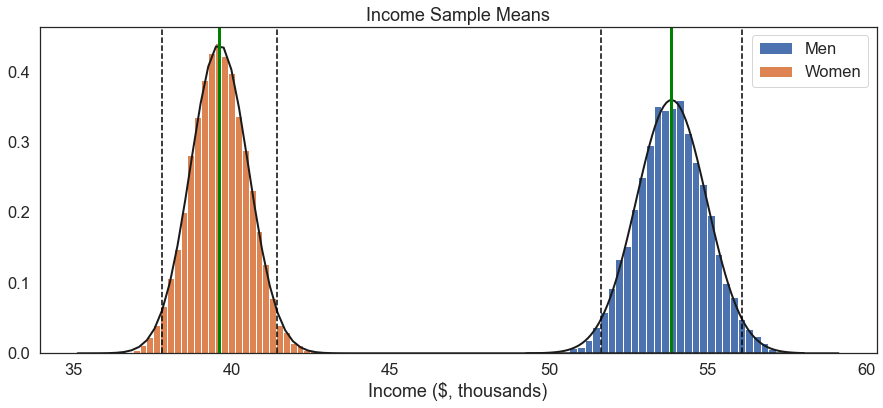
\includegraphics{notebooks/W04. Natural Language Processing_files/figure-pdf/cell-28-output-1.png}

}

\end{figure}

\begin{verbatim}
<AxesSubplot:xlabel='Samples', ylabel='Counts'>
\end{verbatim}

Now that we've produced counts for all words which conform to our list
of tags, we can quickly see how frequently common words appear; because
we have tokenized by sentence, we have to do this with a slightly
different mechanism - run through the words of interest and see how many
occurrences appear in the Frequency Distribution object, fd. Again,
we're sneaking in a FOR loop to run through these.

\begin{Shaded}
\begin{Highlighting}[]
\ControlFlowTok{for}\NormalTok{ word }\KeywordTok{in}\NormalTok{ [}\StringTok{\textquotesingle{}space\textquotesingle{}}\NormalTok{, }\StringTok{\textquotesingle{}nameless\textquotesingle{}}\NormalTok{, }\StringTok{\textquotesingle{}mad\textquotesingle{}}\NormalTok{, }\StringTok{\textquotesingle{}dread\textquotesingle{}}\NormalTok{, }\StringTok{\textquotesingle{}fear\textquotesingle{}}\NormalTok{, }\StringTok{\textquotesingle{}cthulhu\textquotesingle{}}\NormalTok{, }\StringTok{\textquotesingle{}necronomicon\textquotesingle{}}\NormalTok{, }\StringTok{\textquotesingle{}caring\textquotesingle{}}\NormalTok{]:}
    \BuiltInTok{print}\NormalTok{(word, fd[word])}
\end{Highlighting}
\end{Shaded}

\begin{verbatim}
space 279
nameless 174
mad 101
dread 49
fear 282
cthulhu 40
necronomicon 54
caring 0
\end{verbatim}

So far, we've completely avoided the use of pandas - but we can put this
data into a pandas dataframe very easily, and use the built-in graphing
methods to change the style of our graph.

We feed in fd.keys() - the words - and fd.values(), the wordcount.

\begin{Shaded}
\begin{Highlighting}[]
\CommentTok{\#Convert to list so subscriptable}
\BuiltInTok{list}\NormalTok{(fd.keys())[}\DecValTok{1}\NormalTok{:}\DecValTok{10}\NormalTok{]}
\end{Highlighting}
\end{Shaded}

\begin{verbatim}
['city', 'valley', 'moon', 'afar', 'sands', 'parts', 'corpse', 'grave', 'fear']
\end{verbatim}

\begin{Shaded}
\begin{Highlighting}[]
\CommentTok{\#Convert to list so subscriptable}
\BuiltInTok{list}\NormalTok{(fd.values())[}\DecValTok{1}\NormalTok{:}\DecValTok{10}\NormalTok{]}
\end{Highlighting}
\end{Shaded}

\begin{verbatim}
[456, 116, 276, 27, 17, 108, 36, 80, 282]
\end{verbatim}

\begin{Shaded}
\begin{Highlighting}[]
\ImportTok{import}\NormalTok{ pandas }\ImportTok{as}\NormalTok{ pd}

\CommentTok{\#Convert to list for use in creating dataframe}
\NormalTok{df }\OperatorTok{=}\NormalTok{ pd.DataFrame(\{}\StringTok{\textquotesingle{}items\textquotesingle{}}\NormalTok{: }\BuiltInTok{list}\NormalTok{(fd.keys()), }\StringTok{\textquotesingle{}counts\textquotesingle{}}\NormalTok{: }\BuiltInTok{list}\NormalTok{(fd.values())\})}
\NormalTok{df.head()}
\end{Highlighting}
\end{Shaded}

\begin{verbatim}
/Users/ollieballinger/.pyenv/versions/3.9.5/lib/python3.9/site-packages/pandas/compat/__init__.py:97: UserWarning: Could not import the lzma module. Your installed Python is incomplete. Attempting to use lzma compression will result in a RuntimeError.
  warnings.warn(msg)
\end{verbatim}

\begin{longtable}[]{@{}lll@{}}
\toprule()
& items & counts \\
\midrule()
\endhead
0 & nameless & 174 \\
1 & city & 456 \\
2 & valley & 116 \\
3 & moon & 276 \\
4 & afar & 27 \\
\bottomrule()
\end{longtable}

Let's now arrange them in order of appearance - the most common at the
top.

\begin{Shaded}
\begin{Highlighting}[]
\NormalTok{df }\OperatorTok{=}\NormalTok{ df.sort\_values(by}\OperatorTok{=}\StringTok{\textquotesingle{}counts\textquotesingle{}}\NormalTok{,ascending}\OperatorTok{=}\VariableTok{False}\NormalTok{)}
\NormalTok{df.head()}
\end{Highlighting}
\end{Shaded}

\begin{longtable}[]{@{}lll@{}}
\toprule()
& items & counts \\
\midrule()
\endhead
137 & time & 960 \\
18 & man & 884 \\
192 & things & 875 \\
38 & night & 725 \\
215 & thing & 667 \\
\bottomrule()
\end{longtable}

We now have a DataFrame with certain word tags sorted by decreasing
frequency. Let's plot this in a bar graph; we will use df{[}1:50{]} to
select the most common 50 words.

\begin{Shaded}
\begin{Highlighting}[]
\ImportTok{import}\NormalTok{ matplotlib.pyplot }\ImportTok{as}\NormalTok{ plt}
\end{Highlighting}
\end{Shaded}

\begin{Shaded}
\begin{Highlighting}[]
\NormalTok{plt.style.use(}\StringTok{\textquotesingle{}ggplot\textquotesingle{}}\NormalTok{)}
\NormalTok{df[}\DecValTok{1}\NormalTok{:}\DecValTok{50}\NormalTok{].plot(kind}\OperatorTok{=}\StringTok{\textquotesingle{}bar\textquotesingle{}}\NormalTok{, x}\OperatorTok{=}\StringTok{\textquotesingle{}items\textquotesingle{}}\NormalTok{, y}\OperatorTok{=}\StringTok{\textquotesingle{}counts\textquotesingle{}}\NormalTok{, legend}\OperatorTok{=}\VariableTok{False}\NormalTok{)}
\NormalTok{plt.xlabel(}\StringTok{\textquotesingle{}Word\textquotesingle{}}\NormalTok{)}
\NormalTok{plt.ylabel(}\StringTok{\textquotesingle{}Word Count\textquotesingle{}}\NormalTok{)}
\NormalTok{plt.title(}\StringTok{\textquotesingle{}Word counts for H.P. Lovecraft}\CharTok{\textbackslash{}\textquotesingle{}}\StringTok{s }\CharTok{\textbackslash{}"}\StringTok{The Nameless City}\CharTok{\textbackslash{}"}\StringTok{\textquotesingle{}}\NormalTok{)}
\NormalTok{plt.axhline(df[}\StringTok{\textquotesingle{}counts\textquotesingle{}}\NormalTok{].mean(), color}\OperatorTok{=}\StringTok{\textquotesingle{}\#2222ff\textquotesingle{}}\NormalTok{)}
\end{Highlighting}
\end{Shaded}

\begin{verbatim}
<matplotlib.lines.Line2D at 0x1888076a0>
\end{verbatim}

\begin{figure}[H]

{\centering 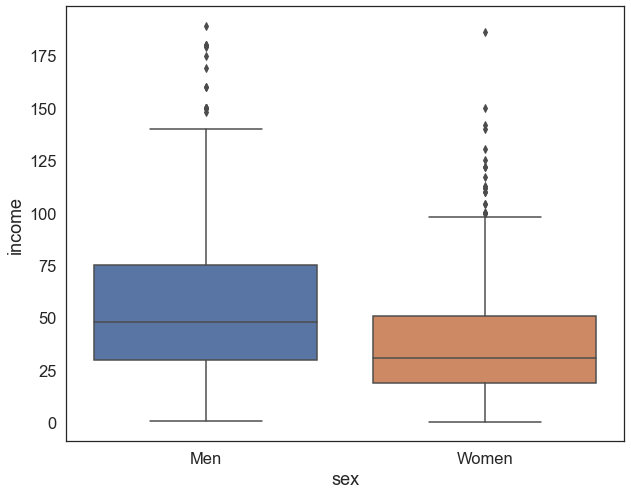
\includegraphics{notebooks/W04. Natural Language Processing_files/figure-pdf/cell-35-output-2.png}

}

\end{figure}

\hypertarget{exercise-11}{%
\section{Exercise}\label{exercise-11}}

What is the percentage of words that appear exactly once in the entire
text? (Hint : FreqDist objects have a method called `hapaxes')

\hypertarget{exercise-12}{%
\section{Exercise}\label{exercise-12}}

The words of our ex Prime Minister, David Cameron:

\begin{verbatim}
1. Select one of Cameron's speeches.
2. Sentence and word tokenize it.
3. POS tag it.
4. Create noun and adjective histograms of the 20 most frequent words.
(notice that there are several POS for each.)
5. Create dispersion plots for these nouns and adjectives. 
6. What is the percentage of words that are adjectives in the speech?
\end{verbatim}

\begin{Shaded}
\begin{Highlighting}[]
\CommentTok{\# read a raw text from a remote location. }
\NormalTok{speech }\OperatorTok{=}\NormalTok{ requests.get(}\StringTok{\textquotesingle{}https://s3.eu{-}west{-}2.amazonaws.com/qm2/wk7/speeches/cameron{-}leaders{-}speech{-}2006a.txt\textquotesingle{}}\NormalTok{).text}
\end{Highlighting}
\end{Shaded}

\hypertarget{speeches}{%
\subsection{Speeches}\label{speeches}}

https://s3.eu-west-2.amazonaws.com/qm2/wk7/speeches/cameron-election-victory-speech-2010.txt\\
https://s3.eu-west-2.amazonaws.com/qm2/wk7/speeches/cameron-leaders-speech-2006a.txt\\
https://s3.eu-west-2.amazonaws.com/qm2/wk7/speeches/cameron-leaders-speech-2006b.txt\\
https://s3.eu-west-2.amazonaws.com/qm2/wk7/speeches/cameron-leaders-speech-2007.txt\\
https://s3.eu-west-2.amazonaws.com/qm2/wk7/speeches/cameron-leaders-speech-2008.txt\\
https://s3.eu-west-2.amazonaws.com/qm2/wk7/speeches/cameron-leaders-speech-2013.txt\\
https://s3.eu-west-2.amazonaws.com/qm2/wk7/speeches/cameron-leaders-speech-2012.txt\\
https://s3.eu-west-2.amazonaws.com/qm2/wk7/speeches/cameron-leaders-speech-2011.txt\\
https://s3.eu-west-2.amazonaws.com/qm2/wk7/speeches/cameron-leaders-speech-2010.txt\\
https://s3.eu-west-2.amazonaws.com/qm2/wk7/speeches/cameron-leaders-speech-2009.txt

\begin{Shaded}
\begin{Highlighting}[]
\NormalTok{speech}
\end{Highlighting}
\end{Shaded}

\begin{verbatim}
'It\x92s a huge honour to be standing before you as leader of the Conservative Party.\r\n\r\n \r\n\r\nAnd first of all I want to thank you for the support you\x92ve given me in the past ten months.\r\n\r\n \r\n\r\nIt\x92s been a time of great change.\r\n\r\n \r\n\r\nI\x92m already on my second leader of the Liberal Democrats.\r\n\r\n \r\n\r\nBefore long I\x92ll be on to my second Labour Prime Minister.\r\n\r\n \r\n\r\nSoon I\x92ll be the longest-serving leader of a major British political party.\r\n\r\n \r\n\r\nI wanted this job for a very simple reason.\r\n\r\n \r\n\r\nI love this country.\r\n\r\n \r\n\r\nI have great ambitions for our future.\r\n\r\n \r\n\r\nAnd I want the Party I love\x85\r\n\r\n \r\n\r\n\x85to serve the country I love\x85\r\n\r\n \r\n\r\n\x85in helping Britain be the best that it can.\r\n\r\n \r\n\r\nWe need to change in order to have that chance.\r\n\r\n \r\n\r\nYou cannot shape the future if you\x92re stuck in the past.\r\n\r\n \r\n\r\nYou knew that.\r\n\r\n \r\n\r\nAnd that\x92s why you voted for change.\r\n\r\n \r\n\r\nI believe we can all be proud of what we\x92ve achieved these past ten months.\r\n\r\n \r\n\r\nPeople looking at us with new interest.\r\n\r\n \r\n\r\n25,000 new members.\r\n\r\n \r\n\r\nAnd in our first electoral test, in the local elections, we won forty per cent of the vote.\r\n\r\n \r\n\r\nLet\x92s hear it for our fantastic local councillors who worked so hard and won so well.\r\n\r\n \r\n\r\nTony Blair says it\x92s all style and no substance.\r\n\r\n \r\n\r\nIn fact he wrote me a letter about it.\r\n\r\n \r\n\r\nDear Kettle\x85\r\n\r\n \r\n\r\nYou\x92re black.\r\n\r\n \r\n\r\nSigned, Pot.\r\n\r\n \r\n\r\nWhat a nerve that man has got.\r\n\r\n \r\n\r\nIn the whole of the last year, there is only one substantial thing that the Labour Party has achieved for our country.\r\n\r\n \r\n\r\nTheir education reforms.\r\n\r\n \r\n\r\nRight now, across the country, trust schools are being prepared with greater freedoms to teach children the way teachers and parents want.\r\n\r\n \r\n\r\nThe only reason \x96 the only reason - that\x92s happening is because the Conservative Party did the right thing and took the legislation through the House of Commons.\r\n\r\n \r\n\r\nI\x92m proud of that \x96 proud of us, for putting the future of our children before party politics.\r\n\r\n \r\n\r\nAnother sign of our changing fortunes is the impressive array of speakers who have come to join us at our conference this year.\r\n\r\n \r\n\r\nSENATOR McCAIN\r\n\r\n \r\n\r\nAnd I\x92d like to pay a special tribute to one in particular.\r\n\r\n \r\n\r\nHe\x92s a man who knows about leadership.\r\n\r\n \r\n\r\nHe\x92s endured hardship that\x92s unimaginable to many of us here.\r\n\r\n \r\n\r\nAnd he\x92s fought battles for principles that we all admire.\r\n\r\n \r\n\r\nWho knows what the future may hold?\r\n\r\n \r\n\r\nBut John, I for one would be proud to see you \x96 a great American and a great friend to Britain - as leader of the free world.\r\n\r\n \r\n\r\nCOLLEAGUES\r\n\r\n \r\n\r\nI\x92d also like to pay tribute to my colleagues who have spoken already today.\r\n\r\n \r\n\r\nA year ago, David Davis and I were rivals.\r\n\r\n \r\n\r\nToday we\x92re partners.\r\n\r\n \r\n\r\nHe has given me the most fantastic support over these past ten months.\r\n\r\n \r\n\r\nIdeas, energy, advice.\r\n\r\n \r\n\r\nHe has not only helped bring this Party together\x85\r\n\r\n \r\n\r\n\x85he has helped take our Party in the right direction, and I want to thank him for all he\x92s done.\r\n\r\n \r\n\r\nAnd I\x92m proud to work with another man who is a brave politician, a wise counsellor and a great Conservative.\r\n\r\n \r\n\r\nA man who would be a Foreign Secretary that this country could be truly proud of: William Hague.\r\n\r\n \r\n\r\nThen there\x92s Francis.\r\n\r\n \r\n\r\nI know Francis likes to pretend that everything is doom and gloom.\r\n\r\n \r\n\r\nHe\x92s always talking about the mountain we have to climb.\r\n\r\n \r\n\r\nHe\x92s so gloomy, he makes Gordon Brown look like a ray of sunshine.\r\n\r\n \r\n\r\nBut Francis, you\x92re doing a great job.\r\n\r\n \r\n\r\nLABOUR SPLITS AND BACKSTABBING\r\n\r\n \r\n\r\nOf course Francis has long told us to avoid the point-scoring and name-calling that can give politics such a bad name.\r\n\r\n \r\n\r\nHe\x92s right.\r\n\r\n \r\n\r\nBut we didn\x92t bargain on the Labour Party.\r\n\r\n \r\n\r\nFirst Gordon said he could never trust Tony again, then Tony called Gordon a blackmailer.\r\n\r\n \r\n\r\nCharles said Gordon was stupid, then John popped up and said no, Tony was stupid.\r\n\r\n \r\n\r\nCharles called Gordon a deluded control freak.\r\n\r\n \r\n\r\nAnd a member of the Cabinet said \x93it would be an absolute effing disaster\x94 if Gordon got to No.10.\r\n\r\n \r\n\r\nThat was just the husbands.\r\n\r\n \r\n\r\nWhen I look at these Labour ministers I ask myself how much time they\x92re worrying about their own jobs\x85\r\n\r\n \r\n\r\n\x85and how much time they\x92re worrying about NHS, about crime, about our troops in Iraq and Afghanistan.\r\n\r\n \r\n\r\nYou only have to ask the question to know what the answer is.\r\n\r\n \r\n\r\nAnd there are months more of it still to come.\r\n\r\n \r\n\r\nMonths of infighting, instability, indecision, jockeying for position\x85\r\n\r\n \r\n\r\nThey said it would be a \x93stable and orderly transition.\x94\r\n\r\n \r\n\r\nYeah, right.\r\n\r\n \r\n\r\nLike they said \x9324 hours to save the NHS\x94, \x93education education education.\x94\r\n\r\n \r\n\r\nThese are the things they should be fighting for, but they\x92re too busy fighting each other.\r\n\r\n \r\n\r\nOUR RESPONSIBILITY\r\n\r\n \r\n\r\nSo we have a great responsibility.\r\n\r\n \r\n\r\nTo set out a clear, united and credible alternative.\r\n\r\n \r\n\r\nWith some elections, you just know the result before a single vote has been cast.\r\n\r\n \r\n\r\nWe were never going to win in 1997.\r\n\r\n \r\n\r\nPeople wanted change.\r\n\r\n \r\n\r\nI remember it well.\r\n\r\n \r\n\r\nI fought Stafford.\r\n\r\n \r\n\r\nAnd Stafford fought back.\r\n\r\n \r\n\r\nLabour were never going to win in 1983 when they offered Michael Foot as Prime Minister.\r\n\r\n \r\n\r\nOther elections are wide open.\r\n\r\n \r\n\r\nAnd the next election will be one of those.\r\n\r\n \r\n\r\nBut we will not win, nor deserve to win, without a clear purpose and a proper plan.\r\n\r\n \r\n\r\nWe must learn from Labour\x92s big mistake.\r\n\r\n \r\n\r\nWhen Tony Blair won his first election, he had only one clear purpose: to win a second term.\r\n\r\n \r\n\r\nEven now he says that the only legacy \x96 the only legacy - that really matters to him is Labour winning a fourth term.\r\n\r\n \r\n\r\nBack in 1997, he had no proper plan.\r\n\r\n \r\n\r\nNo real understanding of how to make change happen.\r\n\r\n \r\n\r\nHe had good intentions.\r\n\r\n \r\n\r\nBut he hadn\x92t worked out how to deliver them.\r\n\r\n \r\n\r\nSo New Labour went round and round in circles.\r\n\r\n \r\n\r\nThey abolished grant maintained schools - and now they\x92re trying to recreate them.\r\n\r\n \r\n\r\nThey reversed our NHS reforms - and now they\x92re trying to bring them back.\r\n\r\n \r\n\r\nRoad building \x96 cancelled, then reinstated.\r\n\r\n \r\n\r\nThey wasted time, wasted money, wasted the country\x92s goodwill.\r\n\r\n \r\n\r\nOnly now, after nine years, does Tony Blair seem clear about his purpose.\r\n\r\n \r\n\r\nWell I\x92m sorry Mr Blair.\r\n\r\n \r\n\r\nThat\x92s nine years too late.\r\n\r\n \r\n\r\nTHIS WEEK\r\n\r\n \r\n\r\nWe won\x92t make the same mistake.\r\n\r\n \r\n\r\nOn Wednesday, the last day of our conference, I want to talk in detail about the important issues we face as a nation \x96 and what our response will be.\r\n\r\n \r\n\r\nBut today, on this first day of our conference, I\x92d like to set the scene for our discussions this week.\r\n\r\n \r\n\r\nI want to explain how we will arrive at the next election knowing exactly what we want to do, and how we\x92re going to do it.\r\n\r\n \r\n\r\nMy argument is based on a simple analogy.\r\n\r\n \r\n\r\nGetting ready for the responsibility of government is like building a house together.\r\n\r\n \r\n\r\nThink of it in three stages.\r\n\r\n \r\n\r\nFirst you prepare the ground.\r\n\r\n \r\n\r\nThen you lay the foundations.\r\n\r\n \r\n\r\nAnd then, finally, brick by brick, you build your house.\r\n\r\n \r\n\r\nPREPARING THE GROUND\r\n\r\n \r\n\r\nThese last ten months, we have been preparing the ground.\r\n\r\n \r\n\r\nOur Party\x92s history tells us the ground on which political success is built.\r\n\r\n \r\n\r\nIt is the centre ground.\r\n\r\n \r\n\r\nNot the bog of political compromise.\r\n\r\n \r\n\r\nNot the ideological wilderness, out on the fringes of debate.\r\n\r\n \r\n\r\nBut the solid ground where people are.\r\n\r\n \r\n\r\nThe centre ground is where you find the concerns, the hopes and the dreams of most people and families in this country.\r\n\r\n \r\n\r\nIn 1979, they wanted a government to tame the unions, rescue our economy and restore Britain\x92s pride.\r\n\r\n \r\n\r\nMargaret Thatcher offered precisely that alternative.\r\n\r\n \r\n\r\nAnd this Party can forever take pride in her magnificent achievements.\r\n\r\n \r\n\r\nToday, people want different things.\r\n\r\n \r\n\r\nThe priorities are different.\r\n\r\n \r\n\r\nSafer streets.\r\n\r\n \r\n\r\nSchools that teach.\r\n\r\n \r\n\r\nA better quality of life.\r\n\r\n \r\n\r\nBetter treatment for carers.\r\n\r\n \r\n\r\nThat\x92s what people are talking about today.\r\n\r\n \r\n\r\nBut for too long, we were having a different conversation.\r\n\r\n \r\n\r\nInstead of talking about the things that most people care about, we talked about what we cared about most.\r\n\r\n \r\n\r\nWhile parents worried about childcare, getting the kids to school, balancing work and family life - we were banging on about Europe.\r\n\r\n \r\n\r\nAs they worried about standards in thousands of secondary schools, we obsessed about a handful more grammar schools.\r\n\r\n \r\n\r\nAs rising expectations demanded a better NHS for everyone, we put our faith in opt-outs for a few.\r\n\r\n \r\n\r\nWhile people wanted, more than anything, stability and low mortgage rates, the first thing we talked about was tax cuts.\r\n\r\n \r\n\r\nFor years, this country wanted \x96 desperately needed - a sensible centre-right party to sort things out in a sensible way.\r\n\r\n \r\n\r\nWell, that\x92s what we are today.\r\n\r\n \r\n\r\nIn these past ten months we have moved back to the ground on which this Party\x92s success has always been built.\r\n\r\n \r\n\r\nThe centre ground of British politics.\r\n\r\n \r\n\r\nAnd that is where we will stay.\r\n\r\n \r\n\r\nLAYING THE FOUNDATIONS \x96 SOCIAL RESPONSIBILITY\r\n\r\n \r\n\r\nBut preparing the ground is just the first stage.\r\n\r\n \r\n\r\nNow we must show what we will build there.\r\n\r\n \r\n\r\nA strong government needs strong foundations.\r\n\r\n \r\n\r\nAnd I want us to lay those foundations this week.\r\n\r\n \r\n\r\nThat\x92s not about individual policies.\r\n\r\n \r\n\r\nIt is about a vision of the Britain we want to see.\r\n\r\n \r\n\r\nA Britain where we do not just ask what government can do.\r\n\r\n \r\n\r\nWe ask what people can do, what society can do.\r\n\r\n \r\n\r\nA Britain where we stop thinking you can pass laws to make people good.\r\n\r\n \r\n\r\nAnd start realising that we are all in this together.\r\n\r\n \r\n\r\nSocial responsibility \x96 that is the essence of liberal Conservatism.\r\n\r\n \r\n\r\nThat is the idea I want us to explain this week.\r\n\r\n \r\n\r\nThat is what we stand for.\r\n\r\n \r\n\r\nThat is what we\x92re fighting for.\r\n\r\n \r\n\r\nThat is the Britain we want to build.\r\n\r\n \r\n\r\nTake fighting crime.\r\n\r\n \r\n\r\nIt is not just a state responsibility.\r\n\r\n \r\n\r\nIt is a social responsibility.\r\n\r\n \r\n\r\nLet\x92s not pretend that all we need is tough talk and tough laws to bring safety to our streets.\r\n\r\n \r\n\r\nOf course the state must play its part.\r\n\r\n \r\n\r\nThat\x92s why we\x92re developing a programme of radical police reform.\r\n\r\n \r\n\r\nThat\x92s why we want to build more prisons and reform the ones we\x92ve got, so they help reduce re-offending instead of encouraging it.\r\n\r\n \r\n\r\nAnd that\x92s why we\x92ll invest in drug rehabilitation, so we help addicts get clean and stay clean, instead of living a life of crime to feed their habit.\r\n\r\n \r\n\r\nBut that is not the end of the story.\r\n\r\n \r\n\r\nIt is just the start.\r\n\r\n \r\n\r\nWe need parents to bring up their children with the right values.\r\n\r\n \r\n\r\nWe need schools to be places of discipline and order.\r\n\r\n \r\n\r\nWe need to stand up for civilised values in public places.\r\n\r\n \r\n\r\nWe need to design crime out of the housing estates of the future.\r\n\r\n \r\n\r\nWe\x92ve got to stop selling alcohol to children.\r\n\r\n \r\n\r\nWe need the music industry to understand that profiting from violent and homophobic words and images is morally wrong and socially unacceptable.\r\n\r\n \r\n\r\nBut more than this, we need people, families, communities, businesses to step up to the plate and understand that it\x92s not just about stopping the bad things\x85\r\n\r\n \r\n\r\n\x85it\x92s about actively doing the good things.\r\n\r\n \r\n\r\nNot waiting for the state to do it all, but taking responsibility, making a difference, saying loudly and proudly: this is my country, this is my community: I will play my part.\r\n\r\n \r\n\r\nThat is social responsibility.\r\n\r\n \r\n\r\nThat is our idea.\r\n\r\n \r\n\r\nSo I want us to be the champions of a new spirit of social responsibility in this land.\r\n\r\n \r\n\r\nA new spirit of social responsibility that will succeed for Britain where Labour\x92s outdated state responsibility has failed.\r\n\r\n \r\n\r\nLABOUR\x92S APPROACH\r\n\r\n \r\n\r\nThink of any issue - not just crime - and then think of Labour\x92s response.\r\n\r\n \r\n\r\nThis Government\x92s way of doing things \x96 the old way of doing things - is so familiar, and so depressing.\r\n\r\n \r\n\r\nMinisters hold a summit.\r\n\r\n \r\n\r\nThey announce an eye-catching initiative.\r\n\r\n \r\n\r\nA five-year plan.\r\n\r\n \r\n\r\nGordon Brown generously finds the money for it.\r\n\r\n \r\n\r\nThe money gets a headline, but no-one knows what to do with it.\r\n\r\n \r\n\r\nSo they create a unit in the Cabinet Office.\r\n\r\n \r\n\r\nA task force is set up.\r\n\r\n \r\n\r\nRegional co-ordinators are appointed.\r\n\r\n \r\n\r\nGordon Brown sets them targets \x96 after all, it is his money.\r\n\r\n \r\n\r\nPilot schemes are launched.\r\n\r\n \r\n\r\nThe pilot schemes are rolled out across the country.\r\n\r\n \r\n\r\nThey are evaluated.\r\n\r\n \r\n\r\nThen revised, re-organised and re-launched.\r\n\r\n \r\n\r\nAnd then finally, once the reality dawns that the only people to benefit are the lawyers, accountants and consultants of Labour\x92s quango army\x85\r\n\r\n \r\n\r\n\x85with a pathetic whimper \x96 but no hint of an apology \x96 the whole thing is just abandoned.\r\n\r\n \r\n\r\nWe\x92ve seen too much of this in the past nine years.\r\n\r\n \r\n\r\nHeadline after headline but absolutely no follow-through.\r\n\r\n \r\n\r\nIt is a story of ignorance, incompetence, arrogance.\r\n\r\n \r\n\r\nA story of wasted billions - and disappointed millions.\r\n\r\n \r\n\r\nSomewhere out there, there is a place where Blair and Brown will never go.\r\n\r\n \r\n\r\nIt\x92s dark.\r\n\r\n \r\n\r\nIt\x92s depressing.\r\n\r\n \r\n\r\nIt\x92s haunted by the failures of nine years of centralisation, gimmick and spin.\r\n\r\n \r\n\r\nIt is the graveyard of initiatives, where you\x92ll find the e-University that died a death,\r\n\r\n \r\n\r\nthe drugs czar that came and went\x85\r\n\r\n \r\n\r\n\x85the Individual Learning Accounts that collapsed in fraud and waste, the tax credits that were paid and reclaimed\x85\r\n\r\n \r\n\r\n\x85the Connexions service that flopped, the Strategic Health Authorities that were dropped\x85\r\n\r\n \r\n\r\n\x85the marching of yobs to the hole in the wall; the night courts that never happened at all.\r\n\r\n \r\n\r\nAnd still they keep coming, those hubristic monuments to big government, the living dead that walk the well-trodden path from Downing Street and the Treasury to New Labour\x92s graveyard of initiatives.\r\n\r\n \r\n\r\nThe NHS computer: delayed, disorganised, a £20 billion shambles.\r\n\r\n \r\n\r\nForced police mergers: the direct opposite of the community policing we need.\r\n\r\n \r\n\r\nAnd then the perfect example.\r\n\r\n \r\n\r\nID cards.\r\n\r\n \r\n\r\nWhen a half-way competent government would be protecting our security by controlling our borders\x85\r\n\r\n \r\n\r\n\x85these Labour ministers are pressing ahead with their vast white elephant, their plastic poll tax, twenty Millennium Domes rolled into one giant catastrophe in the making.\r\n\r\n \r\n\r\nThey\x92ve given up trying to find a good reason for it.\r\n\r\n \r\n\r\nLast week Tony Blair said that ID cards would help control immigration, when new immigrants won\x92t even have them.\r\n\r\n \r\n\r\nDoes he even know what\x92s going on in his Government?\r\n\r\n \r\n\r\nID cards are wrong, they\x92re a waste of money, and we will abolish them.\r\n\r\n \r\n\r\nThese last nine years have been the story of a Government which instinctively believes, whatever it says, that everything is the state\x92s responsibility.\r\n\r\n \r\n\r\nWe believe in social responsibility.\r\n\r\n \r\n\r\nBecause there is such a thing as society, it\x92s just not the same thing as the state.\r\n\r\n \r\n\r\nTHE BRITAIN WE WANT TO SEE\r\n\r\n \r\n\r\nSo let us define this week the kind of Britain we want to see.\r\n\r\n \r\n\r\nAnd let us show how our idea \x96 social responsibility\x85\r\n\r\n \r\n\r\n\x85not Labour\x92s idea \x96 state responsibility\x85\r\n\r\n \r\n\r\n\x85is the right response to the challenges Britain faces.\r\n\r\n \r\n\r\nGLOBALISATION, WELL-BEING, THE ENVIRONMENT\r\n\r\n \r\n\r\nWe know that in the age of globalisation, in the face of fast-moving economic change, people want their government to provide security.\r\n\r\n \r\n\r\nWe know that the end of the traditional 9 to 5 job can make life tough for families, and people look to their government for answers.\r\n\r\n \r\n\r\nAnd we know that in the race against time to tackle climate change and protect the environment, people expect their government to show leadership.\r\n\r\n \r\n\r\nOn all these challenges, Labour\x92s first response is to regulate business, hoping to offer protection.\r\n\r\n \r\n\r\nIt may sound attractive.\r\n\r\n \r\n\r\nBut there are unintended consequences.\r\n\r\n \r\n\r\nWell-intentioned regulation can make us less secure in the age of globalisation.\r\n\r\n \r\n\r\nLess able to provide the jobs, wealth and opportunity on which well-being depends.\r\n\r\n \r\n\r\nIt can undermine the competitiveness of our companies, so it\x92s harder for them to invest in the new, green technologies of the future.\r\n\r\n \r\n\r\nSo our response, based on our philosophy of social responsibility, is to say to business:\r\n\r\n \r\n\r\nYes you should look after your workers, yes you should look after your community, yes you should look after our environment.\r\n\r\n \r\n\r\nAnd we must stand up to big business when it\x92s in the interests of Britain and the wider world.\r\n\r\n \r\n\r\nSo next week our MEPs will vote to strengthen proposals to make companies replace dangerous chemicals with safe ones.\r\n\r\n \r\n\r\nBut where Labour are casual about increasing regulation, we will be careful.\r\n\r\n \r\n\r\nWe will ask:\r\n\r\n \r\n\r\nAre we making it easier to start a business?\r\n\r\n \r\n\r\nEasier to employ someone?\r\n\r\n \r\n\r\nIs the overall burden of regulation going down?\r\n\r\n \r\n\r\nWill the regulation that\x92s being put forward lead to real changes in behaviour, or just time-wasting and box-ticking?\r\n\r\n \r\n\r\nIf only we had a government that was asking these questions today.\r\n\r\n \r\n\r\nWe want companies to create their own solutions to social and environmental challenges, because those are the solutions most likely to last.\r\n\r\n \r\n\r\nSo in a Conservative Britain, corporate responsibility will provide the best long-term answer to economic insecurity, well-being in the workplace, and environmental care.\r\n\r\n \r\n\r\nIt is the same approach when you look at the other great challenges we face.\r\n\r\n \r\n\r\nPUBLIC SERVICES\r\n\r\n \r\n\r\nWe know that in an age of amazing technological advance, instant information exchange, and empowered consumers who don\x92t have the deference of previous generations\x85\r\n\r\n \r\n\r\n\x85people expect more from our health service and our schools.\r\n\r\n \r\n\r\nAnd government has to respond to that.\r\n\r\n \r\n\r\nLabour\x92s response is the culture of targets, directives and central control, aimed at raising standards in our public services.\r\n\r\n \r\n\r\nThey mean well.\r\n\r\n \r\n\r\nBut the unintended consequence is to make these services less responsive to the people who use them, dashing expectations not meeting them.\r\n\r\n \r\n\r\nSo our response, based on our philosophy of social responsibility, is to say to our nurses, doctors, teachers:\r\n\r\n \r\n\r\nYes you should meet higher standards, yes you should give your patients and your pupils more.\r\n\r\n \r\n\r\nBut we\x92re not going to tell you how to do it.\r\n\r\n \r\n\r\nYou are professionals.\r\n\r\n \r\n\r\nWe trust in your vocation\r\n\r\n \r\n\r\nSo in a Conservative Britain, professional responsibility will provide the answer to rising expectations in the NHS and schools.\r\n\r\n \r\n\r\nPOVERTY AND REGENERATION\r\n\r\n \r\n\r\nAnd just as people will no longer accept second best in public services, we know that in their communities they are fed up with squalor and poverty and crime\x85\r\n\r\n \r\n\r\n\x85and they look to their leaders to sort things out.\r\n\r\n \r\n\r\nLabour\x92s response has been a massive expansion of central government into local communities.\r\n\r\n \r\n\r\nThe centralised Neighbourhood Renewal Unit, the insensitive Pathfinder programme, prescriptive top-down schemes for regeneration.\r\n\r\n \r\n\r\nYou can see why Labour have done it.\r\n\r\n \r\n\r\nBut the unintended consequence is to stifle the very spirit of community self-improvement that they are responding to.\r\n\r\n \r\n\r\nOur response, based on our philosophy of social responsibility, is to trust local leaders, not undermine them.\r\n\r\n \r\n\r\nSo we will hand power and control to local councils and local people who have the solutions to poverty, to crime, to urban decay in their hands.\r\n\r\n \r\n\r\nWe trust in your knowledge and commitment.\r\n\r\n \r\n\r\nSo in a Conservative Britain, civic responsibility will provide the answer to improving the quality of life in the communities left behind.\r\n\r\n \r\n\r\nCHILDREN\r\n\r\n \r\n\r\nAnd then perhaps the greatest challenge of all.\r\n\r\n \r\n\r\nThe challenge of bringing up children in a world that often seems fraught with risk and danger.\r\n\r\n \r\n\r\nThere is nothing that matters more to me than the safety and happiness of my family.\r\n\r\n \r\n\r\nOf course it\x92s right that government should be on parents\x92 side.\r\n\r\n \r\n\r\nBut Labour take it way too far.\r\n\r\n \r\n\r\nA national database of every child.\r\n\r\n \r\n\r\nMaking childcare a state monopoly.\r\n\r\n \r\n\r\nSlapping ASBOs on children who haven\x92t even been born.\r\n\r\n \r\n\r\nLabour\x92s intentions may be good.\r\n\r\n \r\n\r\nBut the unintended consequence is to create a culture of irresponsibility.\r\n\r\n \r\n\r\nThey may have abandoned Clause 4 and the nationalisation of industry.\r\n\r\n \r\n\r\nBut they are replacing it with the nationalisation of everyday life.\r\n\r\n \r\n\r\nThe state can never be everywhere, policing the interactions of our daily lives - and it shouldn\x92t try.\r\n\r\n \r\n\r\nReal change will take years of patient hard work, and we will test every policy by asking: does it enhance parental responsibility?\r\n\r\n \r\n\r\nWe need to understand that cultural change is worth any number of government initiatives.\r\n\r\n \r\n\r\nWho has done more to improve school food, Jamie Oliver, or the Department of Education?\r\n\r\n \r\n\r\nPut another way, we need more of Supernanny, less of the nanny state.\r\n\r\n \r\n\r\nSo in a Conservative Britain, personal responsibility will provide the best answer to the risks and dangers of the modern world.\r\n\r\n \r\n\r\nPersonal responsibility.\r\n\r\n \r\n\r\nProfessional responsibility.\r\n\r\n \r\n\r\nCorporate responsibility.\r\n\r\n \r\n\r\nCivic responsibility.\r\n\r\n \r\n\r\nThese are the four pillars of our social responsibility.\r\n\r\n \r\n\r\nThat is the Britain we want to build.\r\n\r\n \r\n\r\nA Britain that is more green.\r\n\r\n \r\n\r\nMore family-friendly.\r\n\r\n \r\n\r\nMore local control over the things that matter.\r\n\r\n \r\n\r\nLess arrogant about politicians\x92 ability to do it all on their own.\r\n\r\n \r\n\r\nBut more optimistic about what we can achieve if we all work together.\r\n\r\n \r\n\r\nWe want an opportunity society, not an overpowering state.\r\n\r\n \r\n\r\nBUILDING OUR HOUSE\r\n\r\n \r\n\r\nThis week, in our debates, we will lay the foundations of the house we are building together.\r\n\r\n \r\n\r\nThe foundations must come first.\r\n\r\n \r\n\r\nHow superficial, how insubstantial it would be, for us to make up policies to meet the pressures of the moment.\r\n\r\n \r\n\r\nPolicy without principle is like a house without foundations.\r\n\r\n \r\n\r\nIt will not stand the test of time.\r\n\r\n \r\n\r\nThat is what our Policy Review is all about: getting it right for the long term.\r\n\r\n \r\n\r\nOPTIMISM ABOUT BRITAIN\x92S FUTURE\r\n\r\n \r\n\r\nIf we do this, we can help achieve so much for this country.\r\n\r\n \r\n\r\nIn a few years\x92 time, Britain could wake up to a bright new morning.\r\n\r\n \r\n\r\nWe have everything to be optimistic about.\r\n\r\n \r\n\r\nYou could not design a country with better natural advantages than we have.\r\n\r\n \r\n\r\nWe speak the language of the world.\r\n\r\n \r\n\r\nWe have links of history and culture with every continent on earth.\r\n\r\n \r\n\r\nWe have institutions \x96 our legal system, our armed forces, the BBC, our great universities \x96 which set the standard that all other countries measure themselves by.\r\n\r\n \r\n\r\nOur artists, writers and musicians inspire people the world over.\r\n\r\n \r\n\r\nWe are inventive, creative, irreverent and daring.\r\n\r\n \r\n\r\nIn this young century, these old advantages give us the edge we need.\r\n\r\n \r\n\r\nCONCLUSION\r\n\r\n \r\n\r\nWhat a prospect for a great Party \x96 to guide our nation at this time of opportunity.\r\n\r\n \r\n\r\nSo let us stick to the plan.\r\n\r\n \r\n\r\nLet us build - carefully, thoughtfully and patiently, a new house together.\r\n\r\n \r\n\r\nPreparing the ground as we move to the centre, meeting the priorities of the modern world.\r\n\r\n \r\n\r\nLaying the foundations with our idea - social responsibility.\r\n\r\n \r\n\r\nAnd building on those foundations with the right policies for our long-term future.\r\n\r\n \r\n\r\nThe nation\x92s hopes are in our hands.\r\n\r\n \r\n\r\nPeople\x92s hopes.\r\n\r\n \r\n\r\nYour hopes.\r\n\r\n \r\n\r\nMy hopes.\r\n\r\n \r\n\r\nIn eight days\x92 time I will be forty years old.\r\n\r\n \r\n\r\nI have so much to look forward to.\r\n\r\n \r\n\r\nMy young family.\r\n\r\n \r\n\r\nThey have so much to look forward to.\r\n\r\n \r\n\r\nThe world I want for them is the world I want for every family and every community.\r\n\r\n \r\n\r\nIf you want to know what I\x92m all about, I can explain it one word.\r\n\r\n \r\n\r\nThat word is optimism.\r\n\r\n \r\n\r\nI am optimistic about human nature.\r\n\r\n \r\n\r\nThat\x92s why I will trust people to do the right thing.\r\n\r\n \r\n\r\nLabour are pessimists.\r\n\r\n \r\n\r\nThey think that without their guidance, people will do the wrong thing.\r\n\r\n \r\n\r\nThat\x92s why they want to regulate and control.\r\n\r\n \r\n\r\nSo let us show clearly which side we are on.\r\n\r\n \r\n\r\nLet optimism beat pessimism.\r\n\r\n \r\n\r\nLet sunshine win the day.\r\n\r\n \r\n\r\nAnd let everyone know that the Conservative Party is ready.\r\n\r\n \r\n\r\nReady to serve.\r\n\r\n \r\n\r\nReady to fight.\r\n\r\n \r\n\r\nReady to win.'
\end{verbatim}

\bookmarksetup{startatroot}

\hypertarget{merging-and-joining}{%
\chapter{Merging and Joining}\label{merging-and-joining}}

\hypertarget{workshop-5-open-in-colab}{%
\section[\emph{Workshop 5} ]{\texorpdfstring{\emph{Workshop 5}
\href{https://colab.research.google.com/github/oballinger/QM2/blob/main/notebooks/W05.\%20Merging\%20and\%20Joining.ipynb}{\protect
\includegraphics{notebooks/../colab-badge.png}}}{Workshop 5 Open In Colab}}\label{workshop-5-open-in-colab}}

Sometimes, we will want to combine data from different sources about the
same subject - perhaps we want to compare the GDP in a country with life
expectancy, or the proportion of free schools meals with the level of
unemployment.

\hypertarget{aims-2}{%
\subsection{Aims}\label{aims-2}}

\begin{itemize}
\tightlist
\item
  Understand joins
\item
  Work with joining dataframes in Pandas
\item
  Create your own examples
\end{itemize}

\hypertarget{downloading-the-data-3}{%
\section{Downloading the Data}\label{downloading-the-data-3}}

Let's grab the data we will need this week from our course website and
save it into our data folder. If you've not already created a data
folder then do so using the following command.

Don't worry if it generates an error, that means you've already got a
data folder.

\begin{Shaded}
\begin{Highlighting}[]
\OperatorTok{!}\NormalTok{mkdir data}
\end{Highlighting}
\end{Shaded}

\begin{verbatim}
mkdir: data: File exists
\end{verbatim}

\begin{Shaded}
\begin{Highlighting}[]
\OperatorTok{!}\NormalTok{mkdir data}\OperatorTok{/}\NormalTok{wk3}
\OperatorTok{!}\NormalTok{curl https:}\OperatorTok{//}\NormalTok{s3.eu}\OperatorTok{{-}}\NormalTok{west}\OperatorTok{{-}}\FloatTok{2.}\ErrorTok{amazonaws}\NormalTok{.com}\OperatorTok{/}\NormalTok{qm2}\OperatorTok{/}\NormalTok{wk3}\OperatorTok{/}\NormalTok{UN\_Life\_all.csv }\OperatorTok{{-}}\NormalTok{o .}\OperatorTok{/}\NormalTok{data}\OperatorTok{/}\NormalTok{wk5}\OperatorTok{/}\NormalTok{UN\_Life\_all.csv}
\OperatorTok{!}\NormalTok{curl https:}\OperatorTok{//}\NormalTok{s3.eu}\OperatorTok{{-}}\NormalTok{west}\OperatorTok{{-}}\FloatTok{2.}\ErrorTok{amazonaws}\NormalTok{.com}\OperatorTok{/}\NormalTok{qm2}\OperatorTok{/}\NormalTok{wk3}\OperatorTok{/}\NormalTok{UN\_Cities\_1214\_country.csv }\OperatorTok{{-}}\NormalTok{o .}\OperatorTok{/}\NormalTok{data}\OperatorTok{/}\NormalTok{wk5}\OperatorTok{/}\NormalTok{UN\_Cities\_1214\_country.csv}
\OperatorTok{!}\NormalTok{curl https:}\OperatorTok{//}\NormalTok{s3.eu}\OperatorTok{{-}}\NormalTok{west}\OperatorTok{{-}}\FloatTok{2.}\ErrorTok{amazonaws}\NormalTok{.com}\OperatorTok{/}\NormalTok{qm2}\OperatorTok{/}\NormalTok{wk3}\OperatorTok{/}\NormalTok{UN\_Cities\_1214\_population.csv }\OperatorTok{{-}}\NormalTok{o .}\OperatorTok{/}\NormalTok{data}\OperatorTok{/}\NormalTok{wk5}\OperatorTok{/}\NormalTok{UN\_Cities\_1214\_population.csv}
\end{Highlighting}
\end{Shaded}

\begin{verbatim}
mkdir: data/wk3: File exists
  % Total    % Received % Xferd  Average Speed   Time    Time     Time  Current
                                 Dload  Upload   Total   Spent    Left  Speed
  0     0    0     0    0     0      0      0 --:--:-- --:--:-- --:--:--     0Warning: Failed to create the file ./data/wk5/UN_Life_all.csv: No such file or 
Warning: directory
  4  354k    4 15915    0     0  36914      0  0:00:09 --:--:--  0:00:09 37271
curl: (23) Failure writing output to destination
  % Total    % Received % Xferd  Average Speed   Time    Time     Time  Current
                                 Dload  Upload   Total   Spent    Left  Speed
  0     0    0     0    0     0      0      0 --:--:-- --:--:-- --:--:--     0Warning: Failed to create the file ./data/wk5/UN_Cities_1214_country.csv: No 
Warning: such file or directory
 52 31445   52 16384    0     0  32380      0 --:--:-- --:--:-- --:--:-- 32833
curl: (23) Failure writing output to destination
  % Total    % Received % Xferd  Average Speed   Time    Time     Time  Current
                                 Dload  Upload   Total   Spent    Left  Speed
  0     0    0     0    0     0      0      0 --:--:-- --:--:-- --:--:--     0Warning: Failed to create the file ./data/wk5/UN_Cities_1214_population.csv: 
Warning: No such file or directory
  0  373k    0  1580    0     0   3234      0  0:01:58 --:--:--  0:01:58  3284
curl: (23) Failure writing output to destination
\end{verbatim}

\hypertarget{joining-instructions}{%
\section{Joining Instructions}\label{joining-instructions}}

Joins are the combination of different datasets, and are common in
relational databases as a way of performing queries. There are lots of
examples of why and when we might want to do this, but most start with
two tables of data. We're going to start with some data we've generated.

I'm going to go back and work with fake data for a while, because it's
clean and small and we can see what's going on - when we work with real
data, we have to take great care that the data is clean, the indices
match, and so on.

\begin{Shaded}
\begin{Highlighting}[]
\ImportTok{import}\NormalTok{ matplotlib.pyplot }\ImportTok{as}\NormalTok{ plt}
\ImportTok{import}\NormalTok{ pandas }\ImportTok{as}\NormalTok{ pd}
\ImportTok{import}\NormalTok{ numpy }\ImportTok{as}\NormalTok{ np}
\ImportTok{import}\NormalTok{ random}
\OperatorTok{\%}\NormalTok{matplotlib inline}
\end{Highlighting}
\end{Shaded}

Let's create dataframes which represent fictitious values associated
with people. Let's assume our data is anonymised because we're ethical
researchers and don't want information about real people leaking out.

\begin{Shaded}
\begin{Highlighting}[]
\NormalTok{people1 }\OperatorTok{=}\NormalTok{ pd.DataFrame(}\DecValTok{5}\OperatorTok{+}\NormalTok{np.random.randn(}\DecValTok{5}\NormalTok{, }\DecValTok{5}\NormalTok{))}
\NormalTok{people1.columns }\OperatorTok{=}\NormalTok{ [}\StringTok{\textquotesingle{}units of alcohol drunk\textquotesingle{}}\NormalTok{,}\StringTok{\textquotesingle{}cigarettes smoked\textquotesingle{}}\NormalTok{,}\StringTok{\textquotesingle{}sleep per night\textquotesingle{}}\NormalTok{,}\StringTok{\textquotesingle{}height\textquotesingle{}}\NormalTok{,}\StringTok{\textquotesingle{}BMI\textquotesingle{}}\NormalTok{]}
\end{Highlighting}
\end{Shaded}

\begin{Shaded}
\begin{Highlighting}[]
\NormalTok{people1}
\end{Highlighting}
\end{Shaded}

\begin{longtable}[]{@{}llllll@{}}
\toprule()
& units of alcohol drunk & cigarettes smoked & sleep per night & height
& BMI \\
\midrule()
\endhead
0 & 6.053520 & 5.767268 & 4.521370 & 4.315644 & 6.513931 \\
1 & 3.845497 & 5.102046 & 4.397347 & 7.332429 & 3.944509 \\
2 & 5.433980 & 5.129674 & 2.899948 & 5.641938 & 5.147669 \\
3 & 4.461049 & 6.897319 & 6.241158 & 3.693360 & 5.240822 \\
4 & 6.095539 & 4.239457 & 3.986249 & 4.525927 & 4.374219 \\
\bottomrule()
\end{longtable}

\begin{Shaded}
\begin{Highlighting}[]
\NormalTok{people2 }\OperatorTok{=}\NormalTok{ pd.DataFrame(}\DecValTok{5}\OperatorTok{+}\NormalTok{np.random.randn(}\DecValTok{3}\NormalTok{, }\DecValTok{5}\NormalTok{))}
\NormalTok{people2.columns }\OperatorTok{=}\NormalTok{ [}\StringTok{\textquotesingle{}units of alcohol drunk\textquotesingle{}}\NormalTok{,}\StringTok{\textquotesingle{}cigarettes smoked\textquotesingle{}}\NormalTok{,}\StringTok{\textquotesingle{}sleep per night\textquotesingle{}}\NormalTok{,}\StringTok{\textquotesingle{}height\textquotesingle{}}\NormalTok{,}\StringTok{\textquotesingle{}BMI\textquotesingle{}}\NormalTok{]}
\end{Highlighting}
\end{Shaded}

\begin{Shaded}
\begin{Highlighting}[]
\NormalTok{people2}
\end{Highlighting}
\end{Shaded}

\begin{longtable}[]{@{}llllll@{}}
\toprule()
& units of alcohol drunk & cigarettes smoked & sleep per night & height
& BMI \\
\midrule()
\endhead
0 & 5.060422 & 5.479779 & 5.134008 & 4.705505 & 6.048511 \\
1 & 5.996277 & 5.845720 & 2.615113 & 5.479796 & 4.905734 \\
2 & 4.979671 & 5.011475 & 6.751763 & 6.605953 & 4.257274 \\
\bottomrule()
\end{longtable}

\bookmarksetup{startatroot}

\hypertarget{adding-new-observations}{%
\chapter{Adding new observations}\label{adding-new-observations}}

It looks as if we have some data about people (although we've just made
it up), and a set of common measurements. It would be nice to have all
of this in one place, so let's \emph{merge} them into one dataframe.
We'll use the \emph{concat} command, which is short for
\emph{concatenate}, or ``chain together''.

\begin{Shaded}
\begin{Highlighting}[]
\NormalTok{people3 }\OperatorTok{=}\NormalTok{ pd.concat([people1,people2])}
\end{Highlighting}
\end{Shaded}

\begin{Shaded}
\begin{Highlighting}[]
\NormalTok{people3}
\end{Highlighting}
\end{Shaded}

\begin{longtable}[]{@{}llllll@{}}
\toprule()
& units of alcohol drunk & cigarettes smoked & sleep per night & height
& BMI \\
\midrule()
\endhead
0 & 6.053520 & 5.767268 & 4.521370 & 4.315644 & 6.513931 \\
1 & 3.845497 & 5.102046 & 4.397347 & 7.332429 & 3.944509 \\
2 & 5.433980 & 5.129674 & 2.899948 & 5.641938 & 5.147669 \\
3 & 4.461049 & 6.897319 & 6.241158 & 3.693360 & 5.240822 \\
4 & 6.095539 & 4.239457 & 3.986249 & 4.525927 & 4.374219 \\
0 & 5.060422 & 5.479779 & 5.134008 & 4.705505 & 6.048511 \\
1 & 5.996277 & 5.845720 & 2.615113 & 5.479796 & 4.905734 \\
2 & 4.979671 & 5.011475 & 6.751763 & 6.605953 & 4.257274 \\
\bottomrule()
\end{longtable}

\hypertarget{what-is-the-problem-above}{%
\subsection{What is the problem
above?}\label{what-is-the-problem-above}}

\begin{Shaded}
\begin{Highlighting}[]
\NormalTok{people4 }\OperatorTok{=}\NormalTok{ pd.concat([people1,people2], ignore\_index}\OperatorTok{=}\VariableTok{True}\NormalTok{)}
\end{Highlighting}
\end{Shaded}

\begin{Shaded}
\begin{Highlighting}[]
\NormalTok{people4}
\end{Highlighting}
\end{Shaded}

\begin{longtable}[]{@{}llllll@{}}
\toprule()
& units of alcohol drunk & cigarettes smoked & sleep per night & height
& BMI \\
\midrule()
\endhead
0 & 6.053520 & 5.767268 & 4.521370 & 4.315644 & 6.513931 \\
1 & 3.845497 & 5.102046 & 4.397347 & 7.332429 & 3.944509 \\
2 & 5.433980 & 5.129674 & 2.899948 & 5.641938 & 5.147669 \\
3 & 4.461049 & 6.897319 & 6.241158 & 3.693360 & 5.240822 \\
4 & 6.095539 & 4.239457 & 3.986249 & 4.525927 & 4.374219 \\
5 & 5.060422 & 5.479779 & 5.134008 & 4.705505 & 6.048511 \\
6 & 5.996277 & 5.845720 & 2.615113 & 5.479796 & 4.905734 \\
7 & 4.979671 & 5.011475 & 6.751763 & 6.605953 & 4.257274 \\
\bottomrule()
\end{longtable}

\texttt{ignore\_index} is very useful when we want a new DataFrame which
only contains data from other DataFrames, but unrelated otherwise.

\hypertarget{data-with-a-unique-index-adding-new-observations}{%
\section{Data with a unique index: adding new
observations}\label{data-with-a-unique-index-adding-new-observations}}

Let's now examine data where the elements of study are not anonymous.
Let's consider that we have some city data. If we have city names (or
equivalent) in the index column, simply concatenating them would be
fine, because the names would not repeat in the way the index has above.

\begin{Shaded}
\begin{Highlighting}[]
\NormalTok{df1 }\OperatorTok{=}\NormalTok{ pd.DataFrame(}\DecValTok{5}\OperatorTok{+}\NormalTok{np.random.randn(}\DecValTok{5}\NormalTok{, }\DecValTok{5}\NormalTok{))}
\NormalTok{df1.columns }\OperatorTok{=}\NormalTok{ [}\StringTok{\textquotesingle{}area\textquotesingle{}}\NormalTok{,}\StringTok{\textquotesingle{}population\textquotesingle{}}\NormalTok{,}\StringTok{\textquotesingle{}mean temperature\textquotesingle{}}\NormalTok{,}\StringTok{\textquotesingle{}elevation\textquotesingle{}}\NormalTok{,}\StringTok{\textquotesingle{}annual rainfall\textquotesingle{}}\NormalTok{]}
\NormalTok{df1.index }\OperatorTok{=}\NormalTok{ [}\StringTok{\textquotesingle{}London\textquotesingle{}}\NormalTok{, }\StringTok{\textquotesingle{}Paris\textquotesingle{}}\NormalTok{, }\StringTok{\textquotesingle{}Beijing\textquotesingle{}}\NormalTok{, }\StringTok{\textquotesingle{}Medellin\textquotesingle{}}\NormalTok{, }\StringTok{\textquotesingle{}Port Elizabeth\textquotesingle{}}\NormalTok{]}
\end{Highlighting}
\end{Shaded}

\begin{Shaded}
\begin{Highlighting}[]
\NormalTok{df1}
\end{Highlighting}
\end{Shaded}

\begin{longtable}[]{@{}llllll@{}}
\toprule()
& area & population & mean temperature & elevation & annual rainfall \\
\midrule()
\endhead
London & 5.077016 & 3.344452 & 7.000945 & 5.854193 & 4.457887 \\
Paris & 3.631221 & 5.323007 & 4.579731 & 3.598146 & 6.832792 \\
Beijing & 4.598318 & 4.187428 & 5.287178 & 5.074045 & 3.491496 \\
Medellin & 6.213580 & 4.411090 & 5.798357 & 5.241598 & 6.739662 \\
Port Elizabeth & 5.416446 & 4.351028 & 6.595819 & 5.297740 & 3.935567 \\
\bottomrule()
\end{longtable}

\begin{Shaded}
\begin{Highlighting}[]
\NormalTok{df2 }\OperatorTok{=}\NormalTok{ pd.DataFrame(}\DecValTok{5}\OperatorTok{+}\NormalTok{np.random.randn(}\DecValTok{3}\NormalTok{, }\DecValTok{5}\NormalTok{))}
\NormalTok{df2.columns }\OperatorTok{=}\NormalTok{ [}\StringTok{\textquotesingle{}area\textquotesingle{}}\NormalTok{,}\StringTok{\textquotesingle{}population\textquotesingle{}}\NormalTok{,}\StringTok{\textquotesingle{}mean temperature\textquotesingle{}}\NormalTok{,}\StringTok{\textquotesingle{}elevation\textquotesingle{}}\NormalTok{,}\StringTok{\textquotesingle{}annual rainfall\textquotesingle{}}\NormalTok{]}
\NormalTok{df2.index }\OperatorTok{=}\NormalTok{ [}\StringTok{\textquotesingle{}Mumbai\textquotesingle{}}\NormalTok{, }\StringTok{\textquotesingle{}Sydney\textquotesingle{}}\NormalTok{, }\StringTok{\textquotesingle{}Boston\textquotesingle{}}\NormalTok{]}
\end{Highlighting}
\end{Shaded}

\begin{Shaded}
\begin{Highlighting}[]
\NormalTok{df2}
\end{Highlighting}
\end{Shaded}

\begin{longtable}[]{@{}llllll@{}}
\toprule()
& area & population & mean temperature & elevation & annual rainfall \\
\midrule()
\endhead
Mumbai & 5.403218 & 5.646440 & 5.259170 & 6.065506 & 5.657623 \\
Sydney & 6.807486 & 4.278180 & 4.786912 & 4.375484 & 4.119702 \\
Boston & 4.651726 & 5.190903 & 5.123513 & 6.541282 & 4.807702 \\
\bottomrule()
\end{longtable}

\begin{Shaded}
\begin{Highlighting}[]
\NormalTok{df3 }\OperatorTok{=}\NormalTok{ pd.concat([df1,df2])}
\end{Highlighting}
\end{Shaded}

\begin{Shaded}
\begin{Highlighting}[]
\NormalTok{df3}
\end{Highlighting}
\end{Shaded}

\begin{longtable}[]{@{}llllll@{}}
\toprule()
& area & population & mean temperature & elevation & annual rainfall \\
\midrule()
\endhead
London & 5.077016 & 3.344452 & 7.000945 & 5.854193 & 4.457887 \\
Paris & 3.631221 & 5.323007 & 4.579731 & 3.598146 & 6.832792 \\
Beijing & 4.598318 & 4.187428 & 5.287178 & 5.074045 & 3.491496 \\
Medellin & 6.213580 & 4.411090 & 5.798357 & 5.241598 & 6.739662 \\
Port Elizabeth & 5.416446 & 4.351028 & 6.595819 & 5.297740 & 3.935567 \\
Mumbai & 5.403218 & 5.646440 & 5.259170 & 6.065506 & 5.657623 \\
Sydney & 6.807486 & 4.278180 & 4.786912 & 4.375484 & 4.119702 \\
Boston & 4.651726 & 5.190903 & 5.123513 & 6.541282 & 4.807702 \\
\bottomrule()
\end{longtable}

\hypertarget{exercise-concat-continued}{%
\section{Exercise: Concat continued}\label{exercise-concat-continued}}

Repeat the above for fictitious values for New York, Tokyo, Manila and
Budapest - concatenate into a new dataframe ``df''.

\hypertarget{combining-on-attributes}{%
\section{Combining on Attributes}\label{combining-on-attributes}}

What if we're looking at the same locations but different attributes?
Consider the same df1

\begin{Shaded}
\begin{Highlighting}[]
\NormalTok{df1 }\OperatorTok{=}\NormalTok{ pd.DataFrame(}\DecValTok{5}\OperatorTok{+}\NormalTok{np.random.randn(}\DecValTok{5}\NormalTok{, }\DecValTok{5}\NormalTok{))}
\NormalTok{df1.columns }\OperatorTok{=}\NormalTok{ [}\StringTok{\textquotesingle{}area\textquotesingle{}}\NormalTok{,}\StringTok{\textquotesingle{}population\textquotesingle{}}\NormalTok{,}\StringTok{\textquotesingle{}mean temperature\textquotesingle{}}\NormalTok{,}\StringTok{\textquotesingle{}elevation\textquotesingle{}}\NormalTok{,}\StringTok{\textquotesingle{}annual rainfall\textquotesingle{}}\NormalTok{]}
\NormalTok{df1.index }\OperatorTok{=}\NormalTok{ [}\StringTok{\textquotesingle{}London\textquotesingle{}}\NormalTok{, }\StringTok{\textquotesingle{}Paris\textquotesingle{}}\NormalTok{, }\StringTok{\textquotesingle{}Beijing\textquotesingle{}}\NormalTok{, }\StringTok{\textquotesingle{}Medellin\textquotesingle{}}\NormalTok{, }\StringTok{\textquotesingle{}Port Elizabeth\textquotesingle{}}\NormalTok{]}
\end{Highlighting}
\end{Shaded}

\begin{Shaded}
\begin{Highlighting}[]
\NormalTok{df1}
\end{Highlighting}
\end{Shaded}

\begin{longtable}[]{@{}llllll@{}}
\toprule()
& area & population & mean temperature & elevation & annual rainfall \\
\midrule()
\endhead
London & 5.348823 & 5.486505 & 5.105354 & 3.680852 & 4.487838 \\
Paris & 5.670247 & 5.812321 & 4.076454 & 6.701972 & 3.781139 \\
Beijing & 5.707170 & 6.253187 & 3.172944 & 5.131476 & 4.993762 \\
Medellin & 4.852207 & 3.773460 & 5.652641 & 5.607786 & 4.481264 \\
Port Elizabeth & 4.320782 & 5.476499 & 5.685651 & 5.537774 & 4.264993 \\
\bottomrule()
\end{longtable}

But a new dataframe df4, which details the same locations, but has
different information about them:

\begin{Shaded}
\begin{Highlighting}[]
\NormalTok{df4 }\OperatorTok{=}\NormalTok{ pd.DataFrame(}\DecValTok{5}\OperatorTok{+}\NormalTok{np.random.randn(}\DecValTok{5}\NormalTok{, }\DecValTok{3}\NormalTok{))}
\NormalTok{df4.columns }\OperatorTok{=}\NormalTok{ [}\StringTok{\textquotesingle{}Mean House Price\textquotesingle{}}\NormalTok{, }\StringTok{\textquotesingle{}median income\textquotesingle{}}\NormalTok{,}\StringTok{\textquotesingle{}walkability score\textquotesingle{}}\NormalTok{]}
\NormalTok{df4.index }\OperatorTok{=}\NormalTok{ [}\StringTok{\textquotesingle{}London\textquotesingle{}}\NormalTok{, }\StringTok{\textquotesingle{}Paris\textquotesingle{}}\NormalTok{, }\StringTok{\textquotesingle{}Beijing\textquotesingle{}}\NormalTok{, }\StringTok{\textquotesingle{}Medellin\textquotesingle{}}\NormalTok{, }\StringTok{\textquotesingle{}Port Elizabeth\textquotesingle{}}\NormalTok{]}
\end{Highlighting}
\end{Shaded}

\begin{Shaded}
\begin{Highlighting}[]
\NormalTok{df4}
\end{Highlighting}
\end{Shaded}

\begin{longtable}[]{@{}llll@{}}
\toprule()
& Mean House Price & median income & walkability score \\
\midrule()
\endhead
London & 4.400513 & 3.878475 & 5.134940 \\
Paris & 4.221475 & 4.966409 & 3.641013 \\
Beijing & 5.131144 & 6.189124 & 5.357512 \\
Medellin & 5.250745 & 5.765428 & 4.313135 \\
Port Elizabeth & 3.748654 & 5.078490 & 4.935660 \\
\bottomrule()
\end{longtable}

We have to join ``on'' the index - meaning when merging the records,
python will look at the index column.

\begin{Shaded}
\begin{Highlighting}[]
\NormalTok{df\_joined }\OperatorTok{=}\NormalTok{ df1.merge(df4, left\_index}\OperatorTok{=}\VariableTok{True}\NormalTok{, right\_index}\OperatorTok{=}\VariableTok{True}\NormalTok{)}
\end{Highlighting}
\end{Shaded}

\begin{Shaded}
\begin{Highlighting}[]
\NormalTok{df\_joined}
\end{Highlighting}
\end{Shaded}

\begin{longtable}[]{@{}lllllllll@{}}
\toprule()
& area & population & mean temperature & elevation & annual rainfall &
Mean House Price & median income & walkability score \\
\midrule()
\endhead
London & 5.348823 & 5.486505 & 5.105354 & 3.680852 & 4.487838 & 4.400513
& 3.878475 & 5.134940 \\
Paris & 5.670247 & 5.812321 & 4.076454 & 6.701972 & 3.781139 & 4.221475
& 4.966409 & 3.641013 \\
Beijing & 5.707170 & 6.253187 & 3.172944 & 5.131476 & 4.993762 &
5.131144 & 6.189124 & 5.357512 \\
Medellin & 4.852207 & 3.773460 & 5.652641 & 5.607786 & 4.481264 &
5.250745 & 5.765428 & 4.313135 \\
Port Elizabeth & 4.320782 & 5.476499 & 5.685651 & 5.537774 & 4.264993 &
3.748654 & 5.078490 & 4.935660 \\
\bottomrule()
\end{longtable}

Note that this joins on the \emph{index}, not the row number - so if the
order of elements in df4 is different, it should still work.

\begin{Shaded}
\begin{Highlighting}[]
\NormalTok{df4 }\OperatorTok{=}\NormalTok{ pd.DataFrame(np.random.randn(}\DecValTok{5}\NormalTok{, }\DecValTok{3}\NormalTok{))}
\NormalTok{df4.columns }\OperatorTok{=}\NormalTok{ [}\StringTok{\textquotesingle{}Mean House Price\textquotesingle{}}\NormalTok{, }\StringTok{\textquotesingle{}median income\textquotesingle{}}\NormalTok{,}\StringTok{\textquotesingle{}walkability score\textquotesingle{}}\NormalTok{]}
\NormalTok{df4.index }\OperatorTok{=}\NormalTok{ [}\StringTok{\textquotesingle{}Paris\textquotesingle{}}\NormalTok{,}\StringTok{\textquotesingle{}Port Elizabeth\textquotesingle{}}\NormalTok{, }\StringTok{\textquotesingle{}Beijing\textquotesingle{}}\NormalTok{, }\StringTok{\textquotesingle{}Medellin\textquotesingle{}}\NormalTok{, }\StringTok{\textquotesingle{}London\textquotesingle{}}\NormalTok{]}
\end{Highlighting}
\end{Shaded}

\begin{Shaded}
\begin{Highlighting}[]
\NormalTok{df1}
\end{Highlighting}
\end{Shaded}

\begin{longtable}[]{@{}llllll@{}}
\toprule()
& area & population & mean temperature & elevation & annual rainfall \\
\midrule()
\endhead
London & 5.348823 & 5.486505 & 5.105354 & 3.680852 & 4.487838 \\
Paris & 5.670247 & 5.812321 & 4.076454 & 6.701972 & 3.781139 \\
Beijing & 5.707170 & 6.253187 & 3.172944 & 5.131476 & 4.993762 \\
Medellin & 4.852207 & 3.773460 & 5.652641 & 5.607786 & 4.481264 \\
Port Elizabeth & 4.320782 & 5.476499 & 5.685651 & 5.537774 & 4.264993 \\
\bottomrule()
\end{longtable}

\begin{Shaded}
\begin{Highlighting}[]
\NormalTok{df4}
\end{Highlighting}
\end{Shaded}

\begin{longtable}[]{@{}llll@{}}
\toprule()
& Mean House Price & median income & walkability score \\
\midrule()
\endhead
Paris & 0.191529 & 0.428600 & -1.627663 \\
Port Elizabeth & 1.002571 & -0.171798 & -0.780653 \\
Beijing & -2.158222 & 0.494159 & 0.825195 \\
Medellin & -0.147067 & 0.864457 & -0.790751 \\
London & 0.856815 & -0.571106 & 0.417661 \\
\bottomrule()
\end{longtable}

\begin{Shaded}
\begin{Highlighting}[]
\NormalTok{df\_joined }\OperatorTok{=}\NormalTok{ df1.merge(df4, left\_index}\OperatorTok{=}\VariableTok{True}\NormalTok{, right\_index}\OperatorTok{=}\VariableTok{True}\NormalTok{)}
\end{Highlighting}
\end{Shaded}

\begin{Shaded}
\begin{Highlighting}[]
\NormalTok{df\_joined}
\end{Highlighting}
\end{Shaded}

\begin{longtable}[]{@{}lllllllll@{}}
\toprule()
& area & population & mean temperature & elevation & annual rainfall &
Mean House Price & median income & walkability score \\
\midrule()
\endhead
London & 5.348823 & 5.486505 & 5.105354 & 3.680852 & 4.487838 & 0.856815
& -0.571106 & 0.417661 \\
Paris & 5.670247 & 5.812321 & 4.076454 & 6.701972 & 3.781139 & 0.191529
& 0.428600 & -1.627663 \\
Beijing & 5.707170 & 6.253187 & 3.172944 & 5.131476 & 4.993762 &
-2.158222 & 0.494159 & 0.825195 \\
Medellin & 4.852207 & 3.773460 & 5.652641 & 5.607786 & 4.481264 &
-0.147067 & 0.864457 & -0.790751 \\
Port Elizabeth & 4.320782 & 5.476499 & 5.685651 & 5.537774 & 4.264993 &
1.002571 & -0.171798 & -0.780653 \\
\bottomrule()
\end{longtable}

\hypertarget{merge-records}{%
\section{Merge Records}\label{merge-records}}

Consider now a case where we have data for some but not all cities; so
df1 stil has data for these 5 cities:

\begin{Shaded}
\begin{Highlighting}[]
\NormalTok{df1}
\end{Highlighting}
\end{Shaded}

\begin{longtable}[]{@{}llllll@{}}
\toprule()
& area & population & mean temperature & elevation & annual rainfall \\
\midrule()
\endhead
London & 5.348823 & 5.486505 & 5.105354 & 3.680852 & 4.487838 \\
Paris & 5.670247 & 5.812321 & 4.076454 & 6.701972 & 3.781139 \\
Beijing & 5.707170 & 6.253187 & 3.172944 & 5.131476 & 4.993762 \\
Medellin & 4.852207 & 3.773460 & 5.652641 & 5.607786 & 4.481264 \\
Port Elizabeth & 4.320782 & 5.476499 & 5.685651 & 5.537774 & 4.264993 \\
\bottomrule()
\end{longtable}

But our new table, df5, contains data for three cities:

\begin{Shaded}
\begin{Highlighting}[]
\NormalTok{df5 }\OperatorTok{=}\NormalTok{ pd.DataFrame(}\DecValTok{5}\OperatorTok{+}\NormalTok{np.random.randn(}\DecValTok{3}\NormalTok{, }\DecValTok{3}\NormalTok{))}
\NormalTok{df5.columns }\OperatorTok{=}\NormalTok{ [}\StringTok{\textquotesingle{}Mean House Price\textquotesingle{}}\NormalTok{, }\StringTok{\textquotesingle{}median income\textquotesingle{}}\NormalTok{,}\StringTok{\textquotesingle{}walkability score\textquotesingle{}}\NormalTok{]}
\NormalTok{df5.index }\OperatorTok{=}\NormalTok{ [}\StringTok{\textquotesingle{}London\textquotesingle{}}\NormalTok{, }\StringTok{\textquotesingle{}Paris\textquotesingle{}}\NormalTok{, }\StringTok{\textquotesingle{}Glasgow\textquotesingle{}}\NormalTok{]}
\end{Highlighting}
\end{Shaded}

\begin{Shaded}
\begin{Highlighting}[]
\NormalTok{df5}
\end{Highlighting}
\end{Shaded}

\begin{longtable}[]{@{}llll@{}}
\toprule()
& Mean House Price & median income & walkability score \\
\midrule()
\endhead
London & 6.115865 & 5.045850 & 4.932779 \\
Paris & 4.115616 & 5.671406 & 6.329527 \\
Glasgow & 5.830768 & 3.804848 & 4.211793 \\
\bottomrule()
\end{longtable}

\hypertarget{exercise-13}{%
\section{Exercise:}\label{exercise-13}}

How many cities appear in: - both dataframes - only df1 - only df5 -
neither df1 nor df5?

\hypertarget{way-back-venn}{%
\section{Way Back Venn}\label{way-back-venn}}

What is the mechanism for joining data where these mismatches exist?
Well, there are several, starting with the\ldots{}

\hypertarget{inner-join}{%
\section{Inner Join:}\label{inner-join}}

\begin{Shaded}
\begin{Highlighting}[]
\ImportTok{from}\NormalTok{ IPython.display }\ImportTok{import}\NormalTok{ Image}

\NormalTok{data\_path }\OperatorTok{=} \StringTok{"https://s3.eu{-}west{-}2.amazonaws.com/qm2/wk3/inner.png"}
\NormalTok{Image(data\_path)}
\end{Highlighting}
\end{Shaded}

\begin{figure}[H]

{\centering 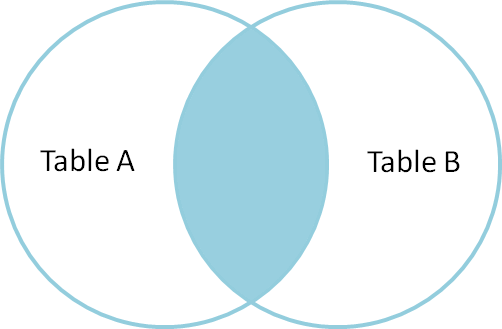
\includegraphics{notebooks/W05. Merging and Joining_files/figure-pdf/cell-33-output-1.png}

}

\end{figure}

(Image from
http://blog.codinghorror.com/a-visual-explanation-of-sql-joins/)

The inner join \emph{only} includes data whose index appears in both
tables. Let's see what that looks like:

\begin{Shaded}
\begin{Highlighting}[]
\NormalTok{df\_joined }\OperatorTok{=}\NormalTok{ df1.merge(df5, left\_index}\OperatorTok{=}\VariableTok{True}\NormalTok{, right\_index}\OperatorTok{=}\VariableTok{True}\NormalTok{)}
\end{Highlighting}
\end{Shaded}

\begin{Shaded}
\begin{Highlighting}[]
\NormalTok{df\_joined}
\end{Highlighting}
\end{Shaded}

\begin{longtable}[]{@{}lllllllll@{}}
\toprule()
& area & population & mean temperature & elevation & annual rainfall &
Mean House Price & median income & walkability score \\
\midrule()
\endhead
London & 5.348823 & 5.486505 & 5.105354 & 3.680852 & 4.487838 & 6.115865
& 5.045850 & 4.932779 \\
Paris & 5.670247 & 5.812321 & 4.076454 & 6.701972 & 3.781139 & 4.115616
& 5.671406 & 6.329527 \\
\bottomrule()
\end{longtable}

Here, we have a couple of arguments specifying the manner of the join -
we have specified that we are joining on the index of the left and right
dataset with the optional ``left\_index=True'' and
``right\_index=True''. Less obviously, the \textbf{left} dataset is df1
(because we're using \emph{df1.merge()} and the \textbf{right} dataset
is df5 (because it appears as an argument in merge(). There's no special
reason it shouldn't be the other way around, but for this function, it
is this way around and we need to remember that when we use it.

\hypertarget{inner-space}{%
\section{Inner Space}\label{inner-space}}

Although we haven't specified it, the merge() function has defaulted to
an inner join (like the diagram above). We can specify how the join is
calculated by changing the text in the optional argument ``how'':

\begin{Shaded}
\begin{Highlighting}[]
\NormalTok{df\_joined }\OperatorTok{=}\NormalTok{ df1.merge(df5, left\_index}\OperatorTok{=}\VariableTok{True}\NormalTok{, right\_index}\OperatorTok{=}\VariableTok{True}\NormalTok{, how}\OperatorTok{=}\StringTok{\textquotesingle{}inner\textquotesingle{}}\NormalTok{)}
\end{Highlighting}
\end{Shaded}

\begin{Shaded}
\begin{Highlighting}[]
\NormalTok{df\_joined}
\end{Highlighting}
\end{Shaded}

\begin{longtable}[]{@{}lllllllll@{}}
\toprule()
& area & population & mean temperature & elevation & annual rainfall &
Mean House Price & median income & walkability score \\
\midrule()
\endhead
London & 5.348823 & 5.486505 & 5.105354 & 3.680852 & 4.487838 & 6.115865
& 5.045850 & 4.932779 \\
Paris & 5.670247 & 5.812321 & 4.076454 & 6.701972 & 3.781139 & 4.115616
& 5.671406 & 6.329527 \\
\bottomrule()
\end{longtable}

\hypertarget{the-future-of-the-left}{%
\section{The Future of The Left}\label{the-future-of-the-left}}

The \emph{left} join includes \textbf{all} rows where the index appears
on the \textbf{left} hand side of the join, and \textbf{any} data which
\textbf{matches} it on the \textbf{right} hand side. If the index
appears on the left but not the right, it will include the data from the
left table, and have blanks for the columns on the right.

\begin{Shaded}
\begin{Highlighting}[]
\NormalTok{data\_path }\OperatorTok{=} \StringTok{"https://s3.eu{-}west{-}2.amazonaws.com/qm2/wk3/left.png"}
\NormalTok{Image(data\_path)}
\end{Highlighting}
\end{Shaded}

\begin{figure}[H]

{\centering 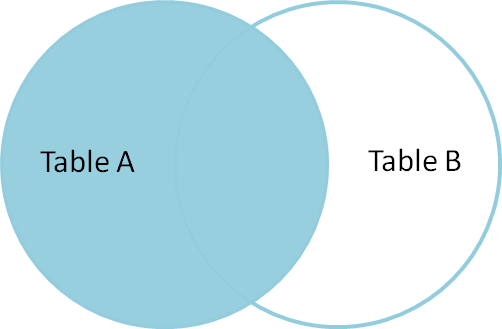
\includegraphics{notebooks/W05. Merging and Joining_files/figure-pdf/cell-38-output-1.png}

}

\end{figure}

What does \emph{this} look like? We will use the \emph{how=`left'}
optional argument to create a left join:

\begin{Shaded}
\begin{Highlighting}[]
\NormalTok{df\_joined }\OperatorTok{=}\NormalTok{ df1.merge(df5, left\_index}\OperatorTok{=}\VariableTok{True}\NormalTok{, right\_index}\OperatorTok{=}\VariableTok{True}\NormalTok{, how}\OperatorTok{=}\StringTok{\textquotesingle{}left\textquotesingle{}}\NormalTok{)}
\end{Highlighting}
\end{Shaded}

\begin{Shaded}
\begin{Highlighting}[]
\NormalTok{df\_joined}
\end{Highlighting}
\end{Shaded}

\begin{longtable}[]{@{}lllllllll@{}}
\toprule()
& area & population & mean temperature & elevation & annual rainfall &
Mean House Price & median income & walkability score \\
\midrule()
\endhead
London & 5.348823 & 5.486505 & 5.105354 & 3.680852 & 4.487838 & 6.115865
& 5.045850 & 4.932779 \\
Paris & 5.670247 & 5.812321 & 4.076454 & 6.701972 & 3.781139 & 4.115616
& 5.671406 & 6.329527 \\
Beijing & 5.707170 & 6.253187 & 3.172944 & 5.131476 & 4.993762 & NaN &
NaN & NaN \\
Medellin & 4.852207 & 3.773460 & 5.652641 & 5.607786 & 4.481264 & NaN &
NaN & NaN \\
Port Elizabeth & 4.320782 & 5.476499 & 5.685651 & 5.537774 & 4.264993 &
NaN & NaN & NaN \\
\bottomrule()
\end{longtable}

As we see, the missing data appears as \textbf{NaN} - Not a Number.

\hypertarget{exercise-14}{%
\section{Exercise:}\label{exercise-14}}

Carry out \emph{right} and \emph{outer} joins on the dataframes df1 and
df5 and explain how they're filtering and joining the data.

\hypertarget{i-am-the-one-and-only}{%
\section{I Am The One and Only}\label{i-am-the-one-and-only}}

So far, we've carried out joins on data which have a \emph{one-to-one}
relationship; data for cities or people. What if our data has a
\emph{one-to-many} correspondence?

\emph{Example:} We want to look at the quality of life in cities (a real
student project from 2014). We have a dataset listing city-level
characteristics for a number of cities in Europe, including the country
each city is in. We also have a dataset listing the GDP, life expectancy
and other indicators for a number of \emph{countries} in Europe. How do
we create a dataframe which, for each city, lists all of the
characteristics of a city and those of its parent country?

We'll be working now with data from the UN, covering information about
cities - real data this time. The UN has some great data, we've taken
some from here and processed it in various ways:

http://data.un.org/Data.aspx?d=POP\&f=tableCode\%3A240

Let's load up data on city population - this set contains data for
2012-2014 inclusive:

\begin{Shaded}
\begin{Highlighting}[]
\NormalTok{data\_path }\OperatorTok{=} \StringTok{"./data/wk3/UN\_Cities\_1214\_population.csv"}

\NormalTok{city\_pop }\OperatorTok{=}\NormalTok{ pd.read\_csv(data\_path, encoding}\OperatorTok{=}\StringTok{\textquotesingle{}latin1\textquotesingle{}}\NormalTok{)}
\end{Highlighting}
\end{Shaded}

\begin{Shaded}
\begin{Highlighting}[]
\NormalTok{city\_pop.head()}
\end{Highlighting}
\end{Shaded}

\begin{longtable}[]{@{}lllllllllll@{}}
\toprule()
& Year & Area & Sex & City & City type & Record Type & Reliability &
Source Year & Value & Value Footnotes \\
\midrule()
\endhead
0 & 2013 & Total & Both Sexes & MARIEHAMN & City proper & Estimate - de
jure & Final figure, complete & 2014 & 11370.0 & NaN \\
1 & 2013 & Total & Male & MARIEHAMN & City proper & Estimate - de jure &
Final figure, complete & 2014 & 5445.0 & NaN \\
2 & 2013 & Total & Female & MARIEHAMN & City proper & Estimate - de jure
& Final figure, complete & 2014 & 5925.0 & NaN \\
3 & 2012 & Total & Both Sexes & MARIEHAMN & City proper & Estimate - de
jure & Final figure, complete & 2013 & 11304.5 & NaN \\
4 & 2012 & Total & Male & MARIEHAMN & City proper & Estimate - de jure &
Final figure, complete & 2013 & 5408.0 & NaN \\
\bottomrule()
\end{longtable}

\hypertarget{exercise-15}{%
\section{Exercise}\label{exercise-15}}

There is a another datafile we downloaded called
\emph{UN\_Cities\_1214\_country.csv}. This is saved to
\emph{./data/wk3/UN\_Cities\_1214\_country.csv} - Load this into a
dataframe called \emph{city\_c} with the city name as the index and view
it; then, using \emph{merge} on city name with city\_pop to create a new
dataframe called \emph{cities}.

\textbf{Hints:} You'll notice that the index \textbf{won't} be the
column you want to merge on in the city\_pop data. What column
\emph{should} you merge on in city\_pop? Which column should you merge
on in city\_c?

The syntax for merging on a \textbf{column} (which is not the index) is
to pass the column name to the optional `left\_on=' or `right\_on='
arguments. And we don't use right\_index=True (or left\_index=True),
depending on which we're using.

So for example: \textbf{df1.merge(df2, left\_on=`Name',
right\_index=True)} would join df1 (on the left) to df2 (on the right),
using the column `Name' on the left (df1) and the index column (whatever
that is) on the right (df2).

\hypertarget{a-footnote-about-footnotes}{%
\section{A footnote about footnotes}\label{a-footnote-about-footnotes}}

Just a quick note - if you look at the primary UN data, you'll see
footnotes which will confuse the hell out of Pandas. I've taken the
footnotes out, but you can use .tail() to see whether there's any junk
in the trunk, and remove it via a text editor.

\hypertarget{clean-data}{%
\section{Clean data}\label{clean-data}}

We need to simplify this data a bit in the following ways:

\begin{enumerate}
\def\labelenumi{\arabic{enumi}.}
\tightlist
\item
  I'm going to focus on one year (2012)
\item
  I'm going to just look at ``Both Sexes'' (not focus on one gender)
\item
  I'm going to get rid of a column of data (the `Value Footnotes'
  column) using the \emph{drop()} method.
\end{enumerate}

\begin{Shaded}
\begin{Highlighting}[]
\NormalTok{cities }\OperatorTok{=}\NormalTok{ cities[cities[}\StringTok{\textquotesingle{}Sex\textquotesingle{}}\NormalTok{]}\OperatorTok{==}\StringTok{\textquotesingle{}Both Sexes\textquotesingle{}}\NormalTok{]}
\NormalTok{cities }\OperatorTok{=}\NormalTok{ cities[cities[}\StringTok{\textquotesingle{}Year\textquotesingle{}}\NormalTok{]}\OperatorTok{==}\DecValTok{2012}\NormalTok{]}
\NormalTok{cities.drop(}\StringTok{\textquotesingle{}Value Footnotes\textquotesingle{}}\NormalTok{, axis}\OperatorTok{=}\DecValTok{1}\NormalTok{, inplace}\OperatorTok{=}\VariableTok{True}\NormalTok{)}
\end{Highlighting}
\end{Shaded}

\begin{verbatim}
NameError: name 'cities' is not defined
\end{verbatim}

\begin{Shaded}
\begin{Highlighting}[]
\NormalTok{cities.head()}
\end{Highlighting}
\end{Shaded}

\hypertarget{extension-in-my-place}{%
\section{Extension: In My Place}\label{extension-in-my-place}}

The command I used to get rid of that column is \emph{cities.drop(`Value
Footnotes', axis=1, inplace=True)}. The syntax is not so complex - the
first argument, \emph{`Value Footnotes'}, is just the name of the
column; the second argument, \emph{axis=1}, tells Pandas to look for a
column to remove (instead of a row which has \emph{axis=0}); the third
and final argument, \emph{inplace=True}, is a command that tells Pandas
to edit \emph{inplace}, i.e.~to edit the dataframe (\emph{cities})
directly. When \emph{inplace} is False (the default), this command does
not directly edit cities, but instead provide an output. So the syntax
for that would be

new\_cities = cities.drop(`Value Footnotes', axis=1)

and new\_cities would be a version of \emph{cities} without the
offending column. This is usually the safer option.

\hypertarget{life-oh-life}{%
\section{Life, Oh Life}\label{life-oh-life}}

The UN also has useful data by country, so let's try and work with some
of that and join it up with our city data. Let's work with Life
Expectancy Data:

http://data.un.org/Data.aspx?d=WDI\&f=Indicator\_Code\%3ASP.DYN.LE00.IN

\begin{Shaded}
\begin{Highlighting}[]
\NormalTok{data\_path }\OperatorTok{=} \StringTok{"./data/wk3/UN\_Life\_all.csv"}
\NormalTok{life }\OperatorTok{=}\NormalTok{ pd.read\_csv(data\_path, index\_col}\OperatorTok{=}\DecValTok{0}\NormalTok{)}
\end{Highlighting}
\end{Shaded}

\begin{Shaded}
\begin{Highlighting}[]
\NormalTok{life.head()}
\end{Highlighting}
\end{Shaded}

\hypertarget{exercise-16}{%
\section{Exercise:}\label{exercise-16}}

In a new cell, clean up the above dataframe by

\begin{itemize}
\tightlist
\item
  removing the ``Value Footnotes'' Column
\item
  use only the most recent data (2012)
\end{itemize}

Let's make it a little clearer what ``Value'' refers to, by renaming the
column. This is one way to do that:

\begin{Shaded}
\begin{Highlighting}[]
\NormalTok{life.rename(columns}\OperatorTok{=}\NormalTok{\{}\StringTok{\textquotesingle{}Value\textquotesingle{}}\NormalTok{:}\StringTok{\textquotesingle{}Life Expectancy\textquotesingle{}}\NormalTok{\}, inplace}\OperatorTok{=}\VariableTok{True}\NormalTok{)}
\end{Highlighting}
\end{Shaded}

\begin{Shaded}
\begin{Highlighting}[]
\NormalTok{life.head()}
\end{Highlighting}
\end{Shaded}

\bookmarksetup{startatroot}

\hypertarget{exercise-17}{%
\chapter{Exercise}\label{exercise-17}}

Now, merge this data with the cities data to show life expectancy for
each city (based on the country it is in), and show the first 5 rows.

How much data was ``missing'' in the merge?

Relabel the City Population column so it's clear what it represents.

\textbf{Extension:} Plot population against life expectancy. Use plot's
\emph{optional arguments} to specify the x column, y column, and that
kind=`scatter'.

\textbf{Don't forget to include a title and axis labels!}

How does London fit in this trend? What are the problems with doing
this?

\hypertarget{recap-joins}{%
\section{Recap: Joins}\label{recap-joins}}

Pandas has \textbf{four} join methods:

\begin{verbatim}
- Left Join: use **only** keys from **left** DataFrame. SQL: [left outer join](http://goo.gl/JICveI)
- Right Join: use **only** keys from **right** DataFrame. SQL: [right outer join](http://goo.gl/TrrHjQ)
- Outer Join: use union of **keys from both** DataFrames. SQL: [full outer join](http://goo.gl/bVRqO8)
- Inner Join: use **intersection of keys** from both DataFrames. SQL: [inner join](http://goo.gl/Cf1MF8)
\end{verbatim}

\bookmarksetup{startatroot}

\hypertarget{group-presentations}{%
\chapter{Group Presentations}\label{group-presentations}}

\bookmarksetup{startatroot}

\hypertarget{distributions-and-basic-statistics}{%
\chapter{Distributions and Basic
Statistics}\label{distributions-and-basic-statistics}}

\hypertarget{workshop-7-open-in-colab}{%
\section[\emph{Workshop 7} ]{\texorpdfstring{\emph{Workshop 7}
\href{https://colab.research.google.com/github/oballinger/QM2/blob/main/notebooks/W07.\%20Distributions\%20and\%20Basic\%20Statistics.ipynb}{\protect
\includegraphics{notebooks/../colab-badge.png}}}{Workshop 7 Open In Colab}}\label{workshop-7-open-in-colab}}

For the rest of this course, we'll be working with data from the U.S.
Census \href{https://www.census.gov/programs-surveys/cps.html}{Current
Population Survey (CPS)}.

\hypertarget{aims-3}{%
\subsection{Aims:}\label{aims-3}}

\begin{itemize}
\item
  Choosing appropriate summary statistics for varying distributions
\item
  Understanding:

  \begin{itemize}
  \tightlist
  \item
    The nature of our dataset, including potential bias
  \item
    How to generate summary statistics for our dataset
  \item
    The distribution of different variables
  \item
    The intuition behind the Central Limit Theorem
  \end{itemize}
\end{itemize}

\hypertarget{getting-started}{%
\section{Getting Started}\label{getting-started}}

\hypertarget{first-things-first-bias}{%
\subsection{First Things First: Bias}\label{first-things-first-bias}}

Once we've acquired a dataset, the first step is \emph{always} to
develop an understanding of where the data has come from. For this
dataset, use the following
\href{https://www.census.gov/programs-surveys/cps/technical-documentation/methodology.html}{documentation
page} to answer the questions below:

\begin{enumerate}
\def\labelenumi{\arabic{enumi})}
\tightlist
\item
  What is the population of interest?
\item
  What was the sampling strategy?
\item
  What are potential sources of selection bias?
\end{enumerate}

I'll start by importing the libraries I need: matplotlib (for graphs),
pandas (for data), numpy (for maths) and random (for generating random
numbers):

\begin{Shaded}
\begin{Highlighting}[]
\CommentTok{\#This is a comment {-} python does not try to execute it}

\CommentTok{\#This tells python to draw the graphs "inline" {-} in the notebook}
\OperatorTok{\%}\NormalTok{matplotlib inline  }
\ImportTok{import}\NormalTok{ matplotlib.pyplot }\ImportTok{as}\NormalTok{ plt}
\ImportTok{from}\NormalTok{ scipy.stats }\ImportTok{import}\NormalTok{ norm}
\ImportTok{import}\NormalTok{ statistics}

\ImportTok{import}\NormalTok{ pylab}
\ImportTok{import}\NormalTok{ pandas }\ImportTok{as}\NormalTok{ pd}
\ImportTok{import}\NormalTok{ numpy }\ImportTok{as}\NormalTok{ np}
\CommentTok{\# make the plots (graphs) a little wider by default}
\NormalTok{pylab.rcParams[}\StringTok{\textquotesingle{}figure.figsize\textquotesingle{}}\NormalTok{] }\OperatorTok{=}\NormalTok{ (}\FloatTok{10.}\NormalTok{, }\FloatTok{8.}\NormalTok{)}
\end{Highlighting}
\end{Shaded}

\hypertarget{section}{%
\section{}\label{section}}

The first thing to notice is that I'm using an \textbf{alias} for
matplotlib.pyplot - it's a bit ungainly, so I'm using ``plt'' in its
place. That's just to make the coding easier. I'll do the same for some
of the other libraries as we go through - this isn't necessary, but
online examples frequently use ``pd'' for ``pandas'' (for example), so
it can be useful to use these. The way it works is pretty simple - now
I've used ``plt'' as my alias for matplotlib.pyplot, I can just say
``plt.\emph{command()}'' whenever I need to use functions from that
library.

Now that I've imported the libraries I'm going to be using, I'm ready to
import the data:

\begin{Shaded}
\begin{Highlighting}[]
\NormalTok{df}\OperatorTok{=}\NormalTok{pd.read\_csv(}\StringTok{\textquotesingle{}./data/wk7/cps.csv\textquotesingle{}}\NormalTok{)}
\NormalTok{df.head()}
\end{Highlighting}
\end{Shaded}

\begin{longtable}[]{@{}llllllllllll@{}}
\toprule()
& year & state & age & sex & race & sch & ind & union & incwage &
realhrwage & occupation \\
\midrule()
\endhead
0 & 1990 & 36 & 58 & 1 & 3 & 12.0 & 871 & 0.0 & 14200.0 & 12.269874 &
Office and Admin Support \\
1 & 2009 & 5 & 28 & 1 & 1 & 12.0 & 8660 & 1.0 & 17680.0 & 8.635149 &
Office and Admin Support \\
2 & 1990 & 36 & 37 & 1 & 1 & 14.0 & 380 & 1.0 & 28000.0 & 21.169851 &
. \\
3 & 1990 & 6 & 34 & 1 & 1 & 18.0 & 740 & 1.0 & 27500.0 & 20.447746 &
Computer and Math Technicians \\
4 & 1981 & 51 & 38 & 1 & 4 & 13.0 & 798 & NaN & 17000.0 & 18.892282 &
Managers \\
\bottomrule()
\end{longtable}

Our dataframe has 10 columns:

\begin{enumerate}
\def\labelenumi{\arabic{enumi}.}
\tightlist
\item
  \emph{year}: Survey year
\item
  \emph{age}: the person's age
\item
  \emph{sex}: the person's sex

  \begin{itemize}
  \tightlist
  \item
    1=male
  \item
    2=female
  \end{itemize}
\item
  \emph{race}: the person's race

  \begin{itemize}
  \tightlist
  \item
    White non hispanic=1
  \item
    Black non hispanic=2
  \item
    Hispanic=3
  \item
    Other non hispanic=4)
  \end{itemize}
\item
  \emph{sch}: Educational attainment

  \begin{itemize}
  \tightlist
  \item
    None = 0,
  \item
    Grades 1-12 = 1-12
  \item
    Some University = 13,
  \item
    Associate's degree = 14,
  \item
    BA = 16
  \item
    Advanced Degree = 18
  \end{itemize}
\item
  \emph{union}: Union membership

  \begin{itemize}
  \tightlist
  \item
    N/A = 0,
  \item
    No union coverage = 1,
  \item
    Member of labor union=2,
  \item
    Covered by union but not a member=3
  \end{itemize}
\item
  \emph{incwage}: Wage and salary income
\item
  \emph{realhrwage}: Real Hourly Wage
\item
  \emph{occupation}: Occupation
\item
  \emph{ind}:
  \href{https://www.census.gov/naics/?58967?yearbck=2002}{industry code}
\end{enumerate}

Based on the data

\hypertarget{summary-statistics}{%
\section{Summary Statistics}\label{summary-statistics}}

After thinking about the origins of our dataset and loading it into
python, the next step is to generate summary statistics. This is vital
for us to better understand our data. Pandas has a useful function,
\texttt{describe}, which will generate summary statistics for all
numerical variables in our entire dataframe:

\begin{Shaded}
\begin{Highlighting}[]
\NormalTok{df.describe()}
\end{Highlighting}
\end{Shaded}

\begin{longtable}[]{@{}lllllllllll@{}}
\toprule()
& year & state & age & sex & race & sch & ind & union & incwage &
realhrwage \\
\midrule()
\endhead
count & 344287.000000 & 344287.000000 & 344287.000000 & 344287.000000 &
344287.000000 & 344287.000000 & 344287.000000 & 301908.000000 &
3.442870e+05 & 344287.000000 \\
mean & 2002.599122 & 28.121004 & 41.734364 & 1.489057 & 1.570077 &
13.498057 & 4235.846009 & 0.221505 & 3.976170e+04 & 22.886629 \\
std & 10.831555 & 15.818556 & 10.415874 & 0.499881 & 0.952252 & 2.799038
& 3468.163157 & 0.499690 & 4.529758e+04 & 506.489695 \\
min & 1981.000000 & 1.000000 & 25.000000 & 1.000000 & 1.000000 &
0.000000 & 10.000000 & 0.000000 & 1.500000e+01 & 2.000000 \\
25\% & 1990.000000 & 13.000000 & 33.000000 & 1.000000 & 1.000000 &
12.000000 & 760.000000 & 0.000000 & 1.670000e+04 & 11.723004 \\
50\% & 2007.000000 & 28.000000 & 41.000000 & 1.000000 & 1.000000 &
13.000000 & 4270.000000 & 0.000000 & 3.000000e+04 & 17.698591 \\
75\% & 2011.000000 & 41.000000 & 50.000000 & 2.000000 & 2.000000 &
16.000000 & 7860.000000 & 0.000000 & 5.000000e+04 & 26.442308 \\
max & 2013.000000 & 56.000000 & 64.000000 & 2.000000 & 4.000000 &
18.000000 & 9590.000000 & 3.000000 & 1.259999e+06 & 294610.968750 \\
\bottomrule()
\end{longtable}

\texttt{describe} returns a dataframe with the same columns as the
source dataframe. For numeric data, the result's index will include
count, mean, std, min, max as well as lower, 50 and upper percentiles.
By default the lower percentile is 25 and the upper percentile is 75.
The 50 percentile is the same as the median. Given these summary
statistics, answer the following questions:

\begin{enumerate}
\def\labelenumi{\arabic{enumi})}
\tightlist
\item
  what is the median hourly wage?
\item
  what is the average age?
\item
  are there more men or women?
\item
  intepret the mean of the ``race'' column.
\end{enumerate}

The answer to the last question should provoke some futher thought; the
race column is categorical, but because it contains numbers it's being
treated as numerical. The mean of a categorical variable is meaningless;
For object data (e.g.~categories, strings or timestamps), the result's
index will include count, unique, top, and freq. The top is the most
common value. The freq is the most common value's frequency. Timestamps
also include the first and last items.

Let's convert the race column from a numerical variable into a
categorical one, and try \texttt{describe} once again:

\begin{Shaded}
\begin{Highlighting}[]
\NormalTok{df.dtypes}
\end{Highlighting}
\end{Shaded}

\begin{verbatim}
year            int64
state           int64
age             int64
sex             int64
race            int64
sch           float64
ind             int64
union         float64
incwage       float64
realhrwage    float64
occupation     object
dtype: object
\end{verbatim}

\begin{Shaded}
\begin{Highlighting}[]
\NormalTok{df[}\StringTok{\textquotesingle{}race\textquotesingle{}}\NormalTok{]}\OperatorTok{=}\NormalTok{df[}\StringTok{\textquotesingle{}race\textquotesingle{}}\NormalTok{].astype(}\StringTok{\textquotesingle{}category\textquotesingle{}}\NormalTok{)}
\NormalTok{df[}\StringTok{\textquotesingle{}race\textquotesingle{}}\NormalTok{].describe()}
\end{Highlighting}
\end{Shaded}

\begin{verbatim}
count     344287
unique         4
top            1
freq      240382
Name: race, dtype: int64
\end{verbatim}

what other variables are categorical? Convert them to categorical and
describe. What is the most common occupation in this dataset?

\begin{Shaded}
\begin{Highlighting}[]
\CommentTok{\# convert the variables to categorical and describe}
\end{Highlighting}
\end{Shaded}

These statistics are useful, but suppose we want detailed counts of the
number of individuals in each category; For this, we can use the
\texttt{groupby} function, with the \texttt{.size()} operator which
simply counts the number of rows in each category.

\begin{Shaded}
\begin{Highlighting}[]
\NormalTok{occupations}\OperatorTok{=}\NormalTok{ df.groupby(}\StringTok{\textquotesingle{}occupation\textquotesingle{}}\NormalTok{).size()}
\NormalTok{occupations.sort\_values(ascending}\OperatorTok{=}\VariableTok{False}\NormalTok{)}
\end{Highlighting}
\end{Shaded}

\begin{verbatim}
occupation
.                                         132708
Office and Admin Support                   50635
Managers                                   35696
Consruction, Extraction, Installation      30579
Production                                 29732
Transportation and materials moving        21277
Computer and Math Technicians               8602
Protective Service adj_occupations          7809
financial Operators                         7702
Business Operators                          7327
Community and Social Workers                6025
Lawyers, Judges,Physicans and dentists      3835
Farming, Fishing & Forestry                 2360
dtype: int64
\end{verbatim}

What is the most common profession?

\bookmarksetup{startatroot}

\hypertarget{distributions}{%
\chapter{Distributions}\label{distributions}}

Now that we've cleaned our data up, let's have a closer look at the
\emph{distribution} of our data. The best way to do this is using a
histogram. Let's start by looking at the distribution of the
\texttt{incwage} variable:

\begin{Shaded}
\begin{Highlighting}[]
\NormalTok{df}\OperatorTok{=}\NormalTok{df[df[}\StringTok{\textquotesingle{}year\textquotesingle{}}\NormalTok{]}\OperatorTok{==}\DecValTok{2013}\NormalTok{]}

\NormalTok{plt.hist(df[}\StringTok{\textquotesingle{}incwage\textquotesingle{}}\NormalTok{])}
\NormalTok{plt.show()}
\end{Highlighting}
\end{Shaded}

\begin{figure}[H]

{\centering 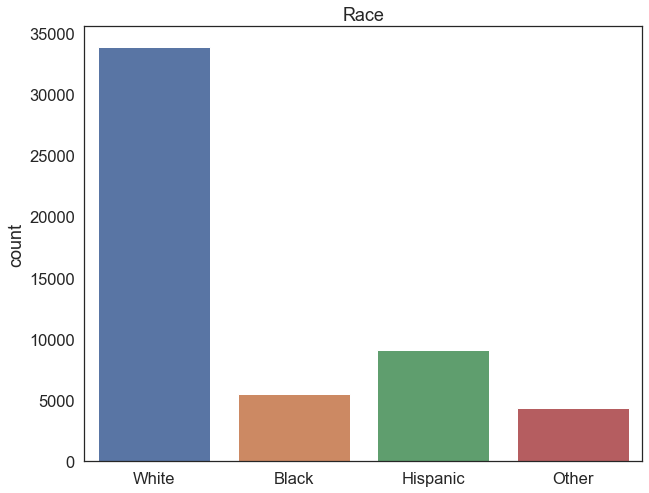
\includegraphics{notebooks/W07. Distributions and Basic Statistics_files/figure-pdf/cell-9-output-1.png}

}

\end{figure}

\begin{Shaded}
\begin{Highlighting}[]
\NormalTok{income}\OperatorTok{=}\NormalTok{df[}\StringTok{\textquotesingle{}incwage\textquotesingle{}}\NormalTok{]}\OperatorTok{/}\DecValTok{1000}

\NormalTok{plt.hist(income, bins}\OperatorTok{=}\DecValTok{100}\NormalTok{, edgecolor}\OperatorTok{=}\StringTok{\textquotesingle{}white\textquotesingle{}}\NormalTok{)}
\NormalTok{plt.xlabel(}\StringTok{\textquotesingle{}Income ($, thousands\textquotesingle{}}\NormalTok{)}
\NormalTok{plt.title(}\StringTok{"U.S. Income Distributon, 2013"}\NormalTok{)}

\NormalTok{plt.show()}
\end{Highlighting}
\end{Shaded}

\begin{figure}[H]

{\centering \includegraphics{notebooks/W07. Distributions and Basic Statistics_files/figure-pdf/cell-10-output-1.png}

}

\end{figure}

\begin{Shaded}
\begin{Highlighting}[]
\NormalTok{inc\_summary}\OperatorTok{=}\NormalTok{income.describe()}
\BuiltInTok{print}\NormalTok{(inc\_summary[[}\StringTok{\textquotesingle{}mean\textquotesingle{}}\NormalTok{,}\StringTok{\textquotesingle{}50\%\textquotesingle{}}\NormalTok{,}\StringTok{\textquotesingle{}std\textquotesingle{}}\NormalTok{]])}

\NormalTok{plt.hist(income, bins}\OperatorTok{=}\DecValTok{100}\NormalTok{, edgecolor}\OperatorTok{=}\StringTok{\textquotesingle{}white\textquotesingle{}}\NormalTok{)}
\NormalTok{plt.axvline(inc\_summary[}\StringTok{\textquotesingle{}mean\textquotesingle{}}\NormalTok{], color}\OperatorTok{=}\StringTok{\textquotesingle{}red\textquotesingle{}}\NormalTok{, linestyle}\OperatorTok{=}\StringTok{\textquotesingle{}dashed\textquotesingle{}}\NormalTok{, linewidth}\OperatorTok{=}\DecValTok{1}\NormalTok{,label}\OperatorTok{=}\StringTok{\textquotesingle{}Mean\textquotesingle{}}\NormalTok{)}
\NormalTok{plt.axvline(inc\_summary[}\StringTok{\textquotesingle{}50\%\textquotesingle{}}\NormalTok{], color}\OperatorTok{=}\StringTok{\textquotesingle{}black\textquotesingle{}}\NormalTok{, linestyle}\OperatorTok{=}\StringTok{\textquotesingle{}dashed\textquotesingle{}}\NormalTok{, linewidth}\OperatorTok{=}\DecValTok{1}\NormalTok{, label}\OperatorTok{=}\StringTok{\textquotesingle{}Median\textquotesingle{}}\NormalTok{)}

\NormalTok{plt.legend()}
\NormalTok{plt.xlabel(}\StringTok{\textquotesingle{}Income ($, thousands\textquotesingle{}}\NormalTok{)}
\NormalTok{plt.title(}\StringTok{"U.S. Income Distributon, 2013"}\NormalTok{)}
\NormalTok{plt.xlim(}\DecValTok{0}\NormalTok{,}\DecValTok{250}\NormalTok{)}
\NormalTok{plt.show()}
\end{Highlighting}
\end{Shaded}

\begin{verbatim}
mean    51.821863
50%     40.000000
std     60.163449
Name: incwage, dtype: float64
\end{verbatim}

\begin{figure}[H]

{\centering 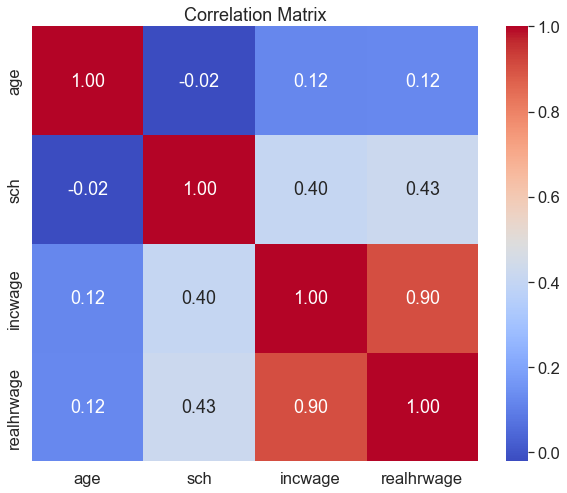
\includegraphics{notebooks/W07. Distributions and Basic Statistics_files/figure-pdf/cell-11-output-2.png}

}

\end{figure}

\begin{Shaded}
\begin{Highlighting}[]
\KeywordTok{def}\NormalTok{ plot\_histogram(variable, bins, xlab, title):}
\NormalTok{    summary}\OperatorTok{=}\NormalTok{variable.describe()}
\NormalTok{    plt.hist(variable, bins}\OperatorTok{=}\NormalTok{bins,edgecolor}\OperatorTok{=}\StringTok{\textquotesingle{}white\textquotesingle{}}\NormalTok{, density}\OperatorTok{=}\VariableTok{True}\NormalTok{)}
\NormalTok{    plt.axvline(summary[}\StringTok{\textquotesingle{}mean\textquotesingle{}}\NormalTok{], color}\OperatorTok{=}\StringTok{\textquotesingle{}red\textquotesingle{}}\NormalTok{, linestyle}\OperatorTok{=}\StringTok{\textquotesingle{}dashed\textquotesingle{}}\NormalTok{, linewidth}\OperatorTok{=}\DecValTok{1}\NormalTok{,label}\OperatorTok{=}\StringTok{\textquotesingle{}Mean \textquotesingle{}}\OperatorTok{+}\BuiltInTok{str}\NormalTok{(}\BuiltInTok{round}\NormalTok{(summary[}\StringTok{\textquotesingle{}mean\textquotesingle{}}\NormalTok{],}\DecValTok{2}\NormalTok{)))}
\NormalTok{    plt.axvline(summary[}\StringTok{\textquotesingle{}50\%\textquotesingle{}}\NormalTok{], color}\OperatorTok{=}\StringTok{\textquotesingle{}black\textquotesingle{}}\NormalTok{, linestyle}\OperatorTok{=}\StringTok{\textquotesingle{}dashed\textquotesingle{}}\NormalTok{, linewidth}\OperatorTok{=}\DecValTok{1}\NormalTok{, label}\OperatorTok{=}\StringTok{\textquotesingle{}Median \textquotesingle{}}\OperatorTok{+}\BuiltInTok{str}\NormalTok{(}\BuiltInTok{round}\NormalTok{(summary[}\StringTok{\textquotesingle{}50\%\textquotesingle{}}\NormalTok{],}\DecValTok{2}\NormalTok{)))}

\NormalTok{    plt.legend()}
\NormalTok{    plt.xlabel(xlab)}
\NormalTok{    plt.title(title)}
\NormalTok{    plt.show()}

\NormalTok{plot\_histogram(df[}\StringTok{\textquotesingle{}incwage\textquotesingle{}}\NormalTok{]}\OperatorTok{/}\DecValTok{1000}\NormalTok{, bins}\OperatorTok{=}\DecValTok{100}\NormalTok{, xlab}\OperatorTok{=}\StringTok{\textquotesingle{}Income ($, 000)\textquotesingle{}}\NormalTok{,title}\OperatorTok{=}\StringTok{\textquotesingle{}U.S. Income Distribution, 2013\textquotesingle{}}\NormalTok{)}
\end{Highlighting}
\end{Shaded}

\begin{figure}[H]

{\centering 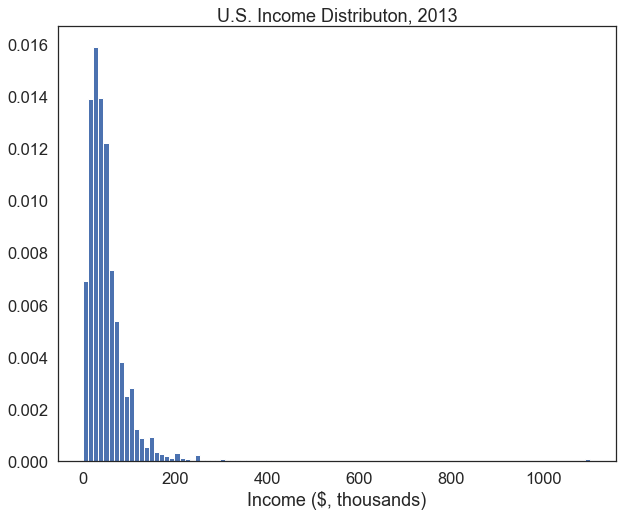
\includegraphics{notebooks/W07. Distributions and Basic Statistics_files/figure-pdf/cell-12-output-1.png}

}

\end{figure}

\begin{Shaded}
\begin{Highlighting}[]
\NormalTok{plot\_histogram(df[}\StringTok{\textquotesingle{}age\textquotesingle{}}\NormalTok{], bins}\OperatorTok{=}\DecValTok{20}\NormalTok{, xlab}\OperatorTok{=}\StringTok{\textquotesingle{}Age\textquotesingle{}}\NormalTok{,title}\OperatorTok{=}\StringTok{\textquotesingle{}U.S. Age Distribution, 2013\textquotesingle{}}\NormalTok{)}
\end{Highlighting}
\end{Shaded}

\begin{figure}[H]

{\centering 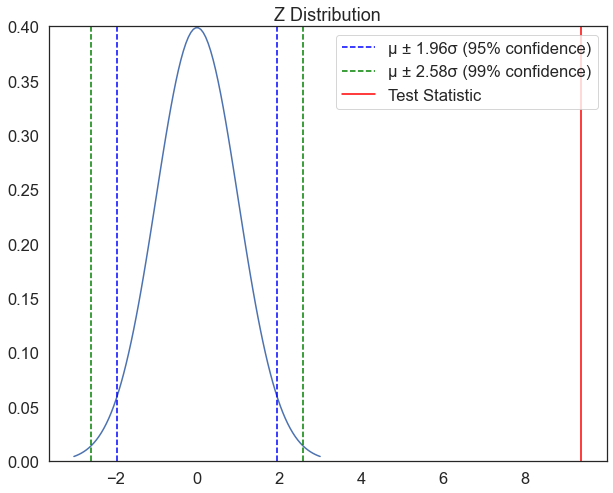
\includegraphics{notebooks/W07. Distributions and Basic Statistics_files/figure-pdf/cell-13-output-1.png}

}

\end{figure}

\begin{Shaded}
\begin{Highlighting}[]
\NormalTok{mu, se}\OperatorTok{=} \DecValTok{0}\NormalTok{, }\DecValTok{1}
\NormalTok{x }\OperatorTok{=}\NormalTok{ np.linspace(mu }\OperatorTok{{-}} \DecValTok{3}\OperatorTok{*}\NormalTok{se, mu }\OperatorTok{+} \DecValTok{3}\OperatorTok{*}\NormalTok{se, }\DecValTok{100}\NormalTok{)}
\NormalTok{plt.plot(x, norm.pdf(x, mu, se))}
\NormalTok{plt.axvline(mu, color}\OperatorTok{=}\StringTok{\textquotesingle{}black\textquotesingle{}}\NormalTok{, linestyle}\OperatorTok{=}\StringTok{\textquotesingle{}solid\textquotesingle{}}\NormalTok{, linewidth}\OperatorTok{=}\DecValTok{1}\NormalTok{,label}\OperatorTok{=}\StringTok{\textquotesingle{}µ\textquotesingle{}}\NormalTok{)}
\NormalTok{plt.axvline(mu}\OperatorTok{{-}}\NormalTok{se}\OperatorTok{*}\DecValTok{2}\NormalTok{, color}\OperatorTok{=}\StringTok{\textquotesingle{}black\textquotesingle{}}\NormalTok{, linestyle}\OperatorTok{=}\StringTok{\textquotesingle{}dashed\textquotesingle{}}\NormalTok{, linewidth}\OperatorTok{=}\FloatTok{1.5}\NormalTok{,label}\OperatorTok{=}\StringTok{\textquotesingle{}µ ± 2σ\textquotesingle{}}\NormalTok{)}
\NormalTok{plt.axvline(mu}\OperatorTok{+}\NormalTok{se}\OperatorTok{*}\DecValTok{2}\NormalTok{, color}\OperatorTok{=}\StringTok{\textquotesingle{}black\textquotesingle{}}\NormalTok{, linestyle}\OperatorTok{=}\StringTok{\textquotesingle{}dashed\textquotesingle{}}\NormalTok{, linewidth}\OperatorTok{=}\FloatTok{1.5}\NormalTok{)}
\NormalTok{plt.legend()}
\NormalTok{plt.show()}
\end{Highlighting}
\end{Shaded}

\begin{figure}[H]

{\centering 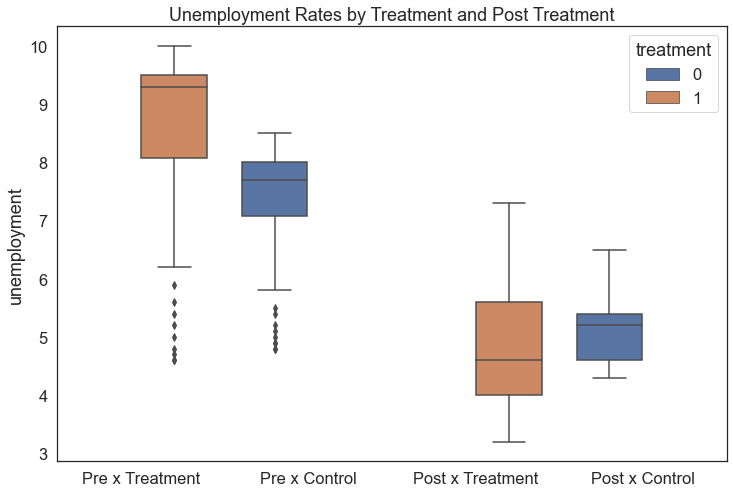
\includegraphics{notebooks/W07. Distributions and Basic Statistics_files/figure-pdf/cell-15-output-1.png}

}

\end{figure}

\begin{Shaded}
\begin{Highlighting}[]
\KeywordTok{def}\NormalTok{ plot\_sample\_means(var, xlab, sample\_size):}

    \CommentTok{\#create an empty list to store sample means}
\NormalTok{    sample\_means}\OperatorTok{=}\NormalTok{[]}

    \CommentTok{\# loop 10,000 times.}
    \ControlFlowTok{for}\NormalTok{ i }\KeywordTok{in} \BuiltInTok{range}\NormalTok{(}\DecValTok{0}\NormalTok{,}\DecValTok{10000}\NormalTok{):}
        \CommentTok{\# for each iteration, draw a sample of the size specified by the "sample\_size" parameter}
\NormalTok{        sample}\OperatorTok{=}\NormalTok{var.sample(sample\_size, replace}\OperatorTok{=}\VariableTok{True}\NormalTok{)}
        \CommentTok{\# calculate the mean, and append it to the list of sample means. }
\NormalTok{        sample\_mean}\OperatorTok{=}\NormalTok{sample.mean()}
\NormalTok{        sample\_means.append(sample\_mean)}
    
    \CommentTok{\# now, plot a histogram }
\NormalTok{    plt.hist(sample\_means, bins}\OperatorTok{=}\BuiltInTok{int}\NormalTok{(}\DecValTok{30}\NormalTok{), color}\OperatorTok{=} \StringTok{\textquotesingle{}green\textquotesingle{}}\NormalTok{, edgecolor}\OperatorTok{=}\StringTok{\textquotesingle{}white\textquotesingle{}}\NormalTok{, density}\OperatorTok{=}\VariableTok{True}\NormalTok{)}
    
    \CommentTok{\# fit a normal distribution to the data }
\NormalTok{    mu, se }\OperatorTok{=}\NormalTok{ norm.fit(sample\_means)}
\NormalTok{    xmin, xmax }\OperatorTok{=}\NormalTok{ plt.xlim()}
\NormalTok{    x }\OperatorTok{=}\NormalTok{ np.linspace(xmin, xmax, }\DecValTok{100}\NormalTok{)}
\NormalTok{    p }\OperatorTok{=}\NormalTok{ norm.pdf(x, mu, se) }
\NormalTok{    plt.plot(x, p, }\StringTok{\textquotesingle{}k\textquotesingle{}}\NormalTok{, linewidth}\OperatorTok{=}\DecValTok{2}\NormalTok{)}

    \CommentTok{\# calculate the difference between the mean of the sample means }
\NormalTok{    diff}\OperatorTok{=}\BuiltInTok{abs}\NormalTok{(mu}\OperatorTok{{-}}\NormalTok{var.mean())}
    
    \CommentTok{\# add droplines, labels, title, legend, and limit the x{-}axis range to 3 standard deviations from the mean on either side.}
\NormalTok{    plt.axvline(mu, color}\OperatorTok{=}\StringTok{\textquotesingle{}black\textquotesingle{}}\NormalTok{, linestyle}\OperatorTok{=}\StringTok{\textquotesingle{}dashed\textquotesingle{}}\NormalTok{, linewidth}\OperatorTok{=}\DecValTok{1}\NormalTok{,label}\OperatorTok{=}\StringTok{\textquotesingle{}µx̄ {-} µ= \textquotesingle{}}\OperatorTok{+}\BuiltInTok{str}\NormalTok{(}\BuiltInTok{round}\NormalTok{(diff, }\DecValTok{3}\NormalTok{)))}
\NormalTok{    plt.axvline(mu}\OperatorTok{{-}}\NormalTok{se}\OperatorTok{*}\DecValTok{2}\NormalTok{, color}\OperatorTok{=}\StringTok{\textquotesingle{}black\textquotesingle{}}\NormalTok{, linestyle}\OperatorTok{=}\StringTok{\textquotesingle{}dashed\textquotesingle{}}\NormalTok{, linewidth}\OperatorTok{=}\FloatTok{1.5}\NormalTok{,label}\OperatorTok{=}\StringTok{\textquotesingle{}µ ± 2σ\textquotesingle{}}\NormalTok{)}
\NormalTok{    plt.axvline(mu}\OperatorTok{+}\NormalTok{se}\OperatorTok{*}\DecValTok{2}\NormalTok{, color}\OperatorTok{=}\StringTok{\textquotesingle{}black\textquotesingle{}}\NormalTok{, linestyle}\OperatorTok{=}\StringTok{\textquotesingle{}dashed\textquotesingle{}}\NormalTok{, linewidth}\OperatorTok{=}\FloatTok{1.5}\NormalTok{)}
\NormalTok{    plt.legend()}
\NormalTok{    plt.xlabel(xlab)    }
\NormalTok{    plt.title(}\StringTok{\textquotesingle{}Distribution of Sample Means (n=}\SpecialCharTok{\{\}}\StringTok{)\textquotesingle{}}\NormalTok{.}\BuiltInTok{format}\NormalTok{(sample\_size))}
\NormalTok{    plt.xlim(mu}\OperatorTok{{-}}\NormalTok{se}\OperatorTok{*}\DecValTok{3}\NormalTok{, mu}\OperatorTok{+}\NormalTok{se}\OperatorTok{*}\DecValTok{3}\NormalTok{)}
\NormalTok{    plt.show()  }
\end{Highlighting}
\end{Shaded}

\begin{Shaded}
\begin{Highlighting}[]
\NormalTok{plot\_sample\_means(income, xlab}\OperatorTok{=}\StringTok{\textquotesingle{}Income, ($, 000)\textquotesingle{}}\NormalTok{, sample\_size}\OperatorTok{=}\DecValTok{2}\NormalTok{)}
\end{Highlighting}
\end{Shaded}

\begin{figure}[H]

{\centering 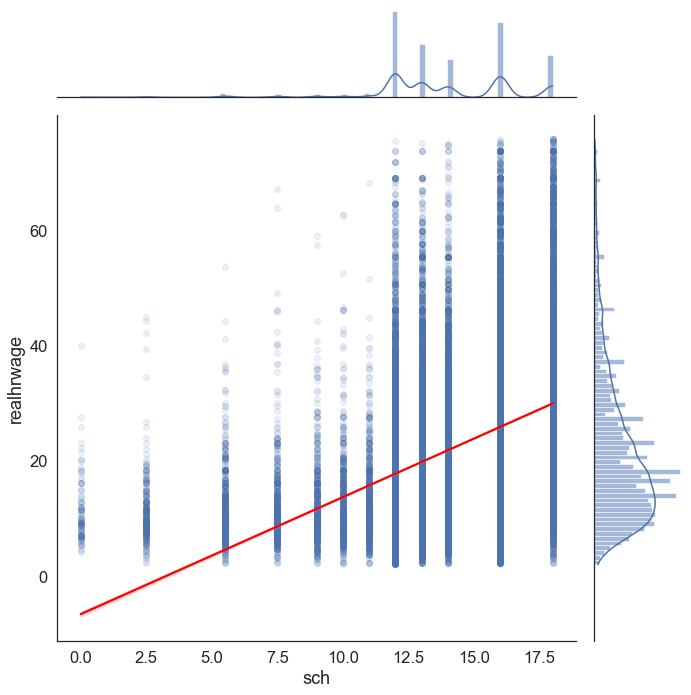
\includegraphics{notebooks/W07. Distributions and Basic Statistics_files/figure-pdf/cell-17-output-1.png}

}

\end{figure}

\begin{Shaded}
\begin{Highlighting}[]
\NormalTok{plot\_sample\_means(df[}\StringTok{\textquotesingle{}union\textquotesingle{}}\NormalTok{], xlab}\OperatorTok{=}\StringTok{\textquotesingle{}Income, ($, 000)\textquotesingle{}}\NormalTok{, sample\_size}\OperatorTok{=}\DecValTok{1000}\NormalTok{)}
\end{Highlighting}
\end{Shaded}

\begin{figure}[H]

{\centering \includegraphics{notebooks/W07. Distributions and Basic Statistics_files/figure-pdf/cell-18-output-1.png}

}

\end{figure}

\bookmarksetup{startatroot}

\hypertarget{exercise-counting-heads}{%
\chapter{Exercise: counting heads}\label{exercise-counting-heads}}

By modifying variables in the code above, create and plot a distribution
of heights for \emph{men} in the USA. Use of wikipedia and the internet
is allowed. Social media is not.

How many men in America are average height? (Hint: think about the
``sample'' variable)

\emph{Extension:} How many men in the USA are within 7cm of the mean?

\bookmarksetup{startatroot}

\hypertarget{in-the-bin}{%
\chapter{In the bin}\label{in-the-bin}}

Slightly more subtly, the bin size might affect our answers to some of
these questions. In order to create a distribution, we need to
\emph{bin} data to create the graph that we've created - a
\emph{histogram} which we expect to reflect the probability mass
function. If I give you a string of heights (1.1, 1.5, 1.6, 1.2, 1.8,
1.4, 1.0, 1.55, 1.74, etc) you can probably see that they cluster around
1.5 or thereabouts, but to graph them as a histogram, you need to choose
a bin size and range. Let's say we choose 10 bins, starting at 1m and
each bin is 0.1m bigger. So if the height h is 1.0 \(\leq\) h
\textless{} 1.1, it goes into the first bin, if 1.1 \(\leq\) h
\textless{} 1.2 in the second and so on. For this data, we'd see one
entry in the first bin, one in the second, a few around the middle and
only one in the higher echelons.

This is pretty basic and you're probably familiar with it. But you need
to choose the number of bins appropriately for the data set - and that's
very sensitive to the number of samples you have.

\bookmarksetup{startatroot}

\hypertarget{exercise-keep-gaussians-tidy}{%
\chapter{Exercise: Keep Gaussians
Tidy}\label{exercise-keep-gaussians-tidy}}

In the above code, increase the number of bins to 1000 - what do you
notice?

Reduce the number of bins to 10 - what happens now? What's causing this
effect?

Reduce the number of samples to 1000. What affect does this have on the
histogram?

How can you use this information for plotting and binning data?

\emph{Extension}: to find more about the function used to sample these
random numbers above, take a look at the Python documentation:
http://docs.scipy.org/doc/numpy/reference/generated/numpy.random.randn.html)

\bookmarksetup{startatroot}

\hypertarget{some-normal-behaviours}{%
\chapter{Some Normal Behaviours}\label{some-normal-behaviours}}

Let's look at the mean and standard deviation on the graph. We can
calculate the mean and standard deviation of our (synthetic) dataset a
by using the np.mean() and np.std() methods.

Recall that the . notation means we're using a method from ``inside''
the numpy library.

\begin{Shaded}
\begin{Highlighting}[]
\CommentTok{\#as we did before...}
\NormalTok{plt.hist(heights, bins, histtype}\OperatorTok{=}\StringTok{\textquotesingle{}step\textquotesingle{}}\NormalTok{)}
\CommentTok{\#draw the mean}
\NormalTok{plt.axvline(numpy.mean(heights), color }\OperatorTok{=} \StringTok{\textquotesingle{}r\textquotesingle{}}\NormalTok{)}
\NormalTok{sd }\OperatorTok{=}\NormalTok{ numpy.std(heights)}
\CommentTok{\#draw mean + one s.d.}
\NormalTok{plt.axvline(numpy.mean(heights) }\OperatorTok{+}\NormalTok{ sd, color}\OperatorTok{=}\StringTok{\textquotesingle{}k\textquotesingle{}}\NormalTok{)}
\CommentTok{\#draw mean {-} one s.d.}
\NormalTok{plt.axvline(numpy.mean(heights) }\OperatorTok{{-}}\NormalTok{ sd, color }\OperatorTok{=} \StringTok{\textquotesingle{}k\textquotesingle{}}\NormalTok{)}
\NormalTok{plt.xlabel(}\StringTok{\textquotesingle{}Height [cm]\textquotesingle{}}\NormalTok{)}
\NormalTok{plt.ylabel(}\StringTok{\textquotesingle{}Frequency\textquotesingle{}}\NormalTok{)}
\NormalTok{plt.title(}\StringTok{\textquotesingle{}Fake Heights\textquotesingle{}}\NormalTok{)}
\end{Highlighting}
\end{Shaded}

\begin{verbatim}
NameError: name 'heights' is not defined
\end{verbatim}

Gaussians have some nice standard properties - for example, 68\% of the
data lies within one standard deviation of the mean. That means in our
example above, 2/3 of women in the UK are between 1.57m and 1.69m tall.
With a Gaussian, 95\% of data is within two standard deviations - so
95\% of women in the UK are at least 1.51m tall, and shorter than 1.75m.
So this starts to answer some of our questions we posed initially - from
a random sample, there is a 1 in 40 chance of a woman in the uk being
taller than 1.75m. \textbf{How did I arrive at that figure?}

Let's also plot the \emph{median} of the Gaussian:

\begin{Shaded}
\begin{Highlighting}[]
\CommentTok{\#as we did before...}
\NormalTok{plt.hist(heights, bins, histtype}\OperatorTok{=}\StringTok{\textquotesingle{}step\textquotesingle{}}\NormalTok{)}
\CommentTok{\#draw the median}
\NormalTok{plt.axvline(numpy.median(heights), color }\OperatorTok{=} \StringTok{\textquotesingle{}g\textquotesingle{}}\NormalTok{)}
\NormalTok{plt.xlabel(}\StringTok{\textquotesingle{}Height [cm]\textquotesingle{}}\NormalTok{)}
\NormalTok{plt.ylabel(}\StringTok{\textquotesingle{}Frequency\textquotesingle{}}\NormalTok{)}
\NormalTok{plt.title(}\StringTok{\textquotesingle{}Fake Heights\textquotesingle{}}\NormalTok{)}
\end{Highlighting}
\end{Shaded}

\begin{verbatim}
Text(0.5, 1.0, 'Fake Heights')
\end{verbatim}

\begin{figure}[H]

{\centering \includegraphics{notebooks/W07. Distributions and Basic Statistics_files/figure-pdf/cell-24-output-2.png}

}

\end{figure}

\bookmarksetup{startatroot}

\hypertarget{question}{%
\chapter{Question:}\label{question}}

Why is the mean the same as the mean (and the mode)?

Not all probability distributions follow the same logic, though -
sometimes a sample is possible - even likely - even if it is dozens of
times the mean, which for height would be tens of metres tall. More
generally, we can start to unpick the shape of a probability curve using
\emph{moments}.

\bookmarksetup{startatroot}

\hypertarget{asymmetric-distributions}{%
\chapter{Asymmetric Distributions}\label{asymmetric-distributions}}

We won't talk about how we decide what the best fit for a dataset is -
suffice it to say that a Gaussian doesn't always fit the bill. In those
cases, the general curve we're dealing with will have a more complex
form.

(\emph{Sometimes we can know that from the underlying process generating
the data - other times we don't, and it's analysing the shape of the
data that tells us})

\begin{Shaded}
\begin{Highlighting}[]
\NormalTok{x\_val}\OperatorTok{=}\NormalTok{ numpy.linspace(}\DecValTok{0}\NormalTok{,}\DecValTok{15}\NormalTok{,}\DecValTok{100}\NormalTok{)}
\NormalTok{y\_val }\OperatorTok{=}\NormalTok{ (x\_val}\OperatorTok{**}\DecValTok{3}\NormalTok{)}\OperatorTok{*}\NormalTok{numpy.exp(}\OperatorTok{{-}}\NormalTok{x\_val)}
\NormalTok{plt.plot(x\_val,y\_val)}
\NormalTok{plt.xlabel(}\StringTok{\textquotesingle{}Value\textquotesingle{}}\NormalTok{)}
\NormalTok{plt.ylabel(}\StringTok{\textquotesingle{}Frequency\textquotesingle{}}\NormalTok{)}
\end{Highlighting}
\end{Shaded}

\begin{verbatim}
Text(0, 0.5, 'Frequency')
\end{verbatim}

\begin{figure}[H]

{\centering 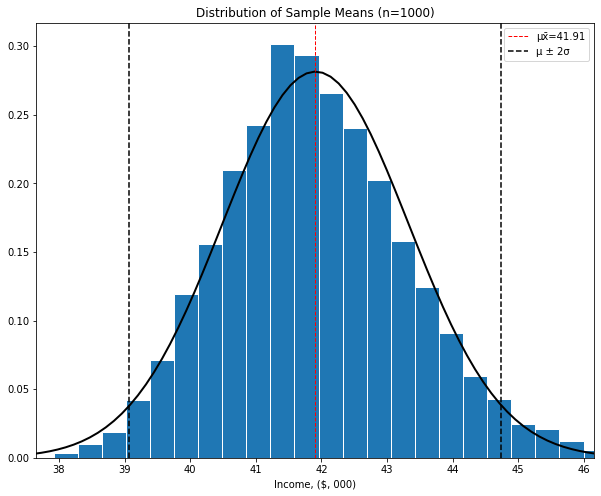
\includegraphics{notebooks/W07. Distributions and Basic Statistics_files/figure-pdf/cell-26-output-2.png}

}

\end{figure}

How do we characterise a dataset which is complex, asymmetric, or we
don't know the underlying form?

\bookmarksetup{startatroot}

\hypertarget{magic-moments}{%
\chapter{Magic Moments}\label{magic-moments}}

Without going into the mathematical detail yet, you can think about
moments as being increasingly nuanced ways of describing distributions.
There are an infinite number of them, but you can understand the first
few inituitively.

\hypertarget{th-moment}{%
\section{0th moment}\label{th-moment}}

0th moment is just area under the curve. In this case it would just be
the number of people sampled. It doesn't tell us much.

\hypertarget{st-moment}{%
\section{1st moment}\label{st-moment}}

1st moment is a central ``tendency'' or average value of the
distribution. In a Gaussian, the mean (average) \(\mu\) is the average
and the centre. But there are other ways of representing this
characteristic, like mode or median, as we will see.

\hypertarget{nd-moment}{%
\section{2nd moment}\label{nd-moment}}

Second moment represents the \emph{width} or \emph{spread} of the curve.
\(\sigma\) is calculated from the second moment, and in a Gaussian
represents the width of the curve. Interquartile range is another way of
doing this, or half-life.

\hypertarget{rd-moment}{%
\section{3rd moment}\label{rd-moment}}

The third moment is related to how \emph{asymmetrical} a curve is, and
the usual way to quantify this is \emph{skewness}. A Gaussian is
symmetric, so its skewness is zero. Actually, all moments apart from 0,
1 and 2 are zero for a Gaussian.

\hypertarget{th-moment-1}{%
\section{4th moment}\label{th-moment-1}}

The standard way to calculate a fourth moment is \emph{Kurtosis}. This
is a measure of how ``peaky'' or ``taily'' a curve is. It's a bit harder
to visualise what we're on about at this point, but it's worth
remembering that a Gaussian has a Kurtosis of 0, so isn't very
``taily''.

\hypertarget{other-moments}{%
\section{Other moments}\label{other-moments}}

It's harder to interpret what they mean, but an arbitrary probability
distribution may need an \emph{infinite} series of moments to be
described correctly. Gaussians are unusual in that they require only two
parameters to describe them; if your data looks Gaussian, that makes
life easier in many ways.

\textbf{Extension}: there are distributions which are simple to write
down that nevertheless are described by an infinite series of moments;
and some, like the Lorentzian, are quite nice functions that have
infinite values for most of their moments.

\hypertarget{recap-the-median}{%
\section{Recap: The Median}\label{recap-the-median}}

The \emph{median} is different from the mean. The median of a data set
is an element that seperates the higher half of the data from the lower
half. For example, the median of \(A = \left \{1,2,3,4,5\right \}\) is
3, and 3 is also the median of \(B = \left \{1,2,3,9,10\right \}\). When
a data set has an even number of members like
\(C = \left \{1,2,3,4\right \}\), the median is defined as the average
of the top lower half and the lower top half, so the median of C is
(2+3)/2=2.5 .

\textbf{Advanced}: How did we define the median from a distribution
(hint: consider area under curve and what it means)? What about
quartiles? What about deciles? What are these quantities?

\hypertarget{exercise-18}{%
\section{Exercise}\label{exercise-18}}

Under which conditions is the median equal to the mean? (hint: look at
the normal distribution - but think more broadly abouting how
``counting'' and ``area under curve'' are related in histograms).

\hypertarget{exercise-19}{%
\section{Exercise}\label{exercise-19}}

Construct a set of 5 numbers such that the median is half the value of
the mean.

\hypertarget{power-laws}{%
\section{Power Laws}\label{power-laws}}

Another type of important distributions are \textbf{power law}
distributions. When the probability of a variable to take the value of
\(x\) is roughly \(\frac{1}{x^k}\) we say that \(x\) has a power law
distribution with exponent \(k\).

For instance let's plot a power law function with exponent 3.

We start off by generating an array of 100 numbers between 1 and 10;
numpy.linspace() lets us do this (here is the documentation if you want
to find out more:
http://docs.scipy.org/doc/numpy/reference/generated/numpy.linspace.html)

\begin{Shaded}
\begin{Highlighting}[]
\NormalTok{x\_val}\OperatorTok{=}\NormalTok{ numpy.linspace(}\DecValTok{1}\NormalTok{,}\DecValTok{10}\NormalTok{,}\DecValTok{100}\NormalTok{)}
\CommentTok{\#** is "to the power of" in Pythonese}
\NormalTok{y\_val }\OperatorTok{=} \DecValTok{1}\OperatorTok{/}\NormalTok{x\_val}\OperatorTok{**}\DecValTok{3}
\NormalTok{plt.plot(x\_val,y\_val)}
\NormalTok{plt.xlabel(}\StringTok{\textquotesingle{}Value\textquotesingle{}}\NormalTok{)}
\NormalTok{plt.ylabel(}\StringTok{\textquotesingle{}Frequency\textquotesingle{}}\NormalTok{)}
\NormalTok{plt.xlim(}\DecValTok{1}\NormalTok{,}\DecValTok{5}\NormalTok{)}
\end{Highlighting}
\end{Shaded}

\begin{verbatim}
(1.0, 5.0)
\end{verbatim}

\begin{figure}[H]

{\centering \includegraphics{notebooks/W07. Distributions and Basic Statistics_files/figure-pdf/cell-29-output-2.png}

}

\end{figure}

An important class of power law distributions are called \textbf{Pareto}
type distributions. Consider for instance, the distribution of income in
a city. We will find that about 20\% of the population has 80\% of the
wealth, this is also known as a 80:20 law.

\begin{Shaded}
\begin{Highlighting}[]
\NormalTok{sample }\OperatorTok{=} \DecValTok{10000}
\NormalTok{exponent }\OperatorTok{=} \DecValTok{3}

\NormalTok{bins }\OperatorTok{=} \DecValTok{1000}


\NormalTok{y }\OperatorTok{=} \DecValTok{1} \OperatorTok{+}\NormalTok{ numpy.random.pareto(exponent, sample)}

\NormalTok{plt.hist(y, bins, histtype}\OperatorTok{=}\StringTok{\textquotesingle{}step\textquotesingle{}}\NormalTok{)}
\NormalTok{plt.xlim((}\DecValTok{1}\NormalTok{, }\DecValTok{5}\NormalTok{))}
\NormalTok{plt.xlabel(}\StringTok{\textquotesingle{}Value\textquotesingle{}}\NormalTok{)}
\NormalTok{plt.ylabel(}\StringTok{\textquotesingle{}Frequency\textquotesingle{}}\NormalTok{)}
\end{Highlighting}
\end{Shaded}

\begin{verbatim}
Text(0, 0.5, 'Frequency')
\end{verbatim}

\begin{figure}[H]

{\centering \includegraphics{notebooks/W07. Distributions and Basic Statistics_files/figure-pdf/cell-30-output-2.png}

}

\end{figure}

\hypertarget{exercise-20}{%
\section{Exercise:}\label{exercise-20}}

Add lines showing the mean, mode and median to the above graph, and
comment on this with a box of markdown.

\hypertarget{comments}{%
\section{Comments:}\label{comments}}

We plotted the mean, mode and median of the distribution\ldots{}

\hypertarget{extension-quantifying-datasets-which-cover-a-wide-range-of-values.}{%
\section{Extension: Quantifying Datasets Which Cover a Wide Range of
Values.}\label{extension-quantifying-datasets-which-cover-a-wide-range-of-values.}}

Objects like the mean present a problem for power laws - in some cases,
they diverge. So, for the mathematicians, if the exponent is 1, we can
approximate the mean by

\(\mu = \int_0^{\infty}dx \frac{1}{x}*x = \int_0^{\infty}dx = \infty\)!

which gives a nonsensical value. Larger exponents (larger than 2) ensure
this doesn't occur - but what sense does the mean make when there are
people earning 10, 100 or 1000 times that mean value?

When datasets cover many orders of magnitude (here from 33 to 2090), we
may need to think about \emph{geometrical} methods for understanding its
properties. For the mean, we might consider the \emph{geometrical mean},
achieved by mutiplying the 100 values together and taking the 100th
root. To understand the width, we might use a half-life type measure.
Half-life is the ``time'' it takes for a radioactive source to reach
half its current level of radioactivity; but we can think about applying
this to other situations, where ``time'' is replaced by ``percentile''
and ``radioactivity'' is replaced by ``income'', for example.

\hypertarget{extension-bimodal-distributions}{%
\section{Extension: Bimodal
Distributions}\label{extension-bimodal-distributions}}

Sometimes distributions are \emph{Bimodal} or multimodal. What this
literally means is that they have multiple ``modes'' - most popular
values - i.e.~peaks. In these cases, mean may not be the best measure
and we may need to think about these two (or larger number of) peaks
relates to different segments of our sample or population.

\begin{Shaded}
\begin{Highlighting}[]
\NormalTok{sample }\OperatorTok{=} \DecValTok{100000}
\NormalTok{a }\OperatorTok{=} \DecValTok{25} \OperatorTok{*}\NormalTok{ numpy.random.randn(sample) }\OperatorTok{+} \DecValTok{20}
\ControlFlowTok{for}\NormalTok{ i }\KeywordTok{in} \BuiltInTok{range}\NormalTok{(}\BuiltInTok{int}\NormalTok{(sample}\OperatorTok{/}\DecValTok{2}\NormalTok{)):}
\NormalTok{    a[i] }\OperatorTok{=}\NormalTok{ a[i]}\OperatorTok{*}\FloatTok{1.3}\OperatorTok{+}\DecValTok{100}
\NormalTok{plt.hist(a, }\DecValTok{250}\NormalTok{, histtype}\OperatorTok{=}\StringTok{\textquotesingle{}step\textquotesingle{}}\NormalTok{)}\OperatorTok{;}
\NormalTok{plt.xlabel(}\StringTok{\textquotesingle{}Value\textquotesingle{}}\NormalTok{)}
\NormalTok{plt.ylabel(}\StringTok{\textquotesingle{}Frequency\textquotesingle{}}\NormalTok{)}
\end{Highlighting}
\end{Shaded}

\begin{verbatim}
Text(0, 0.5, 'Frequency')
\end{verbatim}

\begin{figure}[H]

{\centering \includegraphics{notebooks/W07. Distributions and Basic Statistics_files/figure-pdf/cell-33-output-2.png}

}

\end{figure}

\hypertarget{exercise-21}{%
\section{Exercise:}\label{exercise-21}}

Plot the mean and median for the above graph. What might be better
statistics? How might you find them?

\bookmarksetup{startatroot}

\hypertarget{regression}{%
\chapter{Regression}\label{regression}}

\bookmarksetup{startatroot}

\hypertarget{machine-learning}{%
\chapter{Machine Learning}\label{machine-learning}}

\hypertarget{workshop-9-open-in-colab}{%
\section[\emph{Workshop 9} ]{\texorpdfstring{\emph{Workshop 9}
\href{https://colab.research.google.com/github/oballinger/QM2/blob/main/notebooks/W09.\%20Machine\%20Learning.ipynb}{\protect
\includegraphics{notebooks/../colab-badge.png}}}{Workshop 9 Open In Colab}}\label{workshop-9-open-in-colab}}

This short introduction uses
\href{https://www.tensorflow.org/guide/keras/overview}{Keras} to:

\begin{enumerate}
\def\labelenumi{\arabic{enumi}.}
\tightlist
\item
  Load a prebuilt dataset.
\item
  Build a neural network machine learning model that classifies images.
\item
  Train this neural network.
\item
  Evaluate the accuracy of the model.
\end{enumerate}

\hypertarget{set-up-tensorflow}{%
\section{Set up TensorFlow}\label{set-up-tensorflow}}

Import TensorFlow into your program to get started:

\begin{Shaded}
\begin{Highlighting}[]
\ImportTok{import}\NormalTok{ numpy }\ImportTok{as}\NormalTok{ np}
\ImportTok{import}\NormalTok{ tensorflow }\ImportTok{as}\NormalTok{ tf}
\ImportTok{import}\NormalTok{ matplotlib.pyplot }\ImportTok{as}\NormalTok{ plt}

\BuiltInTok{print}\NormalTok{(}\StringTok{"TensorFlow version:"}\NormalTok{, tf.\_\_version\_\_)}
\end{Highlighting}
\end{Shaded}

\begin{verbatim}
TypeError: Descriptors cannot not be created directly.
If this call came from a _pb2.py file, your generated code is out of date and must be regenerated with protoc >= 3.19.0.
If you cannot immediately regenerate your protos, some other possible workarounds are:
 1. Downgrade the protobuf package to 3.20.x or lower.
 2. Set PROTOCOL_BUFFERS_PYTHON_IMPLEMENTATION=python (but this will use pure-Python parsing and will be much slower).

More information: https://developers.google.com/protocol-buffers/docs/news/2022-05-06#python-updates
\end{verbatim}

If you are following along in your own development environment, rather
than
\href{https://colab.research.google.com/github/tensorflow/docs/blob/master/site/en/tutorials/quickstart/beginner.ipynb}{Colab},
see the \href{https://www.tensorflow.org/install}{install guide} for
setting up TensorFlow for development.

Note: Make sure you have upgraded to the latest \texttt{pip} to install
the TensorFlow 2 package if you are using your own development
environment. See the \href{https://www.tensorflow.org/install}{install
guide} for details.

\hypertarget{load-a-dataset}{%
\section{Load a dataset}\label{load-a-dataset}}

Load and prepare the \href{http://yann.lecun.com/exdb/mnist/}{MNIST
dataset}. Convert the sample data from integers to floating-point
numbers:

\begin{Shaded}
\begin{Highlighting}[]
\NormalTok{mnist }\OperatorTok{=}\NormalTok{ tf.keras.datasets.mnist}

\NormalTok{(x\_train, y\_train), (x\_test, y\_test) }\OperatorTok{=}\NormalTok{ mnist.load\_data()}
\NormalTok{x\_train, x\_test }\OperatorTok{=}\NormalTok{ x\_train }\OperatorTok{/} \FloatTok{255.0}\NormalTok{, x\_test }\OperatorTok{/} \FloatTok{255.0}
\end{Highlighting}
\end{Shaded}

\begin{verbatim}
Downloading data from https://storage.googleapis.com/tensorflow/tf-keras-datasets/mnist.npz
11493376/11490434 [==============================] - 0s 0us/step
11501568/11490434 [==============================] - 0s 0us/step
\end{verbatim}

\begin{Shaded}
\begin{Highlighting}[]

\KeywordTok{def}\NormalTok{ plot\_num(number):}

\NormalTok{  item\_index }\OperatorTok{=}\NormalTok{ np.where(y\_train[:}\DecValTok{1000}\NormalTok{]}\OperatorTok{==}\NormalTok{number)}
\NormalTok{  subset}\OperatorTok{=}\NormalTok{x\_train[item\_index]}
  
\NormalTok{  egs}\OperatorTok{=}\DecValTok{5}
\NormalTok{  fig, axs }\OperatorTok{=}\NormalTok{ plt.subplots(}\DecValTok{1}\NormalTok{,egs, figsize}\OperatorTok{=}\NormalTok{(}\DecValTok{20}\NormalTok{,}\DecValTok{10}\NormalTok{))}

  \ControlFlowTok{for}\NormalTok{ i }\KeywordTok{in} \BuiltInTok{range}\NormalTok{(}\DecValTok{0}\NormalTok{,egs):}
\NormalTok{    axs[i].imshow(subset[i])}


\ControlFlowTok{for}\NormalTok{ x }\KeywordTok{in} \BuiltInTok{range}\NormalTok{(}\DecValTok{0}\NormalTok{,}\DecValTok{10}\NormalTok{):}
\NormalTok{  plot\_num(x)}
\end{Highlighting}
\end{Shaded}

\begin{figure}[H]

{\centering \includegraphics{notebooks/W09. Machine Learning_files/figure-pdf/cell-4-output-1.png}

}

\end{figure}

\begin{figure}[H]

{\centering 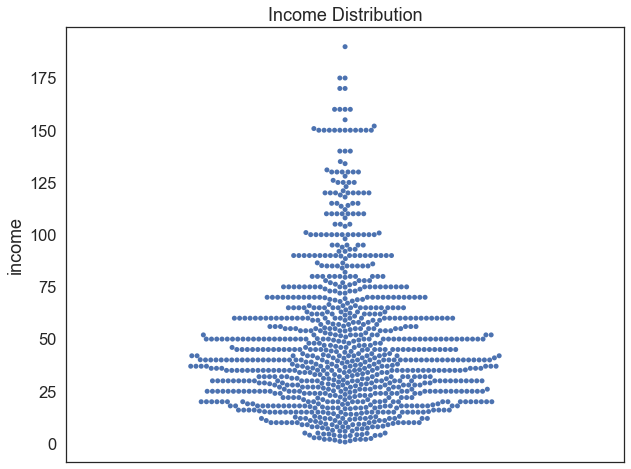
\includegraphics{notebooks/W09. Machine Learning_files/figure-pdf/cell-4-output-2.png}

}

\end{figure}

\begin{figure}[H]

{\centering \includegraphics{notebooks/W09. Machine Learning_files/figure-pdf/cell-4-output-3.png}

}

\end{figure}

\begin{figure}[H]

{\centering \includegraphics{notebooks/W09. Machine Learning_files/figure-pdf/cell-4-output-4.png}

}

\end{figure}

\begin{figure}[H]

{\centering \includegraphics{notebooks/W09. Machine Learning_files/figure-pdf/cell-4-output-5.png}

}

\end{figure}

\begin{figure}[H]

{\centering \includegraphics{notebooks/W09. Machine Learning_files/figure-pdf/cell-4-output-6.png}

}

\end{figure}

\begin{figure}[H]

{\centering \includegraphics{notebooks/W09. Machine Learning_files/figure-pdf/cell-4-output-7.png}

}

\end{figure}

\begin{figure}[H]

{\centering \includegraphics{notebooks/W09. Machine Learning_files/figure-pdf/cell-4-output-8.png}

}

\end{figure}

\begin{figure}[H]

{\centering \includegraphics{notebooks/W09. Machine Learning_files/figure-pdf/cell-4-output-9.png}

}

\end{figure}

\begin{figure}[H]

{\centering \includegraphics{notebooks/W09. Machine Learning_files/figure-pdf/cell-4-output-10.png}

}

\end{figure}

\hypertarget{build-a-machine-learning-model}{%
\section{Build a machine learning
model}\label{build-a-machine-learning-model}}

Build a \texttt{tf.keras.Sequential} model by stacking layers.

\begin{Shaded}
\begin{Highlighting}[]
\NormalTok{model }\OperatorTok{=}\NormalTok{ tf.keras.models.Sequential([}
\NormalTok{  tf.keras.layers.Flatten(input\_shape}\OperatorTok{=}\NormalTok{(}\DecValTok{28}\NormalTok{, }\DecValTok{28}\NormalTok{)),}
\NormalTok{  tf.keras.layers.Dense(}\DecValTok{128}\NormalTok{, activation}\OperatorTok{=}\StringTok{\textquotesingle{}relu\textquotesingle{}}\NormalTok{),}
\NormalTok{  tf.keras.layers.Dropout(}\FloatTok{0.2}\NormalTok{),}
\NormalTok{  tf.keras.layers.Dense(}\DecValTok{10}\NormalTok{)}
\NormalTok{])}
\end{Highlighting}
\end{Shaded}

For each example, the model returns a vector of
\href{https://developers.google.com/machine-learning/glossary\#logits}{logits}
or
\href{https://developers.google.com/machine-learning/glossary\#log-odds}{log-odds}
scores, one for each class.

\begin{Shaded}
\begin{Highlighting}[]
\NormalTok{predictions }\OperatorTok{=}\NormalTok{ model(x\_train[:}\DecValTok{1}\NormalTok{]).numpy()}
\NormalTok{predictions}
\end{Highlighting}
\end{Shaded}

\begin{verbatim}
array([[ 0.33447966,  0.35151538, -0.35632688, -0.2735348 ,  0.8568236 ,
        -0.8503612 , -0.34408805, -0.40424255,  0.4791569 , -0.00873779]],
      dtype=float32)
\end{verbatim}

The \texttt{tf.nn.softmax} function converts these logits to
\emph{probabilities} for each class:

\begin{Shaded}
\begin{Highlighting}[]
\NormalTok{tf.nn.softmax(predictions).numpy()}
\end{Highlighting}
\end{Shaded}

\begin{verbatim}
array([[0.12650587, 0.12867945, 0.06340117, 0.0688737 , 0.21328573,
        0.03868484, 0.06418189, 0.06043489, 0.1461986 , 0.08975388]],
      dtype=float32)
\end{verbatim}

Note: It is possible to bake the \texttt{tf.nn.softmax} function into
the activation function for the last layer of the network. While this
can make the model output more directly interpretable, this approach is
discouraged as it's impossible to provide an exact and numerically
stable loss calculation for all models when using a softmax output.

Define a loss function for training using
\texttt{losses.SparseCategoricalCrossentropy}, which takes a vector of
logits and a \texttt{True} index and returns a scalar loss for each
example.

\begin{Shaded}
\begin{Highlighting}[]
\NormalTok{loss\_fn }\OperatorTok{=}\NormalTok{ tf.keras.losses.SparseCategoricalCrossentropy(from\_logits}\OperatorTok{=}\VariableTok{True}\NormalTok{)}
\end{Highlighting}
\end{Shaded}

This loss is equal to the negative log probability of the true class:
The loss is zero if the model is sure of the correct class.

This untrained model gives probabilities close to random (1/10 for each
class), so the initial loss should be close to
\texttt{-tf.math.log(1/10)\ \textasciitilde{}=\ 2.3}.

\begin{Shaded}
\begin{Highlighting}[]
\NormalTok{loss\_fn(y\_train[:}\DecValTok{1}\NormalTok{], predictions).numpy()}
\end{Highlighting}
\end{Shaded}

\begin{verbatim}
3.2523074
\end{verbatim}

Before you start training, configure and compile the model using Keras
\texttt{Model.compile}. Set the
\href{https://www.tensorflow.org/api_docs/python/tf/keras/optimizers}{\texttt{optimizer}}
class to \texttt{adam}, set the \texttt{loss} to the \texttt{loss\_fn}
function you defined earlier, and specify a metric to be evaluated for
the model by setting the \texttt{metrics} parameter to
\texttt{accuracy}.

\begin{Shaded}
\begin{Highlighting}[]
\NormalTok{model.}\BuiltInTok{compile}\NormalTok{(optimizer}\OperatorTok{=}\StringTok{\textquotesingle{}adam\textquotesingle{}}\NormalTok{,}
\NormalTok{              loss}\OperatorTok{=}\NormalTok{loss\_fn,}
\NormalTok{              metrics}\OperatorTok{=}\NormalTok{[}\StringTok{\textquotesingle{}accuracy\textquotesingle{}}\NormalTok{])}
\end{Highlighting}
\end{Shaded}

\hypertarget{train-and-evaluate-your-model}{%
\section{Train and evaluate your
model}\label{train-and-evaluate-your-model}}

Use the \texttt{Model.fit} method to adjust your model parameters and
minimize the loss:

\begin{Shaded}
\begin{Highlighting}[]
\NormalTok{model.fit(x\_train, y\_train, epochs}\OperatorTok{=}\DecValTok{10}\NormalTok{)}
\end{Highlighting}
\end{Shaded}

\begin{verbatim}
Epoch 1/10
1875/1875 [==============================] - 6s 3ms/step - loss: 0.2955 - accuracy: 0.9139
Epoch 2/10
1875/1875 [==============================] - 5s 3ms/step - loss: 0.1416 - accuracy: 0.9578
Epoch 3/10
1875/1875 [==============================] - 5s 3ms/step - loss: 0.1072 - accuracy: 0.9676
Epoch 4/10
1875/1875 [==============================] - 5s 3ms/step - loss: 0.0874 - accuracy: 0.9727
Epoch 5/10
1875/1875 [==============================] - 5s 3ms/step - loss: 0.0734 - accuracy: 0.9772
Epoch 6/10
1875/1875 [==============================] - 5s 3ms/step - loss: 0.0632 - accuracy: 0.9792
Epoch 7/10
1875/1875 [==============================] - 5s 3ms/step - loss: 0.0575 - accuracy: 0.9808
Epoch 8/10
1875/1875 [==============================] - 5s 3ms/step - loss: 0.0526 - accuracy: 0.9825
Epoch 9/10
1875/1875 [==============================] - 5s 3ms/step - loss: 0.0460 - accuracy: 0.9853
Epoch 10/10
1875/1875 [==============================] - 5s 3ms/step - loss: 0.0437 - accuracy: 0.9858
\end{verbatim}

\begin{verbatim}
<keras.callbacks.History at 0x7fe943384b10>
\end{verbatim}

The \texttt{Model.evaluate} method checks the models performance,
usually on a
``\href{https://developers.google.com/machine-learning/glossary\#validation-set}{Validation-set}''
or
``\href{https://developers.google.com/machine-learning/glossary\#test-set}{Test-set}''.

\begin{Shaded}
\begin{Highlighting}[]
\NormalTok{model.evaluate(x\_test,  y\_test, verbose}\OperatorTok{=}\DecValTok{2}\NormalTok{)}
\end{Highlighting}
\end{Shaded}

\begin{verbatim}
313/313 - 1s - loss: 0.0715 - accuracy: 0.9785 - 529ms/epoch - 2ms/step
\end{verbatim}

\begin{verbatim}
[0.07152838259935379, 0.9785000085830688]
\end{verbatim}

The image classifier is now trained to \textasciitilde98\% accuracy on
this dataset. To learn more, read the
\href{https://www.tensorflow.org/tutorials/}{TensorFlow tutorials}.

If you want your model to return a probability, you can wrap the trained
model, and attach the softmax to it:

\begin{Shaded}
\begin{Highlighting}[]
\NormalTok{probability\_model }\OperatorTok{=}\NormalTok{ tf.keras.Sequential([}
\NormalTok{  model,}
\NormalTok{  tf.keras.layers.Softmax()}
\NormalTok{])}
\end{Highlighting}
\end{Shaded}

\begin{Shaded}
\begin{Highlighting}[]
\CommentTok{\#probability\_model(x\_test[:1])}
\NormalTok{predictions}\OperatorTok{=}\NormalTok{probability\_model.predict(x\_test)}

\NormalTok{index}\OperatorTok{=}\DecValTok{20}

\BuiltInTok{print}\NormalTok{(np.argmax(predictions[index]))}
\NormalTok{plt.imshow(x\_test[index])}
\end{Highlighting}
\end{Shaded}

\begin{verbatim}
9
\end{verbatim}

\begin{verbatim}
<matplotlib.image.AxesImage at 0x7fe9409c1ad0>
\end{verbatim}

\begin{figure}[H]

{\centering \includegraphics{notebooks/W09. Machine Learning_files/figure-pdf/cell-14-output-3.png}

}

\end{figure}

\hypertarget{conclusion}{%
\section{Conclusion}\label{conclusion}}

Congratulations! You have trained a machine learning model using a
prebuilt dataset using the
\href{https://www.tensorflow.org/guide/keras/overview}{Keras} API.

For more examples of using Keras, check out the
\href{https://www.tensorflow.org/tutorials/keras/}{tutorials}. To learn
more about building models with Keras, read the
\href{https://www.tensorflow.org/guide/keras}{guides}. If you want learn
more about loading and preparing data, see the tutorials on
\href{https://www.tensorflow.org/tutorials/load_data/images}{image data
loading} or
\href{https://www.tensorflow.org/tutorials/load_data/csv}{CSV data
loading}.

\bookmarksetup{startatroot}

\hypertarget{advanced-visualization}{%
\chapter{Advanced Visualization}\label{advanced-visualization}}

\hypertarget{workshop-10-open-in-colab}{%
\section[\emph{Workshop 10} ]{\texorpdfstring{\emph{Workshop 10}
\href{https://colab.research.google.com/github/oballinger/QM2/blob/main/notebooks/W10.\%20Advanced\%20Visualization.ipynb}{\protect\includegraphics{notebooks/../colab-badge.png}}}{Workshop 10 Open In Colab}}\label{workshop-10-open-in-colab}}

We've successfully plotted spatial data using the core pandas and
matplotlib libraries. In this session, we will use \emph{geopandas} - a
library which is designed explicitly to work with apatial data; it does
projection and allows us to plot geometries and create \emph{choropleth}
maps.

\hypertarget{aims-4}{%
\subsection{Aims}\label{aims-4}}

\begin{itemize}
\tightlist
\item
  Create and view a geopandas dataframe
\item
  Understand the significance of the \emph{geometry} column
\item
  The basics of projection
\item
  Create a choropleth map, based on data
\item
  Join dataframes to match data to geographies
\item
  Plot point data (extension)
\item
  Plot point data with a basemap (extension)
\end{itemize}

\hypertarget{install-packages}{%
\section{Install packages}\label{install-packages}}

Firstly, we will need to install Geopandas and pysal so that we can use
it within this workshop. This will generate alot of text and might take
a minute to complete. This is how we install packages within Azure
Notebooks.

\begin{Shaded}
\begin{Highlighting}[]
\CommentTok{\#Install newest branch}
\OperatorTok{!}\NormalTok{pip install pysal}

\CommentTok{\#Install the geopandas module}
\OperatorTok{!}\NormalTok{pip install geopandas}
\end{Highlighting}
\end{Shaded}

\begin{verbatim}
Requirement already satisfied: pysal in /Users/ollieballinger/.pyenv/versions/3.9.5/lib/python3.9/site-packages (2.7.0)
Requirement already satisfied: access>=1.1.8 in /Users/ollieballinger/.pyenv/versions/3.9.5/lib/python3.9/site-packages (from pysal) (1.1.8)
Requirement already satisfied: spaghetti>=1.6.6 in /Users/ollieballinger/.pyenv/versions/3.9.5/lib/python3.9/site-packages (from pysal) (1.6.6)
Requirement already satisfied: mgwr>=2.1.2 in /Users/ollieballinger/.pyenv/versions/3.9.5/lib/python3.9/site-packages (from pysal) (2.1.2)
Requirement already satisfied: spvcm>=0.3.0 in /Users/ollieballinger/.pyenv/versions/3.9.5/lib/python3.9/site-packages (from pysal) (0.3.0)
Requirement already satisfied: momepy>=0.5.3 in /Users/ollieballinger/.pyenv/versions/3.9.5/lib/python3.9/site-packages (from pysal) (0.5.4)
Requirement already satisfied: pointpats>=2.2.0 in /Users/ollieballinger/.pyenv/versions/3.9.5/lib/python3.9/site-packages (from pysal) (2.2.0)
Requirement already satisfied: spint>=1.0.7 in /Users/ollieballinger/.pyenv/versions/3.9.5/lib/python3.9/site-packages (from pysal) (1.0.7)
Requirement already satisfied: libpysal>=4.6.2 in /Users/ollieballinger/.pyenv/versions/3.9.5/lib/python3.9/site-packages (from pysal) (4.6.2)
Requirement already satisfied: spreg>=1.2.4 in /Users/ollieballinger/.pyenv/versions/3.9.5/lib/python3.9/site-packages (from pysal) (1.2.4)
Requirement already satisfied: tobler>=0.8.2 in /Users/ollieballinger/.pyenv/versions/3.9.5/lib/python3.9/site-packages (from pysal) (0.9.0)
Requirement already satisfied: mapclassify>=2.4.3 in /Users/ollieballinger/.pyenv/versions/3.9.5/lib/python3.9/site-packages (from pysal) (2.4.3)
Requirement already satisfied: splot>=1.1.5.post1 in /Users/ollieballinger/.pyenv/versions/3.9.5/lib/python3.9/site-packages (from pysal) (1.1.5.post1)
Requirement already satisfied: spopt>=0.4.1 in /Users/ollieballinger/.pyenv/versions/3.9.5/lib/python3.9/site-packages (from pysal) (0.4.1)
Requirement already satisfied: giddy>=2.3.3 in /Users/ollieballinger/.pyenv/versions/3.9.5/lib/python3.9/site-packages (from pysal) (2.3.3)
Requirement already satisfied: esda>=2.4.1 in /Users/ollieballinger/.pyenv/versions/3.9.5/lib/python3.9/site-packages (from pysal) (2.4.3)
Requirement already satisfied: spglm>=1.0.8 in /Users/ollieballinger/.pyenv/versions/3.9.5/lib/python3.9/site-packages (from pysal) (1.0.8)
Requirement already satisfied: segregation>=2.3.1 in /Users/ollieballinger/.pyenv/versions/3.9.5/lib/python3.9/site-packages (from pysal) (2.3.1)
Requirement already satisfied: inequality>=1.0.0 in /Users/ollieballinger/.pyenv/versions/3.9.5/lib/python3.9/site-packages (from pysal) (1.0.0)
Requirement already satisfied: pandas>=0.23.4 in /Users/ollieballinger/.pyenv/versions/3.9.5/lib/python3.9/site-packages (from access>=1.1.8->pysal) (1.2.4)
Requirement already satisfied: numpy>=1.3 in /Users/ollieballinger/.pyenv/versions/3.9.5/lib/python3.9/site-packages (from access>=1.1.8->pysal) (1.19.5)
Requirement already satisfied: geopandas in /Users/ollieballinger/.pyenv/versions/3.9.5/lib/python3.9/site-packages (from access>=1.1.8->pysal) (0.11.1)
Requirement already satisfied: requests>=2 in /Users/ollieballinger/.pyenv/versions/3.9.5/lib/python3.9/site-packages (from access>=1.1.8->pysal) (2.25.1)
Requirement already satisfied: scipy>=0.11 in /Users/ollieballinger/.pyenv/versions/3.9.5/lib/python3.9/site-packages (from esda>=2.4.1->pysal) (1.6.3)
Requirement already satisfied: scikit-learn in /Users/ollieballinger/.pyenv/versions/3.9.5/lib/python3.9/site-packages (from esda>=2.4.1->pysal) (0.24.2)
Requirement already satisfied: quantecon>=0.4.7 in /Users/ollieballinger/.pyenv/versions/3.9.5/lib/python3.9/site-packages (from giddy>=2.3.3->pysal) (0.5.3)
Requirement already satisfied: beautifulsoup4 in /Users/ollieballinger/.pyenv/versions/3.9.5/lib/python3.9/site-packages (from libpysal>=4.6.2->pysal) (4.9.3)
Requirement already satisfied: jinja2 in /Users/ollieballinger/.pyenv/versions/3.9.5/lib/python3.9/site-packages (from libpysal>=4.6.2->pysal) (3.1.2)
Requirement already satisfied: appdirs in /Users/ollieballinger/.pyenv/versions/3.9.5/lib/python3.9/site-packages (from libpysal>=4.6.2->pysal) (1.4.4)
Requirement already satisfied: packaging in /Users/ollieballinger/.pyenv/versions/3.9.5/lib/python3.9/site-packages (from libpysal>=4.6.2->pysal) (21.3)
Requirement already satisfied: networkx in /Users/ollieballinger/.pyenv/versions/3.9.5/lib/python3.9/site-packages (from mapclassify>=2.4.3->pysal) (2.5.1)
Requirement already satisfied: pygeos in /Users/ollieballinger/.pyenv/versions/3.9.5/lib/python3.9/site-packages (from momepy>=0.5.3->pysal) (0.13)
Requirement already satisfied: tqdm>=4.27.0 in /Users/ollieballinger/.pyenv/versions/3.9.5/lib/python3.9/site-packages (from momepy>=0.5.3->pysal) (4.61.0)
Requirement already satisfied: shapely<2,>=1.7 in /Users/ollieballinger/.pyenv/versions/3.9.5/lib/python3.9/site-packages (from geopandas->access>=1.1.8->pysal) (1.8.4)
Requirement already satisfied: pyproj>=2.6.1.post1 in /Users/ollieballinger/.pyenv/versions/3.9.5/lib/python3.9/site-packages (from geopandas->access>=1.1.8->pysal) (3.4.0)
Requirement already satisfied: fiona>=1.8 in /Users/ollieballinger/.pyenv/versions/3.9.5/lib/python3.9/site-packages (from geopandas->access>=1.1.8->pysal) (1.8.21)
Requirement already satisfied: certifi in /Users/ollieballinger/.pyenv/versions/3.9.5/lib/python3.9/site-packages (from fiona>=1.8->geopandas->access>=1.1.8->pysal) (2020.12.5)
Requirement already satisfied: munch in /Users/ollieballinger/.pyenv/versions/3.9.5/lib/python3.9/site-packages (from fiona>=1.8->geopandas->access>=1.1.8->pysal) (2.5.0)
Requirement already satisfied: cligj>=0.5 in /Users/ollieballinger/.pyenv/versions/3.9.5/lib/python3.9/site-packages (from fiona>=1.8->geopandas->access>=1.1.8->pysal) (0.7.2)
Requirement already satisfied: click>=4.0 in /Users/ollieballinger/.pyenv/versions/3.9.5/lib/python3.9/site-packages (from fiona>=1.8->geopandas->access>=1.1.8->pysal) (8.0.1)
Requirement already satisfied: click-plugins>=1.0 in /Users/ollieballinger/.pyenv/versions/3.9.5/lib/python3.9/site-packages (from fiona>=1.8->geopandas->access>=1.1.8->pysal) (1.1.1)
Requirement already satisfied: attrs>=17 in /Users/ollieballinger/.pyenv/versions/3.9.5/lib/python3.9/site-packages (from fiona>=1.8->geopandas->access>=1.1.8->pysal) (22.1.0)
Requirement already satisfied: six>=1.7 in /Users/ollieballinger/.pyenv/versions/3.9.5/lib/python3.9/site-packages (from fiona>=1.8->geopandas->access>=1.1.8->pysal) (1.15.0)
Requirement already satisfied: setuptools in /Users/ollieballinger/.pyenv/versions/3.9.5/lib/python3.9/site-packages (from fiona>=1.8->geopandas->access>=1.1.8->pysal) (56.0.0)
Requirement already satisfied: decorator<5,>=4.3 in /Users/ollieballinger/.pyenv/versions/3.9.5/lib/python3.9/site-packages (from networkx->mapclassify>=2.4.3->pysal) (4.4.2)
Requirement already satisfied: python-dateutil>=2.7.3 in /Users/ollieballinger/.pyenv/versions/3.9.5/lib/python3.9/site-packages (from pandas>=0.23.4->access>=1.1.8->pysal) (2.8.2)
Requirement already satisfied: pytz>=2017.3 in /Users/ollieballinger/.pyenv/versions/3.9.5/lib/python3.9/site-packages (from pandas>=0.23.4->access>=1.1.8->pysal) (2021.1)
Requirement already satisfied: matplotlib in /Users/ollieballinger/.pyenv/versions/3.9.5/lib/python3.9/site-packages (from pointpats>=2.2.0->pysal) (3.4.2)
Requirement already satisfied: opencv-contrib-python>=4.2.0 in /Users/ollieballinger/.pyenv/versions/3.9.5/lib/python3.9/site-packages (from pointpats>=2.2.0->pysal) (4.6.0.66)
Requirement already satisfied: numba in /Users/ollieballinger/.pyenv/versions/3.9.5/lib/python3.9/site-packages (from quantecon>=0.4.7->giddy>=2.3.3->pysal) (0.56.2)
Requirement already satisfied: sympy in /Users/ollieballinger/.pyenv/versions/3.9.5/lib/python3.9/site-packages (from quantecon>=0.4.7->giddy>=2.3.3->pysal) (1.11.1)
Requirement already satisfied: urllib3<1.27,>=1.21.1 in /Users/ollieballinger/.pyenv/versions/3.9.5/lib/python3.9/site-packages (from requests>=2->access>=1.1.8->pysal) (1.26.5)
Requirement already satisfied: idna<3,>=2.5 in /Users/ollieballinger/.pyenv/versions/3.9.5/lib/python3.9/site-packages (from requests>=2->access>=1.1.8->pysal) (2.10)
Requirement already satisfied: chardet<5,>=3.0.2 in /Users/ollieballinger/.pyenv/versions/3.9.5/lib/python3.9/site-packages (from requests>=2->access>=1.1.8->pysal) (4.0.0)
Requirement already satisfied: rvlib>=0.0.5 in /Users/ollieballinger/.pyenv/versions/3.9.5/lib/python3.9/site-packages (from segregation>=2.3.1->pysal) (0.0.6)
Requirement already satisfied: quilt3 in /Users/ollieballinger/.pyenv/versions/3.9.5/lib/python3.9/site-packages (from segregation>=2.3.1->pysal) (5.0.0)
Requirement already satisfied: joblib in /Users/ollieballinger/.pyenv/versions/3.9.5/lib/python3.9/site-packages (from segregation>=2.3.1->pysal) (1.0.1)
Requirement already satisfied: seaborn in /Users/ollieballinger/.pyenv/versions/3.9.5/lib/python3.9/site-packages (from segregation>=2.3.1->pysal) (0.12.0)
Requirement already satisfied: deprecation in /Users/ollieballinger/.pyenv/versions/3.9.5/lib/python3.9/site-packages (from segregation>=2.3.1->pysal) (2.1.0)
Requirement already satisfied: pip in /Users/ollieballinger/.pyenv/versions/3.9.5/lib/python3.9/site-packages (from segregation>=2.3.1->pysal) (21.1.2)
Requirement already satisfied: cffi>=1.0.0 in /Users/ollieballinger/.pyenv/versions/3.9.5/lib/python3.9/site-packages (from rvlib>=0.0.5->segregation>=2.3.1->pysal) (1.15.1)
Requirement already satisfied: PyYAML in /Users/ollieballinger/.pyenv/versions/3.9.5/lib/python3.9/site-packages (from rvlib>=0.0.5->segregation>=2.3.1->pysal) (5.4.1)
Requirement already satisfied: pycparser in /Users/ollieballinger/.pyenv/versions/3.9.5/lib/python3.9/site-packages (from cffi>=1.0.0->rvlib>=0.0.5->segregation>=2.3.1->pysal) (2.21)
Requirement already satisfied: llvmlite<0.40,>=0.39.0dev0 in /Users/ollieballinger/.pyenv/versions/3.9.5/lib/python3.9/site-packages (from numba->quantecon>=0.4.7->giddy>=2.3.3->pysal) (0.39.1)
Requirement already satisfied: threadpoolctl>=2.0.0 in /Users/ollieballinger/.pyenv/versions/3.9.5/lib/python3.9/site-packages (from scikit-learn->esda>=2.4.1->pysal) (2.1.0)
Requirement already satisfied: rtree in /Users/ollieballinger/.pyenv/versions/3.9.5/lib/python3.9/site-packages (from spaghetti>=1.6.6->pysal) (1.0.0)
Requirement already satisfied: pulp in /Users/ollieballinger/.pyenv/versions/3.9.5/lib/python3.9/site-packages (from spopt>=0.4.1->pysal) (2.6.0)
Requirement already satisfied: statsmodels in /Users/ollieballinger/.pyenv/versions/3.9.5/lib/python3.9/site-packages (from tobler>=0.8.2->pysal) (0.13.2)
Requirement already satisfied: rasterio in /Users/ollieballinger/.pyenv/versions/3.9.5/lib/python3.9/site-packages (from tobler>=0.8.2->pysal) (1.3.2)
Requirement already satisfied: rasterstats in /Users/ollieballinger/.pyenv/versions/3.9.5/lib/python3.9/site-packages (from tobler>=0.8.2->pysal) (0.17.0)
Requirement already satisfied: soupsieve>1.2 in /Users/ollieballinger/.pyenv/versions/3.9.5/lib/python3.9/site-packages (from beautifulsoup4->libpysal>=4.6.2->pysal) (2.2.1)
Requirement already satisfied: MarkupSafe>=2.0 in /Users/ollieballinger/.pyenv/versions/3.9.5/lib/python3.9/site-packages (from jinja2->libpysal>=4.6.2->pysal) (2.0.1)
Requirement already satisfied: pillow>=6.2.0 in /Users/ollieballinger/.pyenv/versions/3.9.5/lib/python3.9/site-packages (from matplotlib->pointpats>=2.2.0->pysal) (8.2.0)
Requirement already satisfied: kiwisolver>=1.0.1 in /Users/ollieballinger/.pyenv/versions/3.9.5/lib/python3.9/site-packages (from matplotlib->pointpats>=2.2.0->pysal) (1.3.1)
Requirement already satisfied: cycler>=0.10 in /Users/ollieballinger/.pyenv/versions/3.9.5/lib/python3.9/site-packages (from matplotlib->pointpats>=2.2.0->pysal) (0.10.0)
Requirement already satisfied: pyparsing>=2.2.1 in /Users/ollieballinger/.pyenv/versions/3.9.5/lib/python3.9/site-packages (from matplotlib->pointpats>=2.2.0->pysal) (2.4.7)
Requirement already satisfied: jsonschema<5,>=3 in /Users/ollieballinger/.pyenv/versions/3.9.5/lib/python3.9/site-packages (from quilt3->segregation>=2.3.1->pysal) (4.16.0)
Requirement already satisfied: boto3>=1.10.0 in /Users/ollieballinger/.pyenv/versions/3.9.5/lib/python3.9/site-packages (from quilt3->segregation>=2.3.1->pysal) (1.24.89)
Requirement already satisfied: tenacity>=5.1.1 in /Users/ollieballinger/.pyenv/versions/3.9.5/lib/python3.9/site-packages (from quilt3->segregation>=2.3.1->pysal) (8.1.0)
Requirement already satisfied: jsonlines==1.2.0 in /Users/ollieballinger/.pyenv/versions/3.9.5/lib/python3.9/site-packages (from quilt3->segregation>=2.3.1->pysal) (1.2.0)
Requirement already satisfied: requests-futures==1.0.0 in /Users/ollieballinger/.pyenv/versions/3.9.5/lib/python3.9/site-packages (from quilt3->segregation>=2.3.1->pysal) (1.0.0)
Requirement already satisfied: aws-requests-auth>=0.4.2 in /Users/ollieballinger/.pyenv/versions/3.9.5/lib/python3.9/site-packages (from quilt3->segregation>=2.3.1->pysal) (0.4.3)
Requirement already satisfied: jmespath<2.0.0,>=0.7.1 in /Users/ollieballinger/.pyenv/versions/3.9.5/lib/python3.9/site-packages (from boto3>=1.10.0->quilt3->segregation>=2.3.1->pysal) (1.0.1)
Requirement already satisfied: botocore<1.28.0,>=1.27.89 in /Users/ollieballinger/.pyenv/versions/3.9.5/lib/python3.9/site-packages (from boto3>=1.10.0->quilt3->segregation>=2.3.1->pysal) (1.27.89)
Requirement already satisfied: s3transfer<0.7.0,>=0.6.0 in /Users/ollieballinger/.pyenv/versions/3.9.5/lib/python3.9/site-packages (from boto3>=1.10.0->quilt3->segregation>=2.3.1->pysal) (0.6.0)
Requirement already satisfied: pyrsistent!=0.17.0,!=0.17.1,!=0.17.2,>=0.14.0 in /Users/ollieballinger/.pyenv/versions/3.9.5/lib/python3.9/site-packages (from jsonschema<5,>=3->quilt3->segregation>=2.3.1->pysal) (0.18.1)
Requirement already satisfied: affine in /Users/ollieballinger/.pyenv/versions/3.9.5/lib/python3.9/site-packages (from rasterio->tobler>=0.8.2->pysal) (2.3.1)
Requirement already satisfied: snuggs>=1.4.1 in /Users/ollieballinger/.pyenv/versions/3.9.5/lib/python3.9/site-packages (from rasterio->tobler>=0.8.2->pysal) (1.4.7)
Requirement already satisfied: simplejson in /Users/ollieballinger/.pyenv/versions/3.9.5/lib/python3.9/site-packages (from rasterstats->tobler>=0.8.2->pysal) (3.17.6)
Requirement already satisfied: patsy>=0.5.2 in /Users/ollieballinger/.pyenv/versions/3.9.5/lib/python3.9/site-packages (from statsmodels->tobler>=0.8.2->pysal) (0.5.3)
Requirement already satisfied: mpmath>=0.19 in /Users/ollieballinger/.pyenv/versions/3.9.5/lib/python3.9/site-packages (from sympy->quantecon>=0.4.7->giddy>=2.3.3->pysal) (1.2.1)
WARNING: You are using pip version 21.1.2; however, version 22.2.2 is available.
You should consider upgrading via the '/Users/ollieballinger/.pyenv/versions/3.9.5/bin/python3.9 -m pip install --upgrade pip' command.
Requirement already satisfied: geopandas in /Users/ollieballinger/.pyenv/versions/3.9.5/lib/python3.9/site-packages (0.11.1)
Requirement already satisfied: pyproj>=2.6.1.post1 in /Users/ollieballinger/.pyenv/versions/3.9.5/lib/python3.9/site-packages (from geopandas) (3.4.0)
Requirement already satisfied: shapely<2,>=1.7 in /Users/ollieballinger/.pyenv/versions/3.9.5/lib/python3.9/site-packages (from geopandas) (1.8.4)
Requirement already satisfied: fiona>=1.8 in /Users/ollieballinger/.pyenv/versions/3.9.5/lib/python3.9/site-packages (from geopandas) (1.8.21)
Requirement already satisfied: pandas>=1.0.0 in /Users/ollieballinger/.pyenv/versions/3.9.5/lib/python3.9/site-packages (from geopandas) (1.2.4)
Requirement already satisfied: packaging in /Users/ollieballinger/.pyenv/versions/3.9.5/lib/python3.9/site-packages (from geopandas) (21.3)
Requirement already satisfied: six>=1.7 in /Users/ollieballinger/.pyenv/versions/3.9.5/lib/python3.9/site-packages (from fiona>=1.8->geopandas) (1.15.0)
Requirement already satisfied: click>=4.0 in /Users/ollieballinger/.pyenv/versions/3.9.5/lib/python3.9/site-packages (from fiona>=1.8->geopandas) (8.0.1)
Requirement already satisfied: certifi in /Users/ollieballinger/.pyenv/versions/3.9.5/lib/python3.9/site-packages (from fiona>=1.8->geopandas) (2020.12.5)
Requirement already satisfied: munch in /Users/ollieballinger/.pyenv/versions/3.9.5/lib/python3.9/site-packages (from fiona>=1.8->geopandas) (2.5.0)
Requirement already satisfied: cligj>=0.5 in /Users/ollieballinger/.pyenv/versions/3.9.5/lib/python3.9/site-packages (from fiona>=1.8->geopandas) (0.7.2)
Requirement already satisfied: click-plugins>=1.0 in /Users/ollieballinger/.pyenv/versions/3.9.5/lib/python3.9/site-packages (from fiona>=1.8->geopandas) (1.1.1)
Requirement already satisfied: setuptools in /Users/ollieballinger/.pyenv/versions/3.9.5/lib/python3.9/site-packages (from fiona>=1.8->geopandas) (56.0.0)
Requirement already satisfied: attrs>=17 in /Users/ollieballinger/.pyenv/versions/3.9.5/lib/python3.9/site-packages (from fiona>=1.8->geopandas) (22.1.0)
Requirement already satisfied: numpy>=1.16.5 in /Users/ollieballinger/.pyenv/versions/3.9.5/lib/python3.9/site-packages (from pandas>=1.0.0->geopandas) (1.19.5)
Requirement already satisfied: pytz>=2017.3 in /Users/ollieballinger/.pyenv/versions/3.9.5/lib/python3.9/site-packages (from pandas>=1.0.0->geopandas) (2021.1)
Requirement already satisfied: python-dateutil>=2.7.3 in /Users/ollieballinger/.pyenv/versions/3.9.5/lib/python3.9/site-packages (from pandas>=1.0.0->geopandas) (2.8.2)
Requirement already satisfied: pyparsing!=3.0.5,>=2.0.2 in /Users/ollieballinger/.pyenv/versions/3.9.5/lib/python3.9/site-packages (from packaging->geopandas) (2.4.7)
WARNING: You are using pip version 21.1.2; however, version 22.2.2 is available.
You should consider upgrading via the '/Users/ollieballinger/.pyenv/versions/3.9.5/bin/python3.9 -m pip install --upgrade pip' command.
\end{verbatim}

\hypertarget{downloading-the-data-4}{%
\section{Downloading the Data}\label{downloading-the-data-4}}

Let's grab the data we will need this week from our course website and
save it into our data folder. If you've not already created a data
folder then do so using the following command.

Don't worry if it generates an error, that means you've already got a
data folder.

\begin{Shaded}
\begin{Highlighting}[]
\OperatorTok{!}\NormalTok{mkdir data}
\end{Highlighting}
\end{Shaded}

\begin{verbatim}
mkdir: data: File exists
\end{verbatim}

\begin{Shaded}
\begin{Highlighting}[]
\OperatorTok{!}\NormalTok{mkdir data}\OperatorTok{/}\NormalTok{wk10}
\OperatorTok{!}\NormalTok{curl https:}\OperatorTok{//}\NormalTok{s3.eu}\OperatorTok{{-}}\NormalTok{west}\OperatorTok{{-}}\FloatTok{2.}\ErrorTok{amazonaws}\NormalTok{.com}\OperatorTok{/}\NormalTok{qm2}\OperatorTok{/}\NormalTok{wk9}\OperatorTok{/}\NormalTok{london\_wards.shp }\OperatorTok{{-}}\NormalTok{o .}\OperatorTok{/}\NormalTok{data}\OperatorTok{/}\NormalTok{wk10}\OperatorTok{/}\NormalTok{london\_wards.shp}
\OperatorTok{!}\NormalTok{curl https:}\OperatorTok{//}\NormalTok{s3.eu}\OperatorTok{{-}}\NormalTok{west}\OperatorTok{{-}}\FloatTok{2.}\ErrorTok{amazonaws}\NormalTok{.com}\OperatorTok{/}\NormalTok{qm2}\OperatorTok{/}\NormalTok{wk9}\OperatorTok{/}\NormalTok{london\_wards.cpg }\OperatorTok{{-}}\NormalTok{o .}\OperatorTok{/}\NormalTok{data}\OperatorTok{/}\NormalTok{wk10}\OperatorTok{/}\NormalTok{london\_wards.cpg}
\OperatorTok{!}\NormalTok{curl https:}\OperatorTok{//}\NormalTok{s3.eu}\OperatorTok{{-}}\NormalTok{west}\OperatorTok{{-}}\FloatTok{2.}\ErrorTok{amazonaws}\NormalTok{.com}\OperatorTok{/}\NormalTok{qm2}\OperatorTok{/}\NormalTok{wk9}\OperatorTok{/}\NormalTok{london\_wards.dbf }\OperatorTok{{-}}\NormalTok{o .}\OperatorTok{/}\NormalTok{data}\OperatorTok{/}\NormalTok{wk10}\OperatorTok{/}\NormalTok{london\_wards.dbf}
\OperatorTok{!}\NormalTok{curl https:}\OperatorTok{//}\NormalTok{s3.eu}\OperatorTok{{-}}\NormalTok{west}\OperatorTok{{-}}\FloatTok{2.}\ErrorTok{amazonaws}\NormalTok{.com}\OperatorTok{/}\NormalTok{qm2}\OperatorTok{/}\NormalTok{wk9}\OperatorTok{/}\NormalTok{london\_wards.prj }\OperatorTok{{-}}\NormalTok{o .}\OperatorTok{/}\NormalTok{data}\OperatorTok{/}\NormalTok{wk10}\OperatorTok{/}\NormalTok{london\_wards.prj}
\OperatorTok{!}\NormalTok{curl https:}\OperatorTok{//}\NormalTok{s3.eu}\OperatorTok{{-}}\NormalTok{west}\OperatorTok{{-}}\FloatTok{2.}\ErrorTok{amazonaws}\NormalTok{.com}\OperatorTok{/}\NormalTok{qm2}\OperatorTok{/}\NormalTok{wk9}\OperatorTok{/}\NormalTok{london\_wards.shx }\OperatorTok{{-}}\NormalTok{o .}\OperatorTok{/}\NormalTok{data}\OperatorTok{/}\NormalTok{wk10}\OperatorTok{/}\NormalTok{london\_wards.shx}
\OperatorTok{!}\NormalTok{curl https:}\OperatorTok{//}\NormalTok{s3.eu}\OperatorTok{{-}}\NormalTok{west}\OperatorTok{{-}}\FloatTok{2.}\ErrorTok{amazonaws}\NormalTok{.com}\OperatorTok{/}\NormalTok{qm2}\OperatorTok{/}\NormalTok{wk9}\OperatorTok{/}\DecValTok{2011}\ErrorTok{persons}\NormalTok{.csv }\OperatorTok{{-}}\NormalTok{o .}\OperatorTok{/}\NormalTok{data}\OperatorTok{/}\NormalTok{wk10}\OperatorTok{/}\DecValTok{2011}\ErrorTok{persons}\NormalTok{.csv}
\OperatorTok{!}\NormalTok{curl https:}\OperatorTok{//}\NormalTok{s3.eu}\OperatorTok{{-}}\NormalTok{west}\OperatorTok{{-}}\FloatTok{2.}\ErrorTok{amazonaws}\NormalTok{.com}\OperatorTok{/}\NormalTok{qm2}\OperatorTok{/}\NormalTok{wk9}\OperatorTok{/}\NormalTok{borough\_density.csv }\OperatorTok{{-}}\NormalTok{o .}\OperatorTok{/}\NormalTok{data}\OperatorTok{/}\NormalTok{wk10}\OperatorTok{/}\NormalTok{borough\_density.csv}
\OperatorTok{!}\NormalTok{curl https:}\OperatorTok{//}\NormalTok{s3.eu}\OperatorTok{{-}}\NormalTok{west}\OperatorTok{{-}}\FloatTok{2.}\ErrorTok{amazonaws}\NormalTok{.com}\OperatorTok{/}\NormalTok{qm2}\OperatorTok{/}\NormalTok{wk9}\OperatorTok{/}\NormalTok{tweet\_data.csv }\OperatorTok{{-}}\NormalTok{o .}\OperatorTok{/}\NormalTok{data}\OperatorTok{/}\NormalTok{wk10}\OperatorTok{/}\NormalTok{tweet\_data.csv}
\end{Highlighting}
\end{Shaded}

\begin{verbatim}
mkdir: data/wk10: File exists
  % Total    % Received % Xferd  Average Speed   Time    Time     Time  Current
                                 Dload  Upload   Total   Spent    Left  Speed
100 2532k  100 2532k    0     0  1562k      0  0:00:01  0:00:01 --:--:-- 1568k
  % Total    % Received % Xferd  Average Speed   Time    Time     Time  Current
                                 Dload  Upload   Total   Spent    Left  Speed
100    10  100    10    0     0    127      0 --:--:-- --:--:-- --:--:--   135
  % Total    % Received % Xferd  Average Speed   Time    Time     Time  Current
                                 Dload  Upload   Total   Spent    Left  Speed
100  201k  100  201k    0     0  1151k      0 --:--:-- --:--:-- --:--:-- 1235k
  % Total    % Received % Xferd  Average Speed   Time    Time     Time  Current
                                 Dload  Upload   Total   Spent    Left  Speed
100   143  100   143    0     0    268      0 --:--:-- --:--:-- --:--:--   271
  % Total    % Received % Xferd  Average Speed   Time    Time     Time  Current
                                 Dload  Upload   Total   Spent    Left  Speed
100  5292  100  5292    0     0  11176      0 --:--:-- --:--:-- --:--:-- 11307
  % Total    % Received % Xferd  Average Speed   Time    Time     Time  Current
                                 Dload  Upload   Total   Spent    Left  Speed
100 1004k  100 1004k    0     0  2439k      0 --:--:-- --:--:-- --:--:-- 2492k
  % Total    % Received % Xferd  Average Speed   Time    Time     Time  Current
                                 Dload  Upload   Total   Spent    Left  Speed
100 6157k  100 6157k    0     0  4282k      0  0:00:01  0:00:01 --:--:-- 4299k
  % Total    % Received % Xferd  Average Speed   Time    Time     Time  Current
                                 Dload  Upload   Total   Spent    Left  Speed
100  156k  100  156k    0     0   833k      0 --:--:-- --:--:-- --:--:--  861k
\end{verbatim}

\hypertarget{setup-our-enviroment}{%
\section{Setup our enviroment}\label{setup-our-enviroment}}

\begin{Shaded}
\begin{Highlighting}[]
\OperatorTok{!}\NormalTok{pip install descartes}
\OperatorTok{!}\NormalTok{pip install mapclassify}
\end{Highlighting}
\end{Shaded}

\begin{verbatim}
Requirement already satisfied: descartes in /Users/ollieballinger/.pyenv/versions/3.9.5/lib/python3.9/site-packages (1.1.0)
Requirement already satisfied: matplotlib in /Users/ollieballinger/.pyenv/versions/3.9.5/lib/python3.9/site-packages (from descartes) (3.4.2)
Requirement already satisfied: pillow>=6.2.0 in /Users/ollieballinger/.pyenv/versions/3.9.5/lib/python3.9/site-packages (from matplotlib->descartes) (8.2.0)
Requirement already satisfied: numpy>=1.16 in /Users/ollieballinger/.pyenv/versions/3.9.5/lib/python3.9/site-packages (from matplotlib->descartes) (1.19.5)
Requirement already satisfied: python-dateutil>=2.7 in /Users/ollieballinger/.pyenv/versions/3.9.5/lib/python3.9/site-packages (from matplotlib->descartes) (2.8.2)
Requirement already satisfied: cycler>=0.10 in /Users/ollieballinger/.pyenv/versions/3.9.5/lib/python3.9/site-packages (from matplotlib->descartes) (0.10.0)
Requirement already satisfied: pyparsing>=2.2.1 in /Users/ollieballinger/.pyenv/versions/3.9.5/lib/python3.9/site-packages (from matplotlib->descartes) (2.4.7)
Requirement already satisfied: kiwisolver>=1.0.1 in /Users/ollieballinger/.pyenv/versions/3.9.5/lib/python3.9/site-packages (from matplotlib->descartes) (1.3.1)
Requirement already satisfied: six in /Users/ollieballinger/.pyenv/versions/3.9.5/lib/python3.9/site-packages (from cycler>=0.10->matplotlib->descartes) (1.15.0)
WARNING: You are using pip version 21.1.2; however, version 22.2.2 is available.
You should consider upgrading via the '/Users/ollieballinger/.pyenv/versions/3.9.5/bin/python3.9 -m pip install --upgrade pip' command.
Requirement already satisfied: mapclassify in /Users/ollieballinger/.pyenv/versions/3.9.5/lib/python3.9/site-packages (2.4.3)
Requirement already satisfied: pandas>=1.0 in /Users/ollieballinger/.pyenv/versions/3.9.5/lib/python3.9/site-packages (from mapclassify) (1.2.4)
Requirement already satisfied: numpy>=1.3 in /Users/ollieballinger/.pyenv/versions/3.9.5/lib/python3.9/site-packages (from mapclassify) (1.19.5)
Requirement already satisfied: networkx in /Users/ollieballinger/.pyenv/versions/3.9.5/lib/python3.9/site-packages (from mapclassify) (2.5.1)
Requirement already satisfied: scikit-learn in /Users/ollieballinger/.pyenv/versions/3.9.5/lib/python3.9/site-packages (from mapclassify) (0.24.2)
Requirement already satisfied: scipy>=1.0 in /Users/ollieballinger/.pyenv/versions/3.9.5/lib/python3.9/site-packages (from mapclassify) (1.6.3)
Requirement already satisfied: python-dateutil>=2.7.3 in /Users/ollieballinger/.pyenv/versions/3.9.5/lib/python3.9/site-packages (from pandas>=1.0->mapclassify) (2.8.2)
Requirement already satisfied: pytz>=2017.3 in /Users/ollieballinger/.pyenv/versions/3.9.5/lib/python3.9/site-packages (from pandas>=1.0->mapclassify) (2021.1)
Requirement already satisfied: six>=1.5 in /Users/ollieballinger/.pyenv/versions/3.9.5/lib/python3.9/site-packages (from python-dateutil>=2.7.3->pandas>=1.0->mapclassify) (1.15.0)
Requirement already satisfied: decorator<5,>=4.3 in /Users/ollieballinger/.pyenv/versions/3.9.5/lib/python3.9/site-packages (from networkx->mapclassify) (4.4.2)
Requirement already satisfied: threadpoolctl>=2.0.0 in /Users/ollieballinger/.pyenv/versions/3.9.5/lib/python3.9/site-packages (from scikit-learn->mapclassify) (2.1.0)
Requirement already satisfied: joblib>=0.11 in /Users/ollieballinger/.pyenv/versions/3.9.5/lib/python3.9/site-packages (from scikit-learn->mapclassify) (1.0.1)
WARNING: You are using pip version 21.1.2; however, version 22.2.2 is available.
You should consider upgrading via the '/Users/ollieballinger/.pyenv/versions/3.9.5/bin/python3.9 -m pip install --upgrade pip' command.
\end{verbatim}

\begin{Shaded}
\begin{Highlighting}[]
\ImportTok{from}\NormalTok{ pysal }\ImportTok{import} \OperatorTok{*}
\ImportTok{import}\NormalTok{ geopandas }\ImportTok{as}\NormalTok{ gp}
\ImportTok{import}\NormalTok{ pandas }\ImportTok{as}\NormalTok{ pd}
\ImportTok{import}\NormalTok{ matplotlib.pyplot }\ImportTok{as}\NormalTok{ plt}
\ImportTok{import}\NormalTok{ matplotlib}
\ImportTok{import}\NormalTok{ pylab}
\ImportTok{import}\NormalTok{ descartes}
\ImportTok{import}\NormalTok{ mapclassify}

\OperatorTok{\%}\NormalTok{matplotlib inline}

\NormalTok{plt.style.use(}\StringTok{\textquotesingle{}ggplot\textquotesingle{}}\NormalTok{)}
\NormalTok{pylab.rcParams[}\StringTok{\textquotesingle{}figure.figsize\textquotesingle{}}\NormalTok{] }\OperatorTok{=}\NormalTok{ (}\FloatTok{20.}\NormalTok{, }\FloatTok{16.}\NormalTok{)}
\end{Highlighting}
\end{Shaded}

\hypertarget{the-shape-of-things-to-come}{%
\section{The shape of things to
come}\label{the-shape-of-things-to-come}}

Geopandas works with \emph{shapefiles} - an industry standard in spatial
analysis and GIS created by ESRI, who make a lot of GIS products.
Shapefiles actually involves a number of files (\emph{filename.shp},
\emph{filename.shx}, \emph{filename.dbf}, \emph{filename.proj} and
\emph{filename.cpg}) which encode the polygons, data, projection and
various other useful bits of data. Suffice it to say that we generally
need all of these bits, with the same filename (but different
extension), in the same folder. Generally, if you download shapefiles,
it should have all of the requisite bits.

We'll load them into a \emph{GeoDataFrame} object, which, as we will
see, looks a lot like a pandas dataframe - but has a special column,
\emph{geometry}, which is what is used whenever we invoke the ``plot''
command.

Let's load the data - the geometries of London wards:

\begin{Shaded}
\begin{Highlighting}[]
\NormalTok{data\_path }\OperatorTok{=} \StringTok{"./data/wk9/london\_wards.shp"}

\CommentTok{\# londonWards = gp.GeoDataFrame.from\_file(data\_path)}

\NormalTok{londonWards }\OperatorTok{=}\NormalTok{ gp.read\_file(data\_path)}

\NormalTok{londonWards.head()}
\end{Highlighting}
\end{Shaded}

\begin{longtable}[]{@{}lllllllllllllllll@{}}
\toprule()
& NAME & AREA\_CODE & DESCRIPTIO & FILE\_NAME & NUMBER & NUMBER0 &
POLYGON\_ID & UNIT\_ID & CODE & HECTARES & AREA & TYPE\_CODE & DESCRIPT0
& TYPE\_COD0 & DESCRIPT1 & geometry \\
\midrule()
\endhead
0 & Chessington South Ward & LBW & London Borough Ward &
GREATER\_LONDON\_AUTHORITY & 52 & 733 & 50840 & 10884 & E05000405 &
755.173 & 0.0 & VA & CIVIL VOTING AREA & None & None & POLYGON
((-0.33068 51.32901, -0.33059 51.32909... \\
1 & Tolworth and Hook Rise Ward & LBW & London Borough Ward &
GREATER\_LONDON\_AUTHORITY & 106 & 734 & 117160 & 11407 & E05000414 &
259.464 & 0.0 & VA & CIVIL VOTING AREA & None & None & POLYGON
((-0.30846 51.37586, -0.30834 51.37606... \\
2 & Berrylands Ward & LBW & London Borough Ward &
GREATER\_LONDON\_AUTHORITY & 107 & 735 & 50449 & 11413 & E05000401 &
145.390 & 0.0 & VA & CIVIL VOTING AREA & None & None & POLYGON
((-0.30385 51.39249, -0.30375 51.39252... \\
3 & Alexandra Ward & LBW & London Borough Ward &
GREATER\_LONDON\_AUTHORITY & 108 & 736 & 50456 & 11420 & E05000400 &
268.506 & 0.0 & VA & CIVIL VOTING AREA & None & None & POLYGON
((-0.26990 51.38845, -0.26975 51.38838... \\
4 & Beverley Ward & LBW & London Borough Ward &
GREATER\_LONDON\_AUTHORITY & 109 & 737 & 117161 & 11417 & E05000402 &
187.821 & 0.0 & VA & CIVIL VOTING AREA & None & None & POLYGON
((-0.24662 51.39921, -0.24672 51.39921... \\
\bottomrule()
\end{longtable}

\hypertarget{projection}{%
\section{Projection}\label{projection}}

We could spend a long time working through the merits of different
projection methods; many of these are available in geopandas, through
the PySAL library - more documentation is available there if you want to
work with different projections.

More fundamentally, a \emph{Co-ordinate Reference System} (CRS) refers
to how we identify points on the globe; the world isn't a perfect sphere
so dealing with that is the job of the CRS. The WGS84 datum
(https://en.wikipedia.org/wiki/World\_Geodetic\_System) which is
sometimes called EPSG 4326 (epsg:4326).

We can find out the CRS of the geometry:

\begin{Shaded}
\begin{Highlighting}[]
\NormalTok{londonWards.crs}
\end{Highlighting}
\end{Shaded}

\begin{verbatim}
<Geographic 2D CRS: GEOGCS["WGS 84",DATUM["WGS_1984",SPHEROID["WGS 84" ...>
Name: WGS 84
Axis Info [ellipsoidal]:
- lon[east]: Longitude (Degree)
- lat[north]: Latitude (Degree)
Area of Use:
- undefined
Datum: World Geodetic System 1984
- Ellipsoid: WGS 84
- Prime Meridian: Greenwich
\end{verbatim}

If we look at the geometry column, we see that they are latlon
co-ordinates:

\begin{Shaded}
\begin{Highlighting}[]
\NormalTok{londonWards[}\StringTok{\textquotesingle{}geometry\textquotesingle{}}\NormalTok{].head()}
\end{Highlighting}
\end{Shaded}

\begin{verbatim}
0    POLYGON ((-0.33068 51.32901, -0.33059 51.32909...
1    POLYGON ((-0.30846 51.37586, -0.30834 51.37606...
2    POLYGON ((-0.30385 51.39249, -0.30375 51.39252...
3    POLYGON ((-0.26990 51.38845, -0.26975 51.38838...
4    POLYGON ((-0.24662 51.39921, -0.24672 51.39921...
Name: geometry, dtype: geometry
\end{verbatim}

This is all well and good, but we need to project the latlon data onto a
plane to plot. We'll create objects to keep track of these CRS frames.
\emph{original\_crs} is the latlon co-ordinates; \emph{target\_crs} is a
mercator (`merc') projection; and the third line, \emph{to\_crs}
projects the geometry so we can plot it.

\textbf{Extension}: You can find more detailed documentation about
projection types and parameters at the PROJ.4 site which underpins
pyproj/geopandas, and here:
http://www.remotesensing.org/geotiff/proj\_list/; in this case, it won't
make much difference which projection you use, because of the small
scale.

\begin{Shaded}
\begin{Highlighting}[]
\NormalTok{londonWards.crs }\OperatorTok{=} \StringTok{\textquotesingle{}epsg:4326\textquotesingle{}}
\NormalTok{target\_crs }\OperatorTok{=}\NormalTok{ \{}\StringTok{\textquotesingle{}datum\textquotesingle{}}\NormalTok{:}\StringTok{\textquotesingle{}WGS84\textquotesingle{}}\NormalTok{, }\StringTok{\textquotesingle{}no\_defs\textquotesingle{}}\NormalTok{:}\VariableTok{True}\NormalTok{, }\StringTok{\textquotesingle{}proj\textquotesingle{}}\NormalTok{:}\StringTok{\textquotesingle{}merc\textquotesingle{}}\NormalTok{\}}
\NormalTok{projected\_londonWards }\OperatorTok{=}\NormalTok{ londonWards.to\_crs(crs}\OperatorTok{=}\NormalTok{target\_crs)}
\end{Highlighting}
\end{Shaded}

The `geometry' column isn't in a lon, lat CRS any longer, but physical
distances from some spatial point:

\begin{Shaded}
\begin{Highlighting}[]
\NormalTok{projected\_londonWards[}\StringTok{\textquotesingle{}geometry\textquotesingle{}}\NormalTok{].head()}
\end{Highlighting}
\end{Shaded}

\begin{verbatim}
0    POLYGON ((-36811.020 6646318.081, -36801.601 6...
1    POLYGON ((-34337.301 6654646.965, -34324.488 6...
2    POLYGON ((-33824.387 6657604.802, -33813.361 6...
3    POLYGON ((-30045.140 6656886.727, -30028.328 6...
4    POLYGON ((-27453.834 6658801.486, -27465.224 6...
Name: geometry, dtype: geometry
\end{verbatim}

Plotting this is now a simple matter:

\begin{Shaded}
\begin{Highlighting}[]
\NormalTok{projected\_londonWards.plot()}
\end{Highlighting}
\end{Shaded}

\begin{verbatim}
<AxesSubplot:>
\end{verbatim}

\begin{figure}[H]

{\centering \includegraphics{notebooks/W10. Advanced Visualization_files/figure-pdf/cell-12-output-2.png}

}

\end{figure}

Our colours look a bit plain and boring. Let's upgrade our plot to
something more informative.

\begin{Shaded}
\begin{Highlighting}[]
\NormalTok{projected\_londonWards.plot(column}\OperatorTok{=}\StringTok{\textquotesingle{}UNIT\_ID\textquotesingle{}}\NormalTok{, cmap}\OperatorTok{=}\StringTok{\textquotesingle{}rainbow\textquotesingle{}}\NormalTok{, scheme}\OperatorTok{=}\StringTok{\textquotesingle{}quantiles\textquotesingle{}}\NormalTok{)}
\end{Highlighting}
\end{Shaded}

\begin{verbatim}
<AxesSubplot:>
\end{verbatim}

\begin{figure}[H]

{\centering \includegraphics{notebooks/W10. Advanced Visualization_files/figure-pdf/cell-13-output-2.png}

}

\end{figure}

Have a play around with mapping differnt coloums using different colours
and different colouring schemes

\texttt{Scheme\ must\ be\ in\ the\ set:\ {[}\textquotesingle{}quantiles\textquotesingle{},\ \textquotesingle{}fisher\_jenks\textquotesingle{},\ \textquotesingle{}equal\_interval\textquotesingle{}{]}}

If you want to play with the colour schemes for the map then take a look
here. https://matplotlib.org/examples/color/colormaps\_reference.html

\texttt{Possible\ values\ are:\ Accent,\ Accent\_r,\ Blues,\ Blues\_r,\ BrBG,\ BrBG\_r,\ BuGn,\ BuGn\_r,\ BuPu,\ BuPu\_r,\ CMRmap,\ CMRmap\_r,\ Dark2,\ Dark2\_r,\ GnBu,\ GnBu\_r,\ Greens,\ Greens\_r,\ Greys,\ Greys\_r,\ OrRd,\ OrRd\_r,\ Oranges,\ Oranges\_r,\ PRGn,\ PRGn\_r,\ Paired,\ Paired\_r,\ Pastel1,\ Pastel1\_r,\ Pastel2,\ Pastel2\_r,\ PiYG,\ PiYG\_r,\ PuBu,\ PuBuGn,\ PuBuGn\_r,\ PuBu\_r,\ PuOr,\ PuOr\_r,\ PuRd,\ PuRd\_r,\ Purples,\ Purples\_r,\ RdBu,\ RdBu\_r,\ RdGy,\ RdGy\_r,\ RdPu,\ RdPu\_r,\ RdYlBu,\ RdYlBu\_r,\ RdYlGn,\ RdYlGn\_r,\ Reds,\ Reds\_r,\ Set1,\ Set1\_r,\ Set2,\ Set2\_r,\ Set3,\ Set3\_r,\ Spectral,\ Spectral\_r,\ Wistia,\ Wistia\_r,\ YlGn,\ YlGnBu,\ YlGnBu\_r,\ YlGn\_r,\ YlOrBr,\ YlOrBr\_r,\ YlOrRd,\ YlOrRd\_r,\ afmhot,\ afmhot\_r,\ autumn,\ autumn\_r,\ binary,\ binary\_r,\ bone,\ bone\_r,\ brg,\ brg\_r,\ bwr,\ bwr\_r,\ cool,\ cool\_r,\ coolwarm,\ coolwarm\_r,\ copper,\ copper\_r,\ cubehelix,\ cubehelix\_r,\ flag,\ flag\_r,\ gist\_earth,\ gist\_earth\_r,\ gist\_gray,\ gist\_gray\_r,\ gist\_heat,\ gist\_heat\_r,\ gist\_ncar,\ gist\_ncar\_r,\ gist\_rainbow,\ gist\_rainbow\_r,\ gist\_stern,\ gist\_stern\_r,\ gist\_yarg,\ gist\_yarg\_r,\ gnuplot,\ gnuplot2,\ gnuplot2\_r,\ gnuplot\_r,\ gray,\ gray\_r,\ hot,\ hot\_r,\ hsv,\ hsv\_r,\ inferno,\ inferno\_r,\ jet,\ jet\_r,\ magma,\ magma\_r,\ nipy\_spectral,\ nipy\_spectral\_r,\ ocean,\ ocean\_r,\ pink,\ pink\_r,\ plasma,\ plasma\_r,\ prism,\ prism\_r,\ rainbow,\ rainbow\_r,\ seismic,\ seismic\_r,\ spectral,\ spectral\_r,\ spring,\ spring\_r,\ summer,\ summer\_r,\ terrain,\ terrain\_r,\ viridis,\ viridis\_r,\ winter,\ winter\_r}

We can also control the alpha of the map as well if we want to.

\begin{Shaded}
\begin{Highlighting}[]
\NormalTok{projected\_londonWards.plot(column}\OperatorTok{=}\StringTok{\textquotesingle{}UNIT\_ID\textquotesingle{}}\NormalTok{, cmap}\OperatorTok{=}\StringTok{\textquotesingle{}rainbow\textquotesingle{}}\NormalTok{, scheme}\OperatorTok{=}\StringTok{\textquotesingle{}quantiles\textquotesingle{}}\NormalTok{, alpha }\OperatorTok{=} \FloatTok{0.5}\NormalTok{)}
\end{Highlighting}
\end{Shaded}

\begin{verbatim}
<AxesSubplot:>
\end{verbatim}

\begin{figure}[H]

{\centering \includegraphics{notebooks/W10. Advanced Visualization_files/figure-pdf/cell-14-output-2.png}

}

\end{figure}

\hypertarget{warding-off-evil}{%
\section{Warding off evil}\label{warding-off-evil}}

The electoral wards of London represent voting areas for local councils;
let's now compare their populations to see where the population
densities are in the city.

Population data is available from the ONS - they link the population of
different ages to a `Ward Code', which is a standard identified of that
ward:
http://www.ons.gov.uk/ons/publications/re-reference-tables.html?edition=tcm\%3A77-301951

Let's read it into a standard Pandas dataframe:

\begin{Shaded}
\begin{Highlighting}[]
\NormalTok{data\_path }\OperatorTok{=} \StringTok{"./data/wk9/2011persons.csv"}

\NormalTok{persons }\OperatorTok{=}\NormalTok{ pd.read\_csv(data\_path, encoding }\OperatorTok{=} \StringTok{\textquotesingle{}latin1\textquotesingle{}}\NormalTok{)}
\NormalTok{persons.head()}
\end{Highlighting}
\end{Shaded}

\begin{longtable}[]{@{}llllllllllllllllllllll@{}}
\toprule()
& Ward Code 1 & Ward Name 1 & Local Authority & All Ages & 0-4 & 5-9 &
10-14 & 15-19 & 20-24 & 25-29 & ... & 45-49 & 50-54 & 55-59 & 60-64 &
65-69 & 70-74 & 75-79 & 80-84 & 85-89 & 90plus \\
\midrule()
\endhead
0 & E05000001 & Aldersgate & City of London & 1,472 & 50 & 36 & 23 & 19
& 66 & 138 & ... & 113 & 109 & 131 & 135 & 73 & 65 & 62 & 48.0 & 19.0 &
8.0 \\
1 & E05000005 & Bishopsgate & City of London & 226 & 2 & 1 & 2 & 6 & 20
& 64 & ... & 13 & 12 & 13 & 8 & 2 & 0 & 0 & 1.0 & 0.0 & 0.0 \\
2 & E05000015 & Cripplegate & City of London & 2,786 & 108 & 66 & 54 &
102 & 117 & 233 & ... & 237 & 212 & 183 & 187 & 163 & 125 & 76 & 93.0 &
43.0 & 31.0 \\
3 & E05000017 & Farringdon Within & City of London & 278 & 8 & 12 & 26 &
9 & 31 & 40 & ... & 17 & 12 & 14 & 13 & 10 & 3 & 1 & 0.0 & 0.0 & 0.0 \\
4 & E05000018 & Farringdon Without & City of London & 1,112 & 17 & 5 & 6
& 6 & 146 & 233 & ... & 106 & 51 & 59 & 67 & 31 & 22 & 11 & 8.0 & 5.0 &
2.0 \\
\bottomrule()
\end{longtable}

We need to make sure the data is in the right format - to remove commas
and dashes, as we have done before. I'm just going to clean up the ``All
Ages'' column for this example, but you could apply this to any (or all)
numerical columns.

\begin{Shaded}
\begin{Highlighting}[]
\NormalTok{persons.replace(}\StringTok{\textquotesingle{},\textquotesingle{}}\NormalTok{, }\StringTok{\textquotesingle{}\textquotesingle{}}\NormalTok{, regex}\OperatorTok{=}\VariableTok{True}\NormalTok{, inplace}\OperatorTok{=}\VariableTok{True}\NormalTok{)}
\NormalTok{persons[}\StringTok{\textquotesingle{}All Ages\textquotesingle{}}\NormalTok{] }\OperatorTok{=}\NormalTok{ persons[}\StringTok{\textquotesingle{}All Ages\textquotesingle{}}\NormalTok{].replace(}\StringTok{\textquotesingle{}{-}\textquotesingle{}}\NormalTok{, }\StringTok{\textquotesingle{}NaN\textquotesingle{}}\NormalTok{, regex}\OperatorTok{=}\VariableTok{True}\NormalTok{).astype(}\StringTok{\textquotesingle{}float\textquotesingle{}}\NormalTok{)}
\NormalTok{persons[}\StringTok{\textquotesingle{}All Ages\textquotesingle{}}\NormalTok{].head()}
\end{Highlighting}
\end{Shaded}

\begin{verbatim}
0    1472.0
1     226.0
2    2786.0
3     278.0
4    1112.0
Name: All Ages, dtype: float64
\end{verbatim}

\hypertarget{exercise-22}{%
\section{Exercise}\label{exercise-22}}

Using the Ward Code, \textbf{merge} the \emph{persons} geodataframe with
the \emph{londonWards} dataframe to create a new geodataframe called
``geopeople''. You can do do this in pretty much exactly the same way
you've done for merging `vanilla' dataframes - refer to the examples
from earlier in the term if your syntax is rusty.

\textbf{One important caveat}: to plot the map, you need to be invoking
\emph{.plot()} on a \textbf{geo}dataframe - so you need to merge
\textbf{on} the geodataframe, with the dataframe as the argument. You
can check this with the \emph{type(geopeople)} command:

\begin{Shaded}
\begin{Highlighting}[]
\BuiltInTok{type}\NormalTok{(geopeople)}
\end{Highlighting}
\end{Shaded}

\begin{verbatim}
NameError: name 'geopeople' is not defined
\end{verbatim}

Compare to merging \textbf{on} persons, which will give you a
``pandas.core.frame.DataFrame'' object - \emph{not} a geodataframe.

Let's now calculate the population \emph{density} using the `HECTARES'
column:

\begin{Shaded}
\begin{Highlighting}[]
\NormalTok{geopeople[}\StringTok{\textquotesingle{}density\textquotesingle{}}\NormalTok{]}\OperatorTok{=}\NormalTok{geopeople[}\StringTok{\textquotesingle{}All Ages\textquotesingle{}}\NormalTok{]}\OperatorTok{/}\NormalTok{geopeople[}\StringTok{\textquotesingle{}HECTARES\textquotesingle{}}\NormalTok{]}
\NormalTok{geopeople.head()}
\end{Highlighting}
\end{Shaded}

\begin{verbatim}
NameError: ignored
\end{verbatim}

\hypertarget{portable-data}{%
\section{Portable data}\label{portable-data}}

At this point, we'll save the data into a .csv so it's easy to use in
other software. This will be useful.

\begin{Shaded}
\begin{Highlighting}[]
\NormalTok{data\_path }\OperatorTok{=} \StringTok{"./data/wk9/borough\_density.csv"}

\NormalTok{geopeople.to\_csv(data\_path)}
\end{Highlighting}
\end{Shaded}

And let's project this into a new geodataframe:

\begin{Shaded}
\begin{Highlighting}[]
\NormalTok{original\_crs }\OperatorTok{=}\NormalTok{ geopeople.crs}
\NormalTok{target\_crs }\OperatorTok{=}\NormalTok{ \{}\StringTok{\textquotesingle{}datum\textquotesingle{}}\NormalTok{:}\StringTok{\textquotesingle{}WGS84\textquotesingle{}}\NormalTok{, }\StringTok{\textquotesingle{}no\_defs\textquotesingle{}}\NormalTok{:}\VariableTok{True}\NormalTok{, }\StringTok{\textquotesingle{}proj\textquotesingle{}}\NormalTok{:}\StringTok{\textquotesingle{}merc\textquotesingle{}}\NormalTok{\}}
\NormalTok{projected\_geopeople }\OperatorTok{=}\NormalTok{ geopeople.to\_crs(crs}\OperatorTok{=}\NormalTok{target\_crs)}
\end{Highlighting}
\end{Shaded}

\begin{Shaded}
\begin{Highlighting}[]
\NormalTok{projected\_geopeople.plot(column}\OperatorTok{=}\StringTok{\textquotesingle{}All Ages\textquotesingle{}}\NormalTok{)}
\NormalTok{plt.title(}\StringTok{\textquotesingle{}2011 population by Ward\textquotesingle{}}\NormalTok{)}
\NormalTok{plt.savefig(}\StringTok{\textquotesingle{}./data/wk9/Wards.png\textquotesingle{}}\NormalTok{)}
\end{Highlighting}
\end{Shaded}

\hypertarget{exercise-23}{%
\section{Exercise}\label{exercise-23}}

Create a choropleth map of the population of each ward using
\emph{projected\_geopeople.plot()} and save it as an image file. Use the
optional arguments:

\begin{enumerate}
\def\labelenumi{\arabic{enumi}.}
\tightlist
\item
  \emph{column}, To specific the `All Ages' column in the dataset to
  colour the map based on population, and
\item
  \emph{colormap}, using the `Blues' colormap to specify a white-blue
  colour range
\end{enumerate}

(It looks as if there aren't population estimates for the smaller City
of London Wards, so we're missing them - if we wanted to show them, we
would need a different dataset)

\hypertarget{between-the-bars}{%
\section{Between the Bars}\label{between-the-bars}}

We have a nice map, but no colour scale to explain what the colours
mean; unfortunately, this is a place where geopandas falls down and we
have to do something intensely complex. The code you'll see below was
created by the inimitable Stephan Hugel to fill in the gaps (more for
the superkeen here:
sensitivecities.com/so-youd-like-to-make-a-map-using-python-EN.html\#.VlSfMcq2-K7)

\begin{Shaded}
\begin{Highlighting}[]
\ImportTok{import}\NormalTok{ numpy }\ImportTok{as}\NormalTok{ np}
\ImportTok{import}\NormalTok{ matplotlib}
\end{Highlighting}
\end{Shaded}

\begin{Shaded}
\begin{Highlighting}[]

\CommentTok{\# Convenience functions for working with colour ramps and bars}
\KeywordTok{def}\NormalTok{ colorbar\_index(ncolors, cmap, labels}\OperatorTok{=}\VariableTok{None}\NormalTok{, }\OperatorTok{**}\NormalTok{kwargs):}
    \CommentTok{"""}
\CommentTok{    This is a convenience function to stop you making off{-}by{-}one errors}
\CommentTok{    Takes a standard colour ramp, and discretizes it,}
\CommentTok{    then draws a colour bar with correctly aligned labels}
\CommentTok{    """}
\NormalTok{    cmap }\OperatorTok{=}\NormalTok{ cmap\_discretize(cmap, ncolors)}
\NormalTok{    mappable }\OperatorTok{=}\NormalTok{ plt.cm.ScalarMappable(cmap}\OperatorTok{=}\NormalTok{cmap)}
\NormalTok{    mappable.set\_array([])}
\NormalTok{    mappable.set\_clim(}\OperatorTok{{-}}\FloatTok{0.5}\NormalTok{, ncolors}\OperatorTok{+}\FloatTok{0.5}\NormalTok{)}
\NormalTok{    colorbar }\OperatorTok{=}\NormalTok{ matplotlib.pyplot.colorbar(mappable, }\OperatorTok{**}\NormalTok{kwargs)}
\NormalTok{    colorbar.set\_ticks(np.linspace(}\DecValTok{0}\NormalTok{, ncolors, ncolors))}
\NormalTok{    colorbar.set\_ticklabels(}\BuiltInTok{range}\NormalTok{(ncolors))}
    \ControlFlowTok{if}\NormalTok{ labels:}
\NormalTok{        colorbar.set\_ticklabels(labels)}
    \ControlFlowTok{return}\NormalTok{ colorbar}

\KeywordTok{def}\NormalTok{ cmap\_discretize(cmap, N):}
    \CommentTok{"""}
\CommentTok{    Return a discrete colormap from the continuous colormap cmap.}

\CommentTok{        cmap: colormap instance, eg. cm.jet. }
\CommentTok{        N: number of colors.}

\CommentTok{    Example}
\CommentTok{        x = resize(arange(100), (5,100))}
\CommentTok{        djet = cmap\_discretize(cm.jet, 5)}
\CommentTok{        imshow(x, cmap=djet)}

\CommentTok{    """}
    \ControlFlowTok{if} \BuiltInTok{type}\NormalTok{(cmap) }\OperatorTok{==} \BuiltInTok{str}\NormalTok{:}
\NormalTok{        cmap }\OperatorTok{=}\NormalTok{ get\_cmap(cmap)}
\NormalTok{    colors\_i }\OperatorTok{=}\NormalTok{ np.concatenate((np.linspace(}\DecValTok{0}\NormalTok{, }\FloatTok{1.}\NormalTok{, N), (}\FloatTok{0.}\NormalTok{, }\FloatTok{0.}\NormalTok{, }\FloatTok{0.}\NormalTok{, }\FloatTok{0.}\NormalTok{)))}
\NormalTok{    colors\_rgba }\OperatorTok{=}\NormalTok{ cmap(colors\_i)}
\NormalTok{    indices }\OperatorTok{=}\NormalTok{ np.linspace(}\DecValTok{0}\NormalTok{, }\FloatTok{1.}\NormalTok{, N }\OperatorTok{+} \DecValTok{1}\NormalTok{)}
\NormalTok{    cdict }\OperatorTok{=}\NormalTok{ \{\}}
    \ControlFlowTok{for}\NormalTok{ ki, key }\KeywordTok{in} \BuiltInTok{enumerate}\NormalTok{((}\StringTok{\textquotesingle{}red\textquotesingle{}}\NormalTok{, }\StringTok{\textquotesingle{}green\textquotesingle{}}\NormalTok{, }\StringTok{\textquotesingle{}blue\textquotesingle{}}\NormalTok{)):}
\NormalTok{        cdict[key] }\OperatorTok{=}\NormalTok{ [(indices[i], colors\_rgba[i }\OperatorTok{{-}} \DecValTok{1}\NormalTok{, ki], colors\_rgba[i, ki]) }\ControlFlowTok{for}\NormalTok{ i }\KeywordTok{in} \BuiltInTok{range}\NormalTok{(N}\OperatorTok{+}\DecValTok{1}\NormalTok{)]}
    \ControlFlowTok{return}\NormalTok{ matplotlib.colors.LinearSegmentedColormap(cmap.name }\OperatorTok{+} \StringTok{"\_}\SpecialCharTok{\%d}\StringTok{"} \OperatorTok{\%}\NormalTok{ N, cdict, }\DecValTok{1024}\NormalTok{)}
\end{Highlighting}
\end{Shaded}

\begin{Shaded}
\begin{Highlighting}[]
\ImportTok{from}\NormalTok{ pysal.viz.mapclassify }\ImportTok{import}\NormalTok{ Quantiles}
\end{Highlighting}
\end{Shaded}

\hypertarget{thems-the-breaks}{%
\section{Them's the breaks}\label{thems-the-breaks}}

There are various ways to split the data, the default of which is
quantiles - to order the data and then split the N data values we have
evenly into q chunks, each of which has N/q data points. Consider the
median - this splits the dataset into two chunks of size N/2; quartiles
split the data into four chunks of size N/4; \emph{quantiles} split the
data into q chunks with N/q points. We will specify 5 chunks using the
k=5 argument.

(The documentation is here, if you're interested in finding out more:
https://github.com/pysal/pysal/blob/master/pysal/contrib/viz/mapping.py)

\begin{Shaded}
\begin{Highlighting}[]
\NormalTok{breaks }\OperatorTok{=}\NormalTok{ Quantiles(geopeople[}\StringTok{\textquotesingle{}density\textquotesingle{}}\NormalTok{].values, k}\OperatorTok{=}\DecValTok{5}\NormalTok{)}
\BuiltInTok{print}\NormalTok{(breaks)}
\end{Highlighting}
\end{Shaded}

\begin{Shaded}
\begin{Highlighting}[]
\BuiltInTok{print}\NormalTok{(breaks.bins)}
\end{Highlighting}
\end{Shaded}

We'll create a set of labels; again, this is a bit beyond what we've
done before so don't worry if it appears a bit mysterious.

\begin{Shaded}
\begin{Highlighting}[]
\NormalTok{bar\_labels }\OperatorTok{=}\NormalTok{ [}\StringTok{\textquotesingle{}\textless{}=}\SpecialCharTok{\%i}\StringTok{\textquotesingle{}}\OperatorTok{\%}\NormalTok{ b }\ControlFlowTok{for}\NormalTok{ b }\KeywordTok{in}\NormalTok{ breaks.bins]}
\BuiltInTok{print}\NormalTok{(bar\_labels)}
\end{Highlighting}
\end{Shaded}

\begin{Shaded}
\begin{Highlighting}[]
\NormalTok{projected\_geopeople.plot(column}\OperatorTok{=}\StringTok{\textquotesingle{}density\textquotesingle{}}\NormalTok{, cmap}\OperatorTok{=}\StringTok{\textquotesingle{}Greens\textquotesingle{}}\NormalTok{, scheme}\OperatorTok{=}\StringTok{\textquotesingle{}quantiles\textquotesingle{}}\NormalTok{, k}\OperatorTok{=}\DecValTok{5}\NormalTok{)}
\NormalTok{plt.title(}\StringTok{\textquotesingle{}2011 population by Ward\textquotesingle{}}\NormalTok{)}

\NormalTok{cmap }\OperatorTok{=}\NormalTok{ plt.get\_cmap(}\StringTok{\textquotesingle{}Greens\textquotesingle{}}\NormalTok{)}
\NormalTok{colorbar\_index(ncolors}\OperatorTok{=}\DecValTok{5}\NormalTok{, cmap}\OperatorTok{=}\NormalTok{cmap, shrink}\OperatorTok{=}\FloatTok{0.5}\NormalTok{, labels}\OperatorTok{=}\NormalTok{bar\_labels)}
\end{Highlighting}
\end{Shaded}

\hypertarget{working-with-point-data-and-choropleths}{%
\section{Working with Point Data and
Choropleths}\label{working-with-point-data-and-choropleths}}

Let's now go back to our twitter data and plot it on the same
axes\ldots{}

\begin{Shaded}
\begin{Highlighting}[]
\NormalTok{data\_path }\OperatorTok{=} \StringTok{"./data/wk9/tweet\_data.csv"}

\NormalTok{tweets }\OperatorTok{=}\NormalTok{ pd.read\_csv(data\_path, parse\_dates }\OperatorTok{=}\NormalTok{ [}\DecValTok{1}\NormalTok{], infer\_datetime\_format }\OperatorTok{=} \VariableTok{True}\NormalTok{, encoding }\OperatorTok{=} \StringTok{\textquotesingle{}latin1\textquotesingle{}}\NormalTok{)}
\NormalTok{tweets.head()}
\end{Highlighting}
\end{Shaded}

We will convert these points to a geometry object - previously, the
geometry column stored data associated with the polygons for the wards -
we'll build geometries representing points and then convert the
dataframe to a geodataframe. Again, the code below is a bit opaque -
it's a recipe for creating these geometries.

\begin{Shaded}
\begin{Highlighting}[]
\ImportTok{from}\NormalTok{ shapely.geometry }\ImportTok{import}\NormalTok{ Point}
\NormalTok{tweets[}\StringTok{\textquotesingle{}geometry\textquotesingle{}}\NormalTok{] }\OperatorTok{=}\NormalTok{ tweets.}\BuiltInTok{apply}\NormalTok{(}\KeywordTok{lambda}\NormalTok{ x: Point(x[}\StringTok{\textquotesingle{}Lon\textquotesingle{}}\NormalTok{], x[}\StringTok{\textquotesingle{}Lat\textquotesingle{}}\NormalTok{]), axis}\OperatorTok{=}\DecValTok{1}\NormalTok{)}
\end{Highlighting}
\end{Shaded}

\hypertarget{project-points-into-the-same-basis}{%
\section{Project points into the same
basis}\label{project-points-into-the-same-basis}}

In the next steps, we will 1) convert the dataframe to a geodataframe.
2) sets the CRS (co-ordinate reference system, remember) to the original
CRS that we got from the wards data, and 3) projects into the same
projection (using mercator, as before)

\begin{Shaded}
\begin{Highlighting}[]
\NormalTok{geotweets }\OperatorTok{=}\NormalTok{ gp.GeoDataFrame(tweets)}
\NormalTok{geotweets.crs }\OperatorTok{=}\NormalTok{ original\_crs}
\NormalTok{geotweets.to\_crs(crs}\OperatorTok{=}\NormalTok{target\_crs, inplace}\OperatorTok{=}\VariableTok{True}\NormalTok{)}
\end{Highlighting}
\end{Shaded}

\begin{Shaded}
\begin{Highlighting}[]
\NormalTok{geotweets.head()}
\end{Highlighting}
\end{Shaded}

\begin{Shaded}
\begin{Highlighting}[]
\NormalTok{geotweets.plot()}
\end{Highlighting}
\end{Shaded}

\begin{Shaded}
\begin{Highlighting}[]
\NormalTok{ax }\OperatorTok{=}\NormalTok{ projected\_geopeople.plot(column}\OperatorTok{=}\StringTok{\textquotesingle{}density\textquotesingle{}}\NormalTok{, cmap}\OperatorTok{=}\StringTok{\textquotesingle{}Greens\textquotesingle{}}\NormalTok{, scheme}\OperatorTok{=}\StringTok{\textquotesingle{}quantiles\textquotesingle{}}\NormalTok{, k}\OperatorTok{=}\DecValTok{5}\NormalTok{)}
\NormalTok{plt.title(}\StringTok{\textquotesingle{}2011 population by Ward\textquotesingle{}}\NormalTok{)}

\NormalTok{cmap }\OperatorTok{=}\NormalTok{ plt.get\_cmap(}\StringTok{\textquotesingle{}Greens\textquotesingle{}}\NormalTok{)}
\NormalTok{colorbar\_index(ncolors}\OperatorTok{=}\DecValTok{5}\NormalTok{, cmap}\OperatorTok{=}\NormalTok{cmap, shrink}\OperatorTok{=}\FloatTok{0.5}\NormalTok{, labels}\OperatorTok{=}\NormalTok{bar\_labels)}

\NormalTok{geotweets.plot(ax}\OperatorTok{=}\NormalTok{ax)}
\end{Highlighting}
\end{Shaded}

\hypertarget{extension-1}{%
\section{Extension:}\label{extension-1}}

We can make these points a bit bigger by using a `buffer' - this creates
a geometry of circles rather than points:

\begin{Shaded}
\begin{Highlighting}[]
\NormalTok{geotweets[}\StringTok{\textquotesingle{}points\textquotesingle{}}\NormalTok{] }\OperatorTok{=}\NormalTok{ geotweets[}\StringTok{\textquotesingle{}geometry\textquotesingle{}}\NormalTok{]}
\NormalTok{geotweets[}\StringTok{\textquotesingle{}geometry\textquotesingle{}}\NormalTok{] }\OperatorTok{=}\NormalTok{ gp.GeoSeries(tweets[}\StringTok{\textquotesingle{}points\textquotesingle{}}\NormalTok{]).}\BuiltInTok{buffer}\NormalTok{(}\DecValTok{200}\NormalTok{)}
\NormalTok{geotweets.head()}
\end{Highlighting}
\end{Shaded}

And we'll add in a dummy variable we can use to make them all the same
colour. Again, a bit clunky but means when we put them on a colormap
(the object which converts a value to a color), it will give the same
colour for each circle.

\begin{Shaded}
\begin{Highlighting}[]
\NormalTok{geotweets[}\StringTok{\textquotesingle{}dummy\textquotesingle{}}\NormalTok{]}\OperatorTok{=}\DecValTok{1}
\end{Highlighting}
\end{Shaded}

Now we can plot this in the same projection, putting geopeople (which
has the borough boundaries) on the same axes as the point twitter data.

\begin{Shaded}
\begin{Highlighting}[]
\NormalTok{ax }\OperatorTok{=}\NormalTok{ projected\_geopeople.plot(column}\OperatorTok{=}\StringTok{\textquotesingle{}density\textquotesingle{}}\NormalTok{, cmap}\OperatorTok{=}\StringTok{\textquotesingle{}Greens\textquotesingle{}}\NormalTok{, scheme}\OperatorTok{=}\StringTok{\textquotesingle{}quantiles\textquotesingle{}}\NormalTok{, k}\OperatorTok{=}\DecValTok{5}\NormalTok{)}
\NormalTok{plt.title(}\StringTok{\textquotesingle{}2011 population by Ward\textquotesingle{}}\NormalTok{)}

\NormalTok{cmap }\OperatorTok{=}\NormalTok{ plt.get\_cmap(}\StringTok{\textquotesingle{}Greens\textquotesingle{}}\NormalTok{)}
\NormalTok{colorbar\_index(ncolors}\OperatorTok{=}\DecValTok{5}\NormalTok{, cmap}\OperatorTok{=}\NormalTok{cmap, shrink}\OperatorTok{=}\FloatTok{0.5}\NormalTok{, labels}\OperatorTok{=}\NormalTok{bar\_labels)}

\NormalTok{geotweets.plot(column}\OperatorTok{=}\StringTok{\textquotesingle{}dummy\textquotesingle{}}\NormalTok{, cmap}\OperatorTok{=}\StringTok{\textquotesingle{}RdBu\textquotesingle{}}\NormalTok{, ax}\OperatorTok{=}\NormalTok{ax)}
\end{Highlighting}
\end{Shaded}

This has been a bit fiddly, but we have a tweet map with a choropleth of
underlying residential population densities. You could look at
evening-time tweets only and then we're starting to get somewhere. But
this is just an example, so you can now use this as a recipe for your
own maps. Or\ldots{}

\hypertarget{alternatives-to-python}{%
\section{Alternatives to Python}\label{alternatives-to-python}}

It's worth experimenting with alternatives if you intend to create more
complex maps. For example, \textbf{Carto} is an option for producing
choropleths. Here is a brief tutorial of how to map population density
based on the csv we created (\emph{borough\_density.csv}) that has the
unprojected borough polygons and their associated population densities.
It's still sensible to do data linking and processing here in python, as
it makes the final stages fairly straightforward - note that Carto works
with latlon (unprojected) data rather than the projected/OSGB data.

\begin{Shaded}
\begin{Highlighting}[]
\ImportTok{from}\NormalTok{ IPython.display }\ImportTok{import}\NormalTok{ YouTubeVideo}
\NormalTok{YouTubeVideo(}\StringTok{"fofRRwZjiyg"}\NormalTok{)}
\end{Highlighting}
\end{Shaded}




\end{document}
